% VERSION        texte?  TODO?   réponses?
%\documentclass[10pt,handout,notes=show]{beamer}% ENSEIGNANT LONGUE  oui     oui      oui
%\documentclass[10pt,trans,notes=show]{beamer}  % ENSEIGNANT COURTE  non     non      oui
%\documentclass[10pt,notes=hide]{beamer}        % PRESENTÉE          oui     non      non

%\documentclass[10pt,prof]{beamer}
%\documentclass[10pt]{beamer}
\documentclass[10pt,handout]{beamer}
%options utiles: 
%  - prof: affiche les notes et les corrections des exercices
%  - handout: replie les animations

%%%
%%% Beamer et reglages de la bete
%%%
\usepackage{pgf,tikz}
\usetikzlibrary{decorations.pathmorphing,backgrounds,fit,arrows}
\usetikzlibrary{decorations.pathreplacing}
\usetikzlibrary{shapes}
\usetikzlibrary{positioning}
\usetikzlibrary{arrows,automata}
\usetikzlibrary{patterns}
\usepackage{beamerthemeEmptty3} 
%\setbeamercovered{highly dynamic} 
\setbeamertemplate{section in toc}[ball unnumbered]

\usepackage{algorithm2e}

%%%%%% Define the document
\def\logoesial{
\includegraphics[height=1.3\baselineskip]{img/logo-TN.pdf}}
\def\logoUHP{}%\includegraphics[height=2\baselineskip]{logoUHP_original.eps}}

\def\shorttitle{TOP (2013-2014)}
\def\agendatitle{Techniques and tOols for Programming}
\title{Techniques and tOols for Programming (TOP)}

\author[\logoesial~Martin Quinson]{Martin Quinson \normalsize{$<$martin.quinson@loria.fr$>$}}
\institute[]{Telecom Nancy -- 1$^\text{ère}$ ann\'ee}
\date{2013-2014}


%%%%%% Mess with the table of contents
\setcounter{tocdepth}{3}
\hypersetup{bookmarksdepth=4,bookmarksopenlevel=2}
\newcommand{\toc}{%
  \frame{%
    \frametitle{\hyperlink{end}{\agendatitle}}
    \tableofcontents[sectionstyle=show/shaded,%
                     subsectionstyle=show/show/shaded,%
                     subsubsectionstyle=hide]
  }
}
\renewcommand{\toc}{\mypartpage}
\newcommand{\subtoc}{%
  \frame{%
    \frametitle{\hyperlink{end}{\agendatitle}}
    \tableofcontents[sectionstyle=show/shaded,%
                     subsectionstyle=show/shaded/shaded,%
                     subsubsectionstyle=show/show/hide]
  }
}
\renewcommand{\subtoc}{\sectionpage}
\newcommand{\subsubtoc}{%
  \frame{%
    \frametitle{\hyperlink{end}{\agendatitle}}
    \tableofcontents[sectionstyle=show/shaded,%
                     subsectionstyle=show/shaded/shaded,%
                     subsubsectionstyle=show/hide/hide]
  }
}
%%%%%% Mess with the background presentation 
\makeatletter
\renewcommand{\footlineSubTitle}{%
  \hspace*{1em}%
  \usebeamerfont{date in head/foot}%
  \ifnum\c@section>0{Chap \thepart: }\fi%
  \insertpart{}%
}
\makeatother

%%% Other packages, and their settings
\usepackage[utf8]{inputenc}
\usepackage{textcomp,multirow,fancyvrb}

\fvset{frame=single,fontsize=\footnotesize}

\makeatletter
\def\framecounter{\the\beamer@slideinframe}
\makeatother

\newcommand{\recvVal}{$<$-}

\graphicspath{{fig/}}
%\includeonly{2_simpleSorts}
%\includeonly{0_presentation,1_algorithmic,2_simpleSorts}
%\includeonly{3_recursivite}
%\includeonly{4_proof,6_testing}
%\includeonly{4_proof}
\renewenvironment{Coupe}{}{}

\begin{document}

\frame{\thispagestyle{empty}\titlepage
\medskip\centerline{
\includegraphics[width=3\baselineskip]{img/by-sa.pdf}}}

\newcommand{\CClogo}[1]{\includegraphics[height=\baselineskip]{{#1}}}
\begin{frame}{About this document}
  \begin{block}{License of this document: 
      
\includegraphics[width=3\baselineskip]{img/by-sa.pdf}}\medskip
    \begin{itemize}
    \item[\CClogo{img/cc.pdf}] Licence Creative Commons version 3.0 France
      (or later)
    \item[\CClogo{img/by.pdf}] Attribution; ~~~
      \CClogo{img/sa.pdf}~ Share alike
    \item[] \url{http://creativecommons.org/licenses/by-sa/3.0/fr/}
    \end{itemize}
  \end{block}\vspace{-.3\baselineskip}

  \begin{block}{Technical aspects}
    \begin{itemize}
    \item \structure{\LaTeX} document (class \structure{latex-beamer}), compiled
      with
      \structure{latex-make}
    \item Figures: Some \structure{xfig}, some \structure{tikz}, some
      \structure{inkscape}
    \end{itemize}
  \end{block}\vspace{-.3\baselineskip}

  \begin{block}{URL: {\color{black}\normalsize\url{http://www.loria.fr/~quinson/Teaching/TOP/}}}
     \begin{itemize}
    \item Sheets, Practicals, exams, projects {\small(sources available to teachers that ask
        me)}
    \end{itemize}
  \end{block}
\end{frame}

%%%%%%%%%%%%%%%%%%%%%%%%%%%%%%%%%%%%%%%%%%%
% Partie non numérotée, mais présente dans le sommaire
\setcounter{part}{-1}
\part{Module Presentation}
\begin{frame}{About me}
    \begin{itemize}
    \item \structure{Study:} Univ. St-Étienne (1999), PhD
      (2003). HPC.
    \item \structure{Since Feb. 2005:} Associate Professor at Université de
      Lorraine)\\
      \structure{Teaching:} {\small Télécom Nancy}, \structure{Research:}
      {\small AlGorille team (LORIA / INRIA)}
    \end{itemize}
    
  \begin{columns}
    \begin{column}{.27\linewidth}
      \begin{tikzpicture}[xscale=1,yscale=1]
        \node (nodehost) [name=nodehost] 
          { 
\includegraphics[height=23mm]{img/laptop.png}};

        \node (nodelisting) [above right= -25mm of nodehost]%, overlay]  
          { 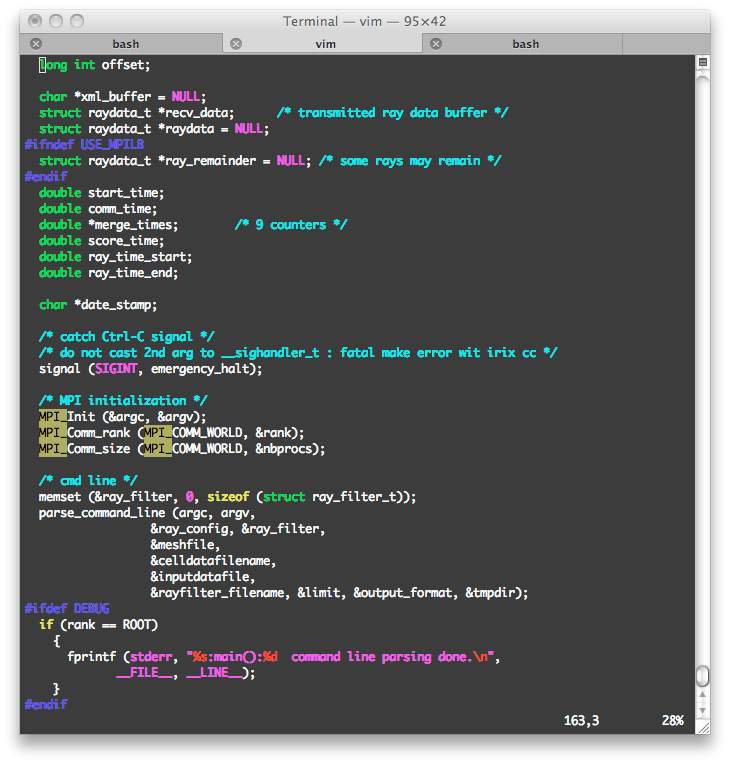
\includegraphics[height=12mm]{img/mpi-codelisting.png}};

        \node (nodeimagine) [
          shape             = cloud callout,
          cloud puffs       = 11,
          aspect            = 1.5,
          opacity           =.75,
          draw              = black!90!white, % colour of the border
          top color         = white,                % | filling of the node
          bottom color      = black!30!white, % |
          text              = black!90!white, % colour of the fonts
          thick,                              % thickness of the border
          above             = 5mm of nodehost,
          minimum height    = 25mm,
          minimum width     = 30mm,
          callout relative pointer={(285:5.5mm)},
        ]{};

        \node at (nodeimagine) {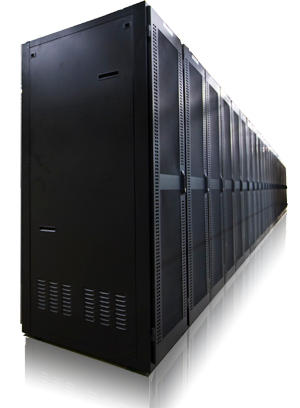
\includegraphics[width=15mm]{img/cluster.png}};
      \end{tikzpicture}
    \end{column}
    \begin{column}{.72\linewidth}
      \begin{block}{Research: {\color{black}Experimental methodologies}}
        \begin{itemize} 
        \item Assess distributed applications {\small(perfs, bugs)}
        \item SimGrid project: Simulator of distributed systems\\
          Correct modeling, efficient simulation
        \item Formal verification (model-checking)
        \end{itemize}
      \end{block}\vspace{-.5\baselineskip}

      \begin{block}{Teachings: {\color{black}Programming and Algorithms}}
        \begin{itemize}
        \item Introduction, Java/Scala, AlgoProg, C 2nd language
        \item System Prog; Ex-\{Algo dist, P2P, Distributed Prog\}
        \item PLM: Programmer's Learning Machine
        \end{itemize}
      \end{block}

      \structure{\large Outreach:} Unplugged Computer Science, etc.
    \end{column}
  \end{columns}
  \bigskip
  \begin{itemize}
    \item \structure{More info:}
      {\small\url{http://www.loria.fr/~quinson/} (\url{Martin.Quinson@loria.fr})}
    \end{itemize}
\end{frame}
%%%%%%%%%%%%%%%%%%%%%%%%%%%%%%%%%%%%%%%%%%%%%%%%%%%%%%%%%%%%%%%%%%%%%%%%%%%%%%%
\begin{frame}[squeeze]{About this module: \alert{Algorithmic and Programming}}
  \begin{block}{Programming? Let the computer do your work!}
    \begin{itemize}
    \item[] ~\vspace{-\baselineskip}
      \begin{itemize}
      \item How to explain what to do?
      \item How to make sure that it does what it is supposed to? That
        it is efficient?
      \item What if it does not?
      \end{itemize}
    \end{itemize}
  \end{block}
  \vspace{-.5\baselineskip}

  \begin{block}<2->{Module content and goals: }
    \begin{itemize}
    \item Introduction to Algorithmic
      \begin{itemize}
      \item Master theoretical basements (computer science is a science)
      \item Know some classical problem resolution techniques
      \item Know how to evaluate solutions (correctness, performance)
      \end{itemize}

    \item First steps in programming: learn-by-doing activity (you need to \textit{practice})
    \end{itemize}
  \end{block}
  \vspace{-.5\baselineskip}

  \begin{block}<3->{Other modules at Telecom Nancy}
    \begin{itemize}
    \item Prerequisites
      \begin{itemize}
      \item Tactical programming in Scala: \texttt{if}, \texttt{for}, methods
      \item Sense of logic, intuition (good math background helps)
      \end{itemize}
    \item Afterward: Object Oriented Programming; Object-Oriented Design

      \medskip
    \item[] {\small(please be patient, it's our first time with TOP before OOP)}
    \end{itemize}
  \end{block}
\end{frame}
%%%%%%%%%%%%%%%%%%%%%%%%%%%%%%%%%%%%%%%%%%%%%%%%%%%%%%%%%%%%%%%%%%%%%%%%%%
\begin{frame}{Module organization}
  \begin{block}{Time organization}
    \begin{itemize}
    \item 6 two-hours lectures {\small(CM, with Martin Quinson)}: 
      Concepts introduction
    \item 10 two-hours exercise session {\small(TD, with staff member%
      \footnote{ ~Olivier Festor, Mihai Andries, Juan Pablo Timpanaro, Martin Quinson.}%
      )}: Theoretical exercises
    \item 6 two-hours labs {\small(TP, with staff member$^1$)}: 
      Coding exercises
    \item Homework: Systematically finish the in-class exercises
    \end{itemize}
  \end{block}

  \begin{block}{Evaluation}
    \begin{itemize}
    \item Two hours table exam (closed book, only one sheet of notes allowed)
%    \item A project (to be given soon)
    \item Maybe some quiz at the beginning of labs
    \end{itemize}
  \end{block}
\end{frame}
%%%%%%%%%%%%%%%%%%%%%%%%%%%%%%%%%%%%%%%%%%%%%%%%%%%%%%%%%%%%%%%%%%%%%%%%%%%%%%

% %%%%%%%%%%%%%%%%%%%%%%%%%%%%%%%%%%%%%%%%%%%%%%%%%%%%%%%%%%%%%%%%%%%%%%%%%% 
% \begin{frame}{Module bibliography}
%   \begin{block}{Bibliography}
%     \begin{itemize}
%     \item \structure{Introduction to programming and object oriented design},
%       Nino \& Hosch.\\
%       Reference book. Very good for SE, less for CS (\$120).
%     \item \structure{Big Java}, Cay S. Horstman. Less focused on programming (\$110).
%     \item \structure{Programmer en java}, Claude Delannoy. \\
%       Bon livre de référence (au format poche -- 20\texteuro).
%     \item \structure{Entraînez-vous et maîtrisez Java par la pratique},
%       Alexandre Brillant. \\
%       Nombreux exercices corrigés (25\texteuro).
%     \end{itemize}
%   \end{block}

%   \begin{center}
%     \begin{tabular}{c c c c}
%       \includegraphics[width=2cm]{img/nino.jpg}&
%       \includegraphics[width=2cm]{img/horstmann.jpg}&
%       \includegraphics[width=14mm]{img/delannoy.jpg}&
%       \includegraphics[width=18mm]{img/brillant.jpeg}
%     \end{tabular}
%   \end{center}

%   \begin{block}{Webography}
%     \begin{itemize}
%     \item IUT Orsay (in french): \url{http://www.iut-orsay.fr/~balkansk/}
% %    \item Telecom Paris (in french): 
%     \end{itemize}
%   \end{block}
% \end{frame}
%%%%%%%%%%%%%%%%%%%%%%%%%%%%%%%%%%%%%%%%%%%%%%%%%%%%%%%%%%%%%%%%%%%%%%%%%%%%%%%
\begin{frame}{Syllabus}\label{Plan}
  \begin{enumerate}
  \item \structure{\hyperlink{intro}{Practical and Theoretical Foundations of Programming}}
    \begin{itemize}
    \item CS vs. SE; Abstraction for complex algorithms; Algorithmic efficiency.
    \end{itemize}

  \item \structure{\hyperlink{sort}{Iterative Sorting Algorithms}}
    \begin{itemize}
    \item Specification; Selection, Insertion and Bubble sorts.
    \end{itemize}

  \item \structure{\hyperlink{recurs}{Recursion}}
    \begin{itemize}
    \item Principles; Practice; Recursive sorts; Non-recursive From;
      Backtracking.
    \end{itemize}

  \item \structure{Dynamic Programming}
    \begin{itemize}
    \item Introduction; Greedy algorithms, Dynamic Programming.
    \end{itemize}

  \item \structure{Software Correction}
    \begin{itemize}
    \item Introduction; Specifying Systems; Hoare Logic; Proving Recursive
      Functions. 
    \end{itemize}

  % \item \structure{Testing Software}
  %   \begin{itemize}
  %   \item Testing techniques; Testing strategies; JUnit; Design By Contract.
  %   \end{itemize}

  \end{enumerate}

  \bigskip
  \centerline{This may change a bit to adapt and improve the class}
\end{frame}


% Figures pleine page : 122mm x 80mm



%%% Local Variables:
%%% coding: utf-8
\part{Practical and Theoretical Foundations of Programming}
\label{intro}\toc

%%%%%%%%%%%%%%%%%%%%%%%%%%%%%%%%%%%%%%%%%%%%%%%%%%%%%%%%%%%%%%%%%%%%%%%%%% 
\section{Introduction}
\subsection{From the problem to the code}
\begin{frame}[t]{Problems}
  \null\vspace{-.7\baselineskip}
  \centerline{\includegraphics[subfig=1,scale=.8]{fig/algo_problem_program.fig}}

  \medskip
  \concept{Provided by clients (or teachers ;)}

  \begin{block}{Problems}
    \begin{itemize}
    \item \structure{Problems are generic}
    \item[] Example: Determine the minimal value of a set of integers
    \end{itemize}
  \end{block}

  \begin{block}{Instances of a problem}
    \begin{itemize}
    \item \structure{The problem for a given data set}
    \item[] Example: Determine the minimal value of \{17, 6, 42, 24\}
    \end{itemize}    
  \end{block}
\end{frame}
%%%%%%%%%%%%%%%%%%%%%%%%%%%%%%%%%%%%%%%%%%%%%%%%%%%%%%%%%%%%%%%%%%%%%%%%%% 
\begin{frame}[t,squeeze]{Problems and Programs}
  \centerline{\includegraphics[subfig=2,scale=.8]{algo_problem_program.fig}}

  \begin{block}{Software systems {\color{black} (\textit{ie.}, Programs)}}
    \begin{itemize}
    \item Describes a set of actions to be achieved in a given order
    \item Doable (tractable) by computers
    \end{itemize}
  \end{block}\vspace{-.5\baselineskip}

  \begin{block}<2->{Problem Specification}
    \begin{itemize}
    \item Must be clear, precise, complete, without ambiguities
    \item[] Bad example: find position of minimal element
      {\small (two answers for \{4, 2, 5, 2, 42\})}
    \item[] Good example: Let $L$ be the set of positions for which the value is minimal.\\
      ~~~~~~~~~~~~~~~~~~~~Find the minimum of $L$
    \end{itemize}
  \end{block}\vspace{-.5\baselineskip}

  \begin{block}<2->{Using the Right Models}
    \begin{itemize}
    \item Need simple models to understand complex artifacts (ex: city
      map)
    \end{itemize}
  \end{block}
\end{frame}
%%%%%%%%%%%%%%%%%%%%%%%%%%%%%%%%%%%%%%%%%%%%%%%%%%%%%%%%%%%%%%%%%%%%%%%%%% 
\begin{frame}[t,squeeze]{Methodological Principles}
  \centerline{\includegraphics[subfig=3,scale=.8]{algo_problem_program.fig}}

  \begin{block}{Abstraction
      \color{black}{\normalsize think before coding (!)}}
    \begin{itemize}
    \item Describe how to solve the problem
    \end{itemize}
  \end{block}\vspace{-.8\baselineskip}

  \begin{block}{Divide, Conquer and Glue 
      \color{black}{\normalsize(top-down approach)}}
    \begin{itemize}
    \item \structure{Divide} complex problem into simpler sub-problems
      (think of Descartes)
    \item \structure{Conquer} each of them
    \item \structure{Glue} (combine) partial solutions into the big one
    \end{itemize}
  \end{block}\vspace{-.8\baselineskip}

  \begin{block}{Modularity}
    \begin{itemize}
    \item Large systems built of components: \textbf{modules}
    \item Interface between modules allow to mix and match them
    \end{itemize}
  \end{block}
\end{frame}
%%%%%%%%%%%%%%%%%%%%%%%%%%%%%%%%%%%%%%%%%%%%%%%%%%%%%%%%%%%%%%%%%%%%%%%%%% 
\begin{frame}[t]{Algorithms}
  \centerline{\includegraphics[subfig=4,scale=.8]{algo_problem_program.fig}}
  
  \begin{block}{Precise description {\color{black}of the}
      resolution process {\color{black}of a} well specified problem}
    \begin{itemize}
    \item Must be understandable (by human beings)
    \item Does not depend on target programming language, compiler or machine
    \item Can be an diagram (as pictured), but difficult for large problems
    \item Can be written in a simple language (called \textbf{pseudo-code})
    \end{itemize}
  \end{block}
  
  \begin{block}{``Formal'' definition}
    \begin{itemize}
    \item Sequence of actions acting on problem data to induce the expected result
    \end{itemize}
  \end{block}
\end{frame}
%%%%%%%%%%%%%%%%%%%%%%%%%%%%%%%%%%%%%%%%%%%%%%%%%%%%%%%%%%%%%%%%%%%%%%%%%% 
\newcommand{\fleche}[1]{$\underrightarrow{\text{\hbox to 5cm{\hfill#1\hfill}}}$}
\begin{frame}[t]{New to Algorithms?}
  \begin{block}{Not quite, you use them since a long time}\bigskip
    \begin{tabular}{p{31mm} c l}
      Lego bricks\texttrademark&\fleche{list of pictures}&Castle\\\\
      Ikea\texttrademark\ desk&\fleche{building instructions}&Desk\\\\
      Home location&\fleche{driving directions}&Party location\\\\
      Eggs, Wheal, Milk&\fleche{recipe}&Cake\\\\
      Two 6-digits integers&\fleche{arithmetic know-how}&sum 
    \end{tabular}
  \end{block}

  \begin{block}{And now}\bigskip
    \begin{tabular}{p{31mm} c l}
      List of students&\fleche{sorting algorithm}&Sorted list\\\\
      Maze map&\fleche{appropriated algorithm}&Way out\\\\

    \end{tabular}    
  \end{block}
\end{frame}
%%%%%%%%%%%%%%%%%%%%%%%%%%%%%%%%%%%%%%%%%%%%%%%%%%%%%%%%%%%%%%%%%%%%%%%%%% 
\subsection{Computer Science vs. Software Engineering}
\begin{frame}{Computer Science vs. Software Engineering}
  \begin{boitequote}{}
    \alert{Computer science} is a science of abstraction – creating the right
    model for a problem and devising the appropriate mechanizable
    technique to solve it.\hfill -- {\rm Aho and Ullman}
  \end{boitequote}\bigskip

  \begin{block}{NOT (only) Science of Computers}\medskip
    \begin{boitequote}{}
      Computer science is not more related to computers than\\
      Astronomy to telescopes.\hfill--~{\rm Dijkstra}
    \end{boitequote}
      
    \begin{itemize}
    \item Many concepts were framed and studied before the electronic computer
    \item To the logicians of the 20's, a \textit{computer} was a person with
      pencil and paper
    \end{itemize}
  \end{block}

  \begin{block}{Science of Computing}
    \begin{itemize}
    \item Automated problem solving
    \item Automated systems that produce solutions
    \item Methods to develop solution strategies for these systems
    \item Application areas for automatic problem solving
    \end{itemize}
  \end{block}
\end{frame}
%%%%%%%%%%%%%%%%%%%%%%%%%%%%%%%%%%%%%%%%%%%%%%%%%%%%%%%%%%%%%%%%%%%%%%%%%% 
\begin{frame}{Foundations of Computing}
  \begin{block}{Fundamental mathematical and logical structures}
    \begin{itemize}
    \item To understand computing
    \item To analyze and verify the correctness of software and hardware
    \end{itemize}
  \end{block}

  \begin{block}{Main issues of interest in Computer Science}
    \begin{itemize}
    \item \structure{Calculability}
      \begin{itemize}
      \item Given a problem, can we show whether there exist an
        algorithm solving it?
      \item Which are the problems for which no algorithm exist? How to
        categorize them?
      \end{itemize}
    \item \structure{Complexity}
      \begin{itemize}
      \item How long does my algorithm need to answer? (as function
        of input size)
      \item How much memory does it take?
      \item Is my algorithm optimal, or does a better one exist?
      \end{itemize}
    \item \structure{Correctness}
      \begin{itemize}
      \item Can we be certain that a given algorithm always reaches a solution?
      \item Can we be certain that a given algorithm always reaches
        the right solution?
      \end{itemize}
    \end{itemize}
  \end{block}
\end{frame}
%%%%%%%%%%%%%%%%%%%%%%%%%%%%%%%%%%%%%%%%%%%%%%%%%%%%%%%%%%%%%%%%%%%%%%%%%% 
\begin{frame}{Software Engineering vs. Computer Science}
  \concept{Producing technical answers to consumers' needs}

  \begin{block}{Software Engineering Definition}
    \begin{itemize}
    \item Study of methods for producing and evaluating software
    \end{itemize}
  \end{block}
  
  \begin{block}<2->{Life cycle of a software
      {\color{black}\normalsize (\textit{much} more details to come later)}}\medskip
    \centerline{\includegraphics{fig/algo_cycleV.fig}}
    \begin{itemize}
    \item \structure{Global design:} Identify application modules
    \item \structure{Detailed design:} Specify within modules
    \end{itemize}
  \end{block}
\end{frame}
%%%%%%%%%%%%%%%%%%%%%%%%%%%%%%%%%%%%%%%%%%%%%%%%%%%%%%%%%%%%%%%%%%%%%%%%%% 
\begin{frame}{As future IT engineers, you need both CS and SE}
  \begin{block}{Without Software Engineering}
    \begin{itemize}
    \item Your production will not match consumers' expectation
    \item You will induce more bugs and problems than solutions
    \item Each program will be a pain to develop and to maintain for you
    \item You won't be able to work in teams
    \end{itemize}
  \end{block}

  \begin{block}{Without Computer Science}
    \begin{itemize}
    \item Your programs will run slowly, deal only with limited data sizes
    \item You won't be able to tackle difficult (and thus well paid) issues
    \item You won't be able to evaluate the difficulty of a task (and
      thus its price)
    \item You will reinvent the wheel (badly)
    \end{itemize}
  \end{block}

  \begin{block}<2->{Two approaches of the same issues}
    \begin{itemize}
    \item \structure{Correctness:}
      CS $\leadsto$ prove algorithms right; 
      SE $\leadsto$ chase (visible) bugs
    \item \structure{Efficiency:} CS $\leadsto$ theoretical bounds on
      performance, optimality proof;\\
      \hspace{16.6mm}SE $\leadsto$ optimize execution time and
      memory usage

    \end{itemize}
  \end{block}
\end{frame}
%%%%%%%%%%%%%%%%%%%%%%%%%%%%%%%%%%%%%%%%%%%%%%%%%%%%%%%%%%%%%%%%%%%%%%%%%% 
\section{Designing Algorithms for Complex Problems}\sectionpage
\begin{frame}{There are always several ways to solve a problem}
  \begin{block}<+->{Choice criteria between algorithms}
    \begin{itemize}
    \item \structure{Correctness:} provides the right answer
    \item \structure{\alert<+>{Simplicity:}}
      KISS! (jargon acronym for \textit{keep it simple, silly})
    \item \structure{Efficiency:} fast, use little memory
    \item \structure{Stability:} small change in input does not change output
    \end{itemize}
  \end{block}\vspace{-.5\baselineskip}

  \begin{block}<.->{Real problems ain't easy}
    \begin{itemize}
    \item They are not fixed, but \alert{dynamic}
      \begin{itemize}
      \item Specification helps users understanding the problem better\\
        That is why they often add wanted functionalities after specification
      \item My text editor is v23.2.1 
        {\small(hundreds of versions for ``just a text editor'')}
      \end{itemize}

    \item They are \alert{complex} (composed of several interacting entities)
    \end{itemize}
  \end{block}

  \visible<.->{
    \begin{boitequote}{\small"Epigrams in Programming", by Alan J. Perlis.}
      In computing, turning the obvious into the useful is a living definition
      of the word "frustration".
    \end{boitequote}
  }
\end{frame}
%%%%%%%%%%%%%%%%%%%%%%%%%%%%%%%%%%%%%%%%%%%%%%%%%%%%%%%%%%%%%%%%%%%%%%%%%% 
\begin{frame}{Dealing with Complexity}
  \begin{block}{Some classical design principles help}
    \begin{itemize}\vspace{-.2\baselineskip}
    \item \structure{Composition}: split problem in simpler
      sub-problems and compose pieces
    \item \structure{Abstraction}: forget about details and focus on
      important aspects
    \end{itemize}    
  \end{block}\vspace{-.5\baselineskip}

  \begin{block}{Object Oriented Programming}
    \begin{itemize}\vspace{-.2\baselineskip}
    \item Classical answer to specification complexity and dynamicity
      Encapsulation, polymorphism, heritage, \ldots
    % \item \structure{Encapsulation:} Divide complexity into manageable units
    % \item \structure{Polymorphism:} Use one (specialized) block instead of the
    %   expected one
    % \item \structure{Heritage:} Allow to factorize behavior between related
    %   units
    \item That's one way to \structure{design applications} in a modular manner
    \item Other approaches exists, but none have the same momentum currently
    \end{itemize}
  \end{block}\vspace{-.5\baselineskip}

  \visible<2>{
    \begin{block}{Rest of this module}
      \begin{itemize}%\vspace{-.2\baselineskip}
      \item How to write each block / units / objects to be composed in OOP
      \end{itemize}
    \end{block}\vspace{-.7\baselineskip}
    
    \begin{block}{Why algorithms before OOP and not the contrary?}
      \begin{itemize}\vspace{-.2\baselineskip}
      \item Coding at small before programming at large
      \item (that's an endless debate, pros and cons for both approaches)
%      \item Every mainstream languages (including Java) are object oriented
%      \item Research in CS education shows that ``object first'' is a better
%        approach
      \end{itemize}
    \end{block}
  }
\end{frame}

%%%%%%%%%%%%%%%%%%%%%%%%%%%%%%%%%%%%%%%%%%%%%%%%%%%%%%%%%%%%%%%%%%%%%%%%%% 
\subsection{Composition}
\begin{frame}{Dealing with complexity: Composition}
  \begin{block}{Composite structure}
    \begin{itemize}
    \item \structure{Definition:} a software system composed of
      manageable pieces
    \item[\Smiley] The smaller the component, the easier it is to
      build and understand
    \item[\Frownie] The more parts, the more possible interactions
      there are between parts
    \item[$\Rightarrow$] the more complex the resulting structure
    \item Need to balance between simplicity and interaction minimization
    \end{itemize}
  \end{block}

  \begin{block}<2->{Good example: audio system}\medskip
    Easy to manage because:
    \begin{itemize}
    \item each component has a carefully specified function
    \item components are easily integrated
    \item i.e. the speakers are easily connected to the amplifier
    \end{itemize}
  \end{block}
\end{frame}

%%%%%%%%%%%%%%%%%%%%%%%%%%%%%%%%%%%%%%%%%%%%%%%%%%%%%%%%%%%%%%%%%%%%%%%%%% 
\begin{frame}[squeeze]{Composition counter-example (1/2)}
  \begin{block}{Rube Goldberg machines}
    \begin{itemize}
    \item Device not obvious, modification unthinkable
    \item Parts lack intrinsic relationship to the solved problem
    \item Utterly high complexity
    \end{itemize}
  \end{block} \vspace{-\baselineskip}

  \begin{columns}
    \begin{column}{.6\linewidth}
      \begin{block}{Example: Tax collection machine}\bigskip
        \includegraphics[width=\linewidth]{fig/algo_rube-localtaxes.fig}
      \end{block}
    \end{column}
    \begin{column}{.4\linewidth}
      \begin{enumerate}
      \item[A.] Taxpayer sits on cushion
      \item[B.] Forcing air through tube
      \item[C.] Blowing balloon
      \item[D.] Into candle
      \item[E.] Explosion scares dog
      \item[F.] Which pull leash
      \item[G.] Dropping ball
      \item[H.] On teeter totter
      \item[I.] Launch plans
      \item[J.] Which tilts lever
      \item[K.] Then Pitcher
      \item[L.] Pours water on plant
      \item[M.] Which grows, pulling chain
      \item[N.] Hand lifts the wallet
      \end{enumerate}    
    \end{column}
  \end{columns}
\end{frame}
%%%%%%%%%%%%%%%%%%%%%%%%%%%%%%%%%%%%%%%%%%%%%%%%%%%%%%%%%%%%%%%%%%%%%%%%%% 
\begin{frame}[squeeze]{Composition counter-example (2/2)}
  \begin{block}{Rube Goldberg's toothpaste dispenser}\smallskip
    \centerline{\includegraphics[width=.7\linewidth]{fig/algo_rube-toothpaste.fig}}
  \end{block}

  Such over engineered solutions should obviously remain jokes
\end{frame}
%%%%%%%%%%%%%%%%%%%%%%%%%%%%%%%%%%%%%%%%%%%%%%%%%%%%%%%%%%%%%%%%%%%%%%%%%% 
\subsection{Abstraction}
\begin{frame}{Dealing with complexity: Abstraction}
  \begin{block}{Abstraction}
    \begin{itemize}
    \item Dealing with components and interactions without worrying
      about details
    \item Not ``vague'' or ``imprecise'', but focused on few relevant properties
    \item Elimination of the irrelevant and amplification of the
      essential
    \item Capturing commonality between different things
    \end{itemize}
  \end{block}

  \begin{columns}
    \begin{column}{.3\linewidth}
      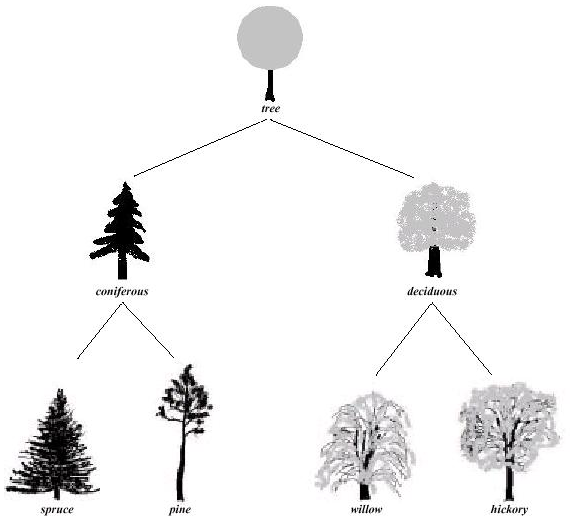
\includegraphics[width=\linewidth]{fig/algo_abstracting_trees.png}      
    \end{column}

    \begin{column}{.7\linewidth}
      \begin{block}<2->{Abstraction in programming}
        \begin{itemize}
        \item Think about what your components should do before
        \item Ie, abstract their \textbf{interface} before coding
        \visible<2->{
        \centerline{\includegraphics[scale=.8]{fig/algo_contract.fig}}~~~~~~~~~}
        \item Show your interface, hide your implementation
        \end{itemize}
      \end{block}
    \end{column}
  \end{columns}
  
\end{frame}
%%%%%%%%%%%%%%%%%%%%%%%%%%%%%%%%%%%%%%%%%%%%%%%%%%%%%%%%%%%%%%%%%%%%%%%%%% 
\section{Crash Course on Scala}\sectionpage
\begin{frame}{Scala? Why??}

  \begin{block}{Main reason for me: simplicity}
    \begin{itemize}
    \item Most of you are absolute beginners to programming
    \item I want to talk about algorithms, not to bother you about syntax
    \end{itemize}
  \end{block}

  \begin{block}{Scala has much more to offer}
    \begin{itemize}
    \item OOP (mixin+singleton), functional, properties, type inference, JVM-based \ldots
    \item<2-> But we don't care for now: \alert{see it as a simple language}
    \item<2-> You'll learn its true beauty later on
    \end{itemize}
  \end{block}
\end{frame}
%%%%%%%%%%%%%%%%%%%%%%%%%%%%%%%%%%%%%%%%%%%%%%%%%%%%%%%%%%%%%%%%%%%%%%%%%
\begin{frame}[fragile]{Starting Scala}
  
  \structure{\large Installation:} Get it from \url{http://scala-lang.org/} (version 2.10 at least)
  \smallskip

  \begin{block}{Executing your code}
    \begin{columns}
      \begin{column}{.28\linewidth}
        \begin{boitecode}{myfile.scala}
println("Hello, friends")

        \end{boitecode}
      \end{column}
      \begin{column}{.22\linewidth}
        \begin{boiteshell}{Run directly}
\$ scala myfile.scala          
Hello, friends
\$
        \end{boiteshell}
      \end{column}
      \begin{column}{.38\linewidth}
        \begin{boiteshell}{Compile first}
\$ scalac -Xscript toto myfile.scala          
\$ scala toto
Hello, friends
\$      \end{boiteshell}
      \end{column}
    \end{columns}
    %%%
    \begin{columns}
      \begin{column}{.3\linewidth}
        \begin{boitecode}{myscript}
#!/usr/bin/scala
!#
println("Hello, friends")
        \end{boitecode}
        \begin{boiteshell}{Turn it into a script}
\$ chmod +x myscript
\$ ./myscript
Hello, friends
\$      \end{boiteshell}
      \end{column}
      \begin{column}{.4\linewidth}
        \begin{boiteshell}{Run interactively}
\$ scala
Welcome to Scala [...]

scala> \structure{println("Hello, friends")}
Hello, friends

scala> \structure{:load myfile.scala}
Loading toto.scala...
Hello, friends
        \end{boiteshell}
      \end{column}

    \end{columns}
  \end{block}
\end{frame}
%%%%%%%%%%%%%%%%%%%%%%%%%%%%%%%%%%%%%%%%%%%%%%%%%%%%%%%%%%%%%%%%%%%%%%%%%%%%
\begin{frame}{Getting Started in Scala}
  \structure{\large Declaring a variable:} {\large\framebox{\texttt{var x:Int = 0}} }
  \smallskip

  \begin{tabular}{c@{~$\leadsto$~}l}
    \texttt{var} & because that's a \textbf{var}iable\\
    \texttt{x}   & name of that variable (its label)\\
    \texttt{:Int}& type of this variable (what it can store)\\
    \texttt{= 0}  & initial value (mandatory)
  \end{tabular}

  \begin{itemize}
  \item You can often omit the type (it's inferred): \framebox{\texttt{var x = 0}}
  \end{itemize}

  \begin{block}{Some Scala data types}
    \begin{itemize}
    \item \structure{Int:} for integer values,  \structure{Double:} for dot numbers
    \item \structure{Boolean:} \texttt{true/false}, \structure{String:} \texttt{"some chars together"}
    \end{itemize}
  \end{block}

  \begin{block}<2->{Declaring a value}
    \begin{itemize}
    \item If your "variable" is constant, make it a value:
      ~\framebox{\texttt{\alert{val} answer:Int = 42}}
      \smallskip
      
    \item Seen as good style in Scala \hfill%
      \textit{\small mutable stateful objects are the new spaghetti code}
    \item Allows to detect errors, may produce faster code, easy multithreading.
    \item Do values unless you must use variables
    \end{itemize}
  \end{block}

\end{frame}
%%%%%%%%%%%%%%%%%%%%%%%%%%%%%%%%%%%%%%%%%%%%%%%%%%%%%%%%%%%%%%%%%%%%%%%%%%%%
\begin{frame}[fragile]{The Scala Syntax}
  \begin{block}{Looping}\smallskip
  \begin{columns}
    \begin{column}{.3\linewidth}
      \begin{Verbatim}[gobble=8,fontsize=\small,frame=single,commandchars=+[\]]
        +textrm[+textbf[while]] (+textit[condition]) {
          +textit[instructions]
        }
      \end{Verbatim}
    \end{column}

    \begin{column}{.3\linewidth}
      \begin{Verbatim}[gobble=8,fontsize=\small,frame=single,commandchars=+[\]]
        +textrm[+textbf[do]] {
          +textit[instructions]
        } +textrm[+textbf[while]] (+textit[condition])
      \end{Verbatim}
    \end{column}

    \begin{column}{.37\linewidth}
      \begin{Verbatim}[gobble=8,fontsize=\small,frame=single,commandchars=+[\]]
        +textrm[+textbf[for]] (+textit[i] +textrm[+textbf[+recvVal]] 0 +textrm[+textbf[to]] 10 +textrm[+textbf[by] 2]) {
          // i in 0,2,4,6,8,10
        }
      \end{Verbatim}
    \end{column}
  \end{columns}
  \end{block}

  \bigskip
  \begin{block}{Methods and functions}\smallskip
    \begin{columns}
      \begin{column}{.37\linewidth}
        \begin{Verbatim}[gobble=9,fontsize=\small,frame=single,commandchars=+[\]]
         +textrm[+textbf[def]] +textit[sayIt](msg:String) {
           print(msg)
         }
        \end{Verbatim}
      \end{column}

      \begin{column}{.55\linewidth}
        \begin{Verbatim}[gobble=9,fontsize=\small,frame=single,commandchars=+[\]]
         +textrm[+textbf[def]] +textit[max3](x:Int, y:Int, z:Int)+alert[:Int =] {
           val m = if (x>y) x else y
           if (m>z) {
             return m
           } else {
             return z
           }
         }
        \end{Verbatim}
      \end{column}
    \end{columns}
  \end{block}
\end{frame}
%%%%%%%%%%%%%%%%%%%%%%%%%%%%%%%%%%%%%%%%%%%%%%%%%%%%%%%%%%%%%%%%%%%%%%%%%%%%%%
\begin{frame}[fragile]{Pattern matching: cascading if / else if are over}
  
  \begin{columns}
    \begin{column}{.57\linewidth}
      \begin{Verbatim}[gobble=8,fontsize=\footnotesize,frame=single,commandchars=+[\]]
        +textit[name] +textrm[+textbf[match]] {
          +textrm[+textbf[case]] +textit["Martin"] => +textit[println("Hey there")]
          +textrm[+textbf[case]] +textit["Gerald"] => +textit[println("Hello")]
          +textrm[+textbf[case]] _ +hspace[10.7mm]=> +textit[println("Gnii?")]
        }
      \end{Verbatim}
    \end{column}
    \begin{column}{.42\linewidth}
      \begin{itemize}
      \item Veeery powerful construct
      \item Any expression can be filtered
      \item The default case is mandatory
      \end{itemize}
    \end{column}
  \end{columns}

  \begin{columns}
    \begin{column}{.73\linewidth}
      \begin{Verbatim}[gobble=8,fontsize=\footnotesize,frame=single,commandchars=+[\]]
        +textit[name] +textrm[+textbf[match]] {
          +textrm[+textbf[case]] +textit["Martin"] | +textit["Gerald"] => +textit[println("Hey there")]
          +textrm[+textbf[case]] _ +hspace[27.7mm]=> +textit[println("Gniii?")]
        }
      \end{Verbatim}      
    \end{column}
    \begin{column}{.265\linewidth}
      ~
    \end{column}
  \end{columns}

 \begin{columns}
    \begin{column}{.73\linewidth}
      \begin{Verbatim}[gobble=8,fontsize=\footnotesize,frame=single,commandchars=+[\]]
        +textit[age] +textrm[+textbf[match]] {
          +textrm[+textbf[case]] i +textrm[+textbf[if]] i<20 => println("Hey dude!")
          +textrm[+textbf[case]] i +textrm[+textbf[if]] i<30 => println("Hello young man")
          +textrm[+textbf[case]] _ +hspace[11.4mm]=> println("Hello Sir")
        }
      \end{Verbatim}      
    \end{column}
    \begin{column}{.265\linewidth}
      ~
    \end{column}
  \end{columns}

 \begin{columns}
    \begin{column}{.73\linewidth}
      \begin{Verbatim}[gobble=8,fontsize=\footnotesize,frame=single,commandchars=+[\]]
        +textit[(x,y)] +textrm[+textbf[match]] {
          +textrm[+textbf[case]] (0,0) => println("Origin")
          +textrm[+textbf[case]] (_,0) => println("Abscissa")
          +textrm[+textbf[case]] (0,_) => println("Ordinate")
          +textrm[+textbf[case]] (_,_) => println("Random")
        }
      \end{Verbatim}      
    \end{column}
    \begin{column}{.265\linewidth}
      ~
    \end{column}
  \end{columns}
\end{frame}
%%%%%%%%%%%%%%%%%%%%%%%%%%%%%ù
\begin{frame}

  \Concept{There is much more to Scala}
  \medskip

  \centerline{But that's all you need to know for now\ldots}
\end{frame}

\section{Comparing Algorithms' Efficiency}\sectionpage
\begin{frame}{Comparing Algorithms' Efficiency}
  \concept{There are always more than one way to solve a problem}
  \begin{block}<+->{Choice criteria between algorithms}
    \begin{itemize}
    \item \structure{Correctness:} provides the right answer
    \item \structure{Simplicity:} \textit{not} Rube Goldberg's machines 
    \item \alert{Efficiency:} fast, use little memory
    \item \structure{Stability:} small change in input does not change output
    \end{itemize}
  \end{block}\vspace{-.5\baselineskip}

  \begin{block}<+->{Empirical efficiency measurements}
    \begin{itemize}
    \item Code the algorithm, benchmark it and use runtime statistics
    \item[\Frownie] Several factors impact performance: \\
      {\small machine, language, programmer, compiler, compiler's options,
      operating system, \ldots}
    \item[$\Rightarrow$] Performance not generic enough for comparison
    \end{itemize}
  \end{block}\vspace{-.5\baselineskip}

  \begin{block}<+->{Mathematical efficiency estimation}
    \begin{itemize}
    \item Count amount of basic instruction as function of input size
    \item[\Smiley] Simpler, more generic and often sufficient
    \item[] {\small(true in theory;
      in practice, optimization necessary \textbf{in addition} to this)}
    \end{itemize}
  \end{block}
\end{frame}
%%%%%%%%%%%%%%%%%%%%%%%%%%%%%%%%%%%%%%%%%%%%%%%%%%%%%%%%%%%%%%%%%%%%%%%%%% 
\subsection{Best case, worst case, average analysis}
\begin{frame}[fragile,squeeze]{Best case, worst case, average analysis}
  \concept{Algorithm running time depends on the data}
  \begin{block}<+->{Example: Linear search in an array}\vspace{-.5\baselineskip}
    \begin{center}      
    \begin{minipage}{.7\linewidth}
    \begin{Verbatim}[frame=single,fontsize=\footnotesize,gobble=6]
      def linearSearch(val:Int, tab:Array[Int]): Boolean = {
        for (i <- 0 to tab.length-1) 
          if (tab(i) == val)
            return true;
        return false
      }
    \end{Verbatim}      
    \end{minipage}
    \end{center}\vspace{-.8\baselineskip}
    \begin{itemize}
    \item Case 1: search whether 42 is in \{42, 3, 2, 6, 7, 8, 12, 16, 17, 32, 55, 44, 12\}\\
      answer found after one step
    \item Case 2: search whether 4 is in \{42, 3, 2, 6, 7, 8, 12, 16, 17, 32, 55, 44, 12\}\\
      need to traverse the whole array to decide (n steps)
    \end{itemize}
  \end{block}\vspace{-.5\baselineskip}

  \begin{block}<+->{Counting the instructions to run in each case}
    \begin{itemize}
    \item $t_{min}$: \#instructions for the best case inputs 
    \item $t_{max}$: \#instructions for the worst case inputs 
    \item $t_{avg}$: \#instructions  on average 
      {\small(average of values coefficiented by probability)}\\
      $t_{avg}=p_1t_1+p_2t_2+\ldots+p_nt_n$
    \end{itemize}
  \end{block}
\end{frame}
%%%%%%%%%%%%%%%%%%%%%%%%%%%%%%%%%%%%%%%%%%%%%%%%%%%%%%%%%%%%%%%%%%%%%%%%%% 
\begin{frame}[fragile]{Linear search runtime analysis}
  \begin{center}\vspace{-.6\baselineskip}      
    \begin{minipage}{.6\linewidth}
    \begin{Verbatim}[frame=single,fontsize=\footnotesize,gobble=6]
        for (i <- 0 to tab.length-1)
          if (tab(i) == val)
            return true
        return false
    \end{Verbatim}      
    \end{minipage}
    \end{center}\vspace{-.3\baselineskip}

    \begin{itemize}
    \item For simplicity, let's assume the value is in the array,
      positions are equally likely
    \item Let's count tests (noted \alert{t}), 
      additions (noted \alert{a}) and 
      value changes (noted \alert{c})
    \end{itemize}


  \begin{block}{Best case: searched data in first position}
    \begin{itemize}
    \item 1 value change (i=0); 2 tests  (loop boundary + equality)
    \item $ t_{min}=\alert{c}+2\alert{t}$
    \end{itemize}
  \end{block}\vspace{-.5\baselineskip}
  \begin{block}{Worst case: searched data in last position}
    \begin{itemize}
    \item 1 value change (i=0); \{2 tests, 1 change, 1 addition (i+=1)\} per loop
    \item $t_{max}=c+n\times(2t+1c+1a)=(n+1)\times\alert{c}+2n\times\alert{t}+n\times\alert{a}$
    \end{itemize}
  \end{block}\vspace{-.5\baselineskip}

  \begin{block}<2->{Average case: searched data in position $p$ with
      probability $\frac{1}{n}$}
    \begin{itemize}
    \item {\small$\displaystyle t_{avg}
        =c+\sum_{p\in[1,n]}\frac{1}{n}\times (2t+c+a)\times p
        \uncover<3->{=c+\frac{1}{n}\times(2t+c+a)\times\sum_{p\in[1,n]}p}$}\\
      {\small$\uncover<4->{\displaystyle t_{avg}
        =c+\frac{n(n-1)}{2n}\times(2t+c+a)}
        \uncover<5->{
        =(n-1)\times\alert{t}+\frac{n+1}{2}\times\alert{c}+\frac{n-1}{2}\times\alert{a}}
        $}
    \end{itemize}
  \end{block}
\end{frame}
%%%%%%%%%%%%%%%%%%%%%%%%%%%%%%%%%%%%%%%%%%%%%%%%%%%%%%%%%%%%%%%%%%%%%%%%%% 
\begin{frame}{Simplifying equations}
  \concept{\fbox{$t_{avg}=(n-1)\times t+\frac{n+1}{2}\times
      c+\frac{n-1}{2}\times a$} is too complicated}

  \begin{block}<2->{Reducing amount of variables}
    \begin{itemize}
    \item To simplify, we only count the most expensive operations
    \item But which it is is not always clear...
    \item Let's take write accesses \alert{c} (classical but arbitrary choice)
    \end{itemize}
  \end{block}

  \begin{block}<3->{Focusing on dominant elements}
    \begin{itemize}
    \item We can forget about constant parts if there is n operations
    \item We can forget about linear parts if there is $n^2$ operations
    \item \ldots
    \item Only consider the most dominant elements when
      $n$ is very big
    \item[$\Rightarrow$] This is called \textbf{\alert{asymptotic complexity}}
    \end{itemize}
  \end{block}
\end{frame}
%%%%%%%%%%%%%%%%%%%%%%%%%%%%%%%%%%%%%%%%%%%%%%%%%%%%%%%%%%%%%%%%%%%%%%%%%% 
\subsection{Asymptotic complexity}
\begin{frame}{Asymptotic Complexity: Big-O notation}
  \begin{block}{Mathematical definition}
    \begin{itemize}
    \item Let $T(n)$ be a non-negative function
    \item \fbox{$T(n) \in O(f(n))$} 
      $\Leftrightarrow \exists \text{ constants } c, n_0 
      \text{ so that } \forall n>n_0,$ \fbox{$T(n)\le c\times f(n)$}
    \item f(n) is an upper bound of T(n) \ldots
    \item[\ldots] after some point, and with a constant multiplier
    \end{itemize}
  \end{block}

  \begin{block}{Application to runtime evaluation}
    \begin{itemize}
    \item $T(n)\in O(n^2)\Rightarrow$ when n is big enough, you need less than $n^2$ steps
    \item This gives a upper bound
    \end{itemize}
  \end{block}
\end{frame}
%%%%%%%%%%%%%%%%%%%%%%%%%%%%%%%%%%%%%%%%%%%%%%%%%%%%%%%%%%%%%%%%%%%%%%%%%% 
\begin{frame}[fragile]{Big-O examples}
  \begin{block}{Example 1: Simplifying a formula}
    \begin{itemize}
    \item Linear search: $t_{avg}=(n-1)\times t+\frac{n+1}{2}\times
      c+\frac{n-1}{2}\times a$ $\Rightarrow$ \framebox{$T(n)=O(n)$}
    \item Imaginary example: $T(n)=17n^2+\frac{32}{17}n+\pi$
      $\Rightarrow$ \framebox{$T(n)=O(n^2)$}
    \item If T(n) is constant, we write T(n)=O(1)
    \end{itemize}
  \end{block}

  \begin{block}{Practical usage}
    \begin{itemize}
    \item Since this is a upper bound, $T(n)=O(n^3)$ is also true when $T(n)=O(n^2)$
    \item But not as relevant
    \end{itemize}
  \end{block}

  \begin{block}<2->{Example 2: Computing big-O values directly}\medskip
    \begin{center}
      \begin{minipage}{.5\linewidth}        
      \begin{Verbatim}[label=array initialization,gobble=8,frame=single]
        for (i <- 0 to tab.length-1) 
          tab(i) = 0
      \end{Verbatim}
      \end{minipage}
    \end{center}
    \vspace{-\baselineskip}
    \begin{itemize}
    \item We have $n$ steps, each of them doing a constant amount of work
    \item $T(n) = c\times n$ ~~ $\Rightarrow$ ~~ $T(n) = O(n)$
    \item[] (don't bother counting the constant elements)
    \end{itemize}
  \end{block}
\end{frame}
%%%%%%%%%%%%%%%%%%%%%%%%%%%%%%%%%%%%%%%%%%%%%%%%%%%%%%%%%%%%%%%%%%%%%%%%%% 
\begin{frame}{Big-Omega notation}
  \begin{block}{Mathematical definition}
    \begin{itemize}
    \item Let $T(n)$ be a non-negative function
    \item \fbox{$T(n) \in \Omega(f(n))$} 
      $\Leftrightarrow \exists \text{ constants } c, n_0 
      \text{ so that } \forall n>n_0,$ \fbox{$T(n)\ge c\times f(n)$}
    \item Similar to Big-O, but gives a \alert{lower} bound
    \item Note: similarly to before, we are interested in big lower bounds
    \end{itemize}
  \end{block}

  \begin{block}{Example: $T(n)=c_1\times n^2+c_2\times n$}
    \begin{itemize}
    \item $T(n)=c_1\times n^2+c_2\times n\ge c_1\times n^2$ ~~~ $\forall n>1$\\
      $T(n)\ge c\times n^2$ for $c>c_1$
    \item Thus, $T(n)=\Omega(n^2)$
    \end{itemize}
  \end{block}
\end{frame}
%%%%%%%%%%%%%%%%%%%%%%%%%%%%%%%%%%%%%%%%%%%%%%%%%%%%%%%%%%%%%%%%%%%%%%%%%% 
\begin{frame}{Theta notation}
  \begin{block}{Mathematical definition}
    \begin{itemize}
    \item $T(n)\in\Theta(g(n))$ if and only if 
      $T(n)\in O(g(n))$ and $T(n)\in\Omega(g(n))$
    \end{itemize}
  \end{block}

  \centerline{\includegraphics[scale=1.3]{fig/algo_theta.fig}}

  \begin{block}{Example}\vspace{-\baselineskip}
    \begin{center}      
      \resizebox{.7\linewidth}{!}{\begin{tabular}{l|c|c|c|c|c}\cline{2-5}
      \multicolumn{1}{l}{}&
      \multicolumn{1}{|l|}{}&
      n=10&n=1000&n=100000\\\cline{2-5}

      \multirow{2}*{$\Theta(n)$}&n&10&1000&$10^5$&\multirow{2}*{seconds}\\
      &100n&1000&$10^5$&$10^7$\\
      \cline{2-5}

      \multirow{2}*{$\Theta(n^2)$}&$n^2$&100&$10^6$&$10^{10}$
      &\multirow{2}*{minutes}\\
      &$100n^2$&$10^4$&$10^8$&$10^{12}$\\
      \cline{2-5}

      \multirow{2}*{$\Theta(n^3)$}&$n^3$&1000&$10^9$&$10^{15}$
      &\multirow{2}*{hours}\\
      &$100n^2$&$10^5$&$10^{11}$&$10^{17}$\\
      \cline{2-5}

      \multirow{2}*{$\Theta(2^n)$}&$2^n$&1024&$>10^{301}$&$\infty$
      &\multirow{2}*{\ldots}\\
      &$100\times 2^n$&$>10^5$&$10^{305}$&$\infty$\\
      \cline{2-5}

      \multirow{2}*{$\log(n)$}&$\log(n)$&3.3&$9.9$&$16.6$&\\
      &$100\log(n)$&$332.2$&$996.5$&$1661$\\
      \cline{2-5}
    \end{tabular}}
    \end{center}
  \end{block}
\end{frame}
%%%%%%%%%%%%%%%%%%%%%%%%%%%%%%%%%%%%%%%%%%%%%%%%%%%%%%%%%%%%%%%%%%%%%%%%%% 
\begin{frame}{Classical mistakes}
  \begin{block}<+->{Mistake notations}
    \begin{itemize}
    \item Indeed, we have  $O(\log(n))=O(n)=O(n^2)=O(n^3)=O(2^n)$ \\
      \visible<+->{{\small Because it's an upper bound; to be correct we should
          write $\subset$ instead of =}}
    \item Likewise, we have
      $\Omega(\log(n))=\Omega(n)=\Omega(n^2)=\Omega(n^3)=\Omega(2^n)$\\
      \visible<.->{{\small Because it's a lower bound; we should write
          $\supset$ instead of =}}
    \item We only have  $\Theta(\log(n))\neq\Theta(n)\neq\Theta(n^2)
      \neq\Theta(n^3)\neq\Theta(2^n)$\vspace{.3\baselineskip}
    \visible<+->{
    \item[] (but in practice, everybody use O() as if it were $\Theta()$ --
      although that's wrong)}
    \end{itemize}
  \end{block}

  \begin{block}<+->{Mistake worst case and upper bounds}
    \begin{itemize}
    \item Worst case is the input data leading to the longest operation time
    \item Upper bound gives indications on increase rate when input size
      increases 
    \item[] (same distinction between best case and lower bound)
    \end{itemize}
  \end{block}
\end{frame}
%%%%%%%%%%%%%%%%%%%%%%%%%%%%%%%%%%%%%%%%%%%%%%%%%%%%%%%%%%%%%%%%%%%%%%%%%% 
\begin{frame}{Asymptotic Complexity in Practice}
  \begin{block}{Rules to compute the complexity of an algorithm}
    \begin{description}
    \item[Rule 1:] Complexity of a sequence of instruction: Sum of
      complexity of each
    \item[Rule 2:] Complexity of basic instructions (test, read/write
      memory): O(1)
    \item[Rule 3:] Complexity of \texttt{if}/\texttt{switch}
      branching: Max of complexities of branches
    \item[Rule 4:] Complexity of loops: Complexity of content $\times$
      amount of loop
    \item[Rule 5:] Complexity of methods: Complexity of content
    \end{description}
  \end{block}\vspace{-.5\baselineskip}

  \begin{block}<2->{Simplification rules}\vspace{-.3\baselineskip}
    \begin{itemize}
    \item \structure{Ignoring the constant}:
    \item[] If f(n) = O({\small $k\times g(n)$}) 
            and $k>0$ is constant
            then f(n) = O(\small{g(n)})
    \item \structure{Transitivity}
    \item[] If f(n) = O({\small g(n)}) 
            and g(n) = O({\small h(n)}) 
            then f(n) = O(\small{h(n)})
    \item \structure{Adding big-Os}
    \item[] If A(n) = O({\small f(n)}) 
            and B(n) = O({\small g(n)}) 
            then A(n)+B(n) = O(\small{max({\footnotesize f(n), g(n)})})\\
            \hspace{77.7mm}= O({\small f(n)+g(n)})\vspace{-.7\baselineskip}
    \item \structure{Multiplying big-Os}
    \item[] If A(n) = O({\small f(n)}) 
            and B(n) = O({\small h(n)}) 
            then $A(n)\times B(n)$ = O({\small $f(n)\times g(n)$})
    \end{itemize}
  \end{block}
\end{frame}
%%%%%%%%%%%%%%%%%%%%%%%%%%%%%%%%%%%%%%%%%%%%%%%%%%%%%%%%%%%%%%%%%%%%%%%%%% 
\begin{frame}[fragile]{Some examples}
  \begin{block}{Example 1: {\color{black}\normalsize
      \fbox{\texttt{a=b;}} $\Rightarrow \Theta(1)$ (constant time)}}
  \end{block}\vspace{-\baselineskip}

  \begin{block}{Example 2}\vspace{-\baselineskip}
    \begin{columns}
      \begin{column}{.1\linewidth}~\end{column}
      \begin{column}{.3\linewidth}
        \begin{Verbatim}[gobble=8]
        var sum=0;
        for (i <- 1 to n)
          sum += n;
      \end{Verbatim}
      \end{column}
      \begin{column}{.3\linewidth}
        $\Theta(n)$
      \end{column}
    \end{columns}
  \end{block}

  \begin{block}{Example 3}\vspace{-\baselineskip}
    \begin{columns}
      \begin{column}{.1\linewidth}~\end{column}
      \begin{column}{.3\linewidth}
        \begin{Verbatim}[gobble=8]
        var sum=0;
        for (i <- 1 to n)
          for (j <- 1 to n)
            sum += 1
        for (k <- 0 to n-1)
          A(k) = k;
      \end{Verbatim}
      \end{column}
      \begin{column}{.3\linewidth}
        $\Theta(1)+\Theta(n^2)+\Theta(n)=\Theta(n^2)$
      \end{column}
    \end{columns}
  \end{block}

  \begin{block}{Example 4}\vspace{-\baselineskip}
    \begin{columns}
      \begin{column}{.1\linewidth}~\end{column}
      \begin{column}{.3\linewidth}
        \begin{Verbatim}[gobble=8]
        var sum=0;
        for (i <- 1 to n)
          for (j <- 1 to i)
            sum += 1
      \end{Verbatim}
      \end{column}
      \begin{column}{.3\linewidth}
        $\Theta(1)+O(n^2)=O(n^2)$
        one can also show $\Theta(n^2)$
      \end{column}
    \end{columns}
  \end{block}

  \begin{block}{Example 5}\vspace{-\baselineskip}
    \begin{columns}
      \begin{column}{.1\linewidth}~\end{column}
      \begin{column}{.3\linewidth}
        \begin{Verbatim}[gobble=8]
        var sum=0; var i=0
        while (i<n) {
          sum +=1
          i = i * 2
        }
      \end{Verbatim}
      \end{column}
      \begin{column}{.3\linewidth}
        $\Theta(\log(n))$
        $\log$ is due to the $i\times2$
      \end{column}
    \end{columns}
  \end{block}
\end{frame}
%%%%%%%%%%%%%%%%%%%%%%%%%%%%%%%%%%%%%%%%%%%%%%%%%%%%%%%%%%%%%%%%%%%%%%%%%% 
\begin{frame}{Going further on Algorithm Complexity}
  \vspace{-.5\baselineskip}
  \begin{block}<+->{Problems' Classification}
    \begin{itemize}\vspace{-.2\baselineskip}
    \item Problems can also be sorted in class of complexities (not only
      algorithms)\\
      {\small depending on the best existing algorithm to solve them}
    \item Showing that no better algorithm exist for a given problem:
      \alert{Calculability}
    \item Multi-million question: \alert{P=NP?}
      \begin{description}
      \item[P:] polynomial algorithm to find the solution exists
      \item[NP:] {\small candidate solution eval. in polynomial time, but no
          known polynomial algo}
      \item[NP-complete:] set of NP problems for which if one P algorithm is
        found, \\
        it's applicable to every other NP-complete problems
      \end{description}
    \end{itemize}
  \end{block}\vspace{-.5\baselineskip}

  \begin{block}<+->{\alert{Time} is not the only metric of interest:
      \alert{Space} too}
    \begin{itemize}\vspace{-.2\baselineskip}
    \item In computation, there is a sort of tradeoff between space and time\\
      {\small  Faster algorithms need to pre-compute elements \ldots
        requiring more storage memory}
    \end{itemize}
  \end{block}\vspace{-.5\baselineskip}

  \begin{block}<+->{So does \alert{Energy} nowadays!}
    \begin{itemize}\vspace{-.2\baselineskip}
    \item Computational power of CPU grows linearly with frequency;\\
      Energy consumption grows (more than) quadratically with frequency
    \item To save energy (and money), split your task on several
      slower cores \\
      {\small Parallel algorithms are the way to go (but it's \textit{ways}
        harder)}
    \end{itemize}
  \end{block}
\end{frame}
%%%%%%%%%%%%%%%%%%%%%%%%%%%%%%%%%%%%%%%%%%%%%%%%%%%%%%%%%%%%%%%%%%%%%%%%%% 
\section{Algorithmic Stability}\sectionpage
\begin{frame}[fragile]{Algorithmic stability}

  \begin{block}{Computers use fixed precision numbers}
    \begin{itemize}
    \item<+-> 10+1=11
    \item<+-> $10^{10}+1=10000000001$
    \item<+-> $10^{16}+1=10000000000000001$
    \item<+-> $10^{17}+1=10000000000000000\alert{0}=10^{17}$
    \end{itemize}
  \end{block}

  \begin{block}<+->{What is the value of $\sqrt{2^2}$?}
    \begin{itemize}
    \item Old computers though it was 1.9999999
    \end{itemize}
  \end{block}

  \begin{block}<.->{Other example}
    \begin{columns}
      \begin{column}{.27\linewidth}
        \begin{Verbatim}[gobble=9]
          while (value < 2E9) 
            value += 1E-8;
        \end{Verbatim}
      \end{column}
      \begin{column}{.6\linewidth}
        This is an infinite loop\\
        {\small(because when $value=10^9$, $value+10^{-8}=value$)}
      \end{column}
    \end{columns}
  \end{block}

  \medskip
  \uncover<+->{
  \concept{Numerical instabilities are to be killed to predict weather,}

  \concept{simulate a car crash or control a nuclear power plant}}

  \medskip\uncover<+->{(but this is all \textit{ways} beyond our goal this year ;)}
\end{frame}
%%%%%%%%%%%%%%%%%%%%%%%%%%%%%%%%%%%%%%%%%%%%%%%%%%%%%%%%%%%%%%%%%%%%%%%%%% 
\section{Conclusion}
\begin{frame}[squeeze]{Conclusion of this chapter}
  ~\vspace{-1.5\baselineskip}
  \begin{block}<+->{What tech guys tend to do when submitted a problem}
    \vspace{-.4\baselineskip}
    \begin{itemize}
    \item They code it directly, and rewrite everything once they
      understood
    \item And rewrite everything to improve performance
    \item And rewrite everything when the code needs to evolve
    \end{itemize}
  \end{block}\vspace{-.6\baselineskip}

  \begin{block}<+->{What managers tend to do when submitted a problem}
    \vspace{-.4\baselineskip}
    \begin{itemize}
    \item They write up a long and verbose specification
    \item They struggle with the compiler in vain
    \item Then they pay a tech guy 
      {\small(and pay too much since they don't get the grasp)}
    \end{itemize}
  \end{block}\vspace{-.6\baselineskip}

  \begin{block}<+->{What theoreticians tend to do when submitted a problem}
    \vspace{-.4\baselineskip}
    \begin{itemize}
    \item They write a terse but formal specification
    \item They write an algorithm, and prove its optimality
    \item[] (the algorithm never gets coded)
    \end{itemize}
  \end{block}\vspace{-.6\baselineskip}

  \begin{block}<+->{What good programmers do when submitted a problem}
    \vspace{-.4\baselineskip}
    \begin{itemize}
    \item They write a clear specification
    \item They come up with a clean design
    \item They devise efficient data structures and algorithms
    \item Then (and only then), they write a clean and efficient code
    \item They ensure that the program does what it is supposed to do
    \end{itemize}
  \end{block}
\end{frame}
%%%%%%%%%%%%%%%%%%%%%%%%%%%%%%%%%%%%%%%%%%%%%%%%%%%%%%%%%%%%%%%%%%%%%%%%%% 
\begin{frame}[squeeze]{Choice criteria between algorithms}
  \begin{block}{Correctness}
    \begin{itemize}
    \item \structure{Provides the right answer}
    \item This crucial issue is delayed a bit further
    \end{itemize}
  \end{block}\vspace{-.6\baselineskip}
  \begin{block}{Simplicity}
    \begin{itemize}
    \item \structure{Keep it simple, silly}
    \item Simple programs can evolve (problems and client's wishes often do)
    \item Rube Goldberg's machines cannot evolve
    \end{itemize}
  \end{block}\vspace{-.6\baselineskip}
  \begin{block}{Efficiency}
    \begin{itemize}
    \item \structure{Run fast, use little memory, dissipate little energy}
    \item Asymptotic complexity must remain polynomial
    \item Note that you cannot have a decent complexity with the wrong
      data structure
    \item You still want to test the actual performance of your code in practice
    \end{itemize}
  \end{block}\vspace{-.6\baselineskip}
  \begin{block}{Numerical stability}
    \begin{itemize}
    \item \structure{Small change in input does not change output}
    \item Advanced issue, critical for numerical simulations (but beyond our
      scope)
    \end{itemize}
  \end{block}
\end{frame}\part{Iterative Sorting Algorithms}
\label{sort}\toc
%%%%%%%%%%%%%%%%%%%%%%%%%%%%%%%%%%%%%%%%%%%%%%%%%%%%%%%%%%%%%%%%%%%%%%%%%% 
\section{Problem Specification}
%%%%%%%%%%%%%%%%%%%%%%%%%%%%%%%%%%%%%%%%%%%%%%%%%%%%%%%%%%%%%%%%%%%%%%%%%% 
\begin{frame}[squeeze]{Sorting Problem Specification}
  \begin{block}{Input data}
    \begin{itemize}
    \item A sequence of N comparable items $<a_1,a_2,a_3,\ldots,a_N>$
    \item Items are \textit{comparable} iff $\forall a, b$ in set,
      either \underline{$a<b$} or \underline{$a>b$} or \underline{$a=b$}
    \end{itemize}
  \end{block}\vspace{-.7\baselineskip}

  \begin{block}{Result}
    \begin{itemize}
    \item Permutation\footnote{reordering} $<a_1',a_2',a_3',\ldots,a_N'>$ so
      that: $a_1'\leq a_2'\leq a_3'\leq\ldots\leq a_N'$
    \end{itemize}
  \end{block}\vspace{-.7\baselineskip}

  \begin{block}{Sorting complex items}
    \begin{itemize}
    \item For example, if items represent students, they encompass name, class,
      grade
    \item \structure{Key:} value used for the sort 
    \item \structure{Extra data:} other data associated to items, permuted
      along with the keys
    \end{itemize}
  \end{block}\vspace{-.7\baselineskip}

  \begin{block}{Problem simplification}
    \begin{itemize}
    \item We assume that items are chars or integers to be sorted in
      ascending order\\ (no loss of generality)
    \end{itemize}
  \end{block}\vspace{-.7\baselineskip}

  \begin{block}{Memory consideration}
    \begin{itemize}
    \item Sort \textit{in place}, without any auxiliary array.
      Memory complexity: O(1)
    \end{itemize}
  \end{block}
\end{frame}
%%%%%%%%%%%%%%%%%%%%%%%%%%%%%%%%%%%%%%%%%%%%%%%%%%%%%%%%%%%%%%%%%%%%%%%%%% 
\section{Selection Sort}
\subsection{Presentation}
\begin{frame}{Selection Sort}
  \begin{block}{Big lines}
    \begin{itemize}
    \item First get the smallest value, and put it in first position
    \item Then get the second smallest value, and put it in second position
    \item and so on for all values
    \end{itemize}
  \end{block}

  \begin{columns}
    \begin{column}{.4\linewidth}
      \begin{block}{Example:}\bigskip
        \includegraphics<1| handout:0>[subfig=1]{fig/sort_selection.fig}
        \includegraphics<2| handout:0>[subfig=2]{fig/sort_selection.fig}
        \includegraphics<3| handout:0>[subfig=3]{fig/sort_selection.fig}
        \includegraphics<4| handout:0>[subfig=4]{fig/sort_selection.fig}
        \includegraphics<5| handout:0>[subfig=5]{fig/sort_selection.fig}
        \includegraphics<6| handout:0>[subfig=6]{fig/sort_selection.fig}
        \includegraphics<7| handout:0>[subfig=7]{fig/sort_selection.fig}
        \includegraphics<8| handout:0>[subfig=8]{fig/sort_selection.fig}
        \includegraphics<9| handout:0>[subfig=9]{fig/sort_selection.fig}
        \includegraphics<10-| handout:1>[subfig=10]{fig/sort_selection.fig}
      \end{block}
    \end{column}

    \begin{column}{.55\linewidth}
      \visible<11->{
        \begin{boitecode}{\only<11>{Pseudo}\only<12->{Scala} code}
          \structure{\visible<12->{/*} for each element, do: \visible<12->{*/}}

          \visible<12->{for (i <- 0 to length-1) \{}

          ~

          ~~\structure{\visible<12->{/*} (1) search min on [i;N] \visible<12->{*/}}

          \visible<13->{
            ~~var minpos=i
            
            ~~for (j <- i to length-1) \{ \structure{/* $\forall j\in[i;length-1]$ */}

            ~~~~if (tab(j) < tab(minpos)) \{

            ~~~~~~minpos = j

            ~~~~\}

            ~~\}
          }
          
          ~

          ~~\structure{\visible<12->{/*} (2) put min first \visible<12->{*/}}

          \visible<14->{
            ~~temp=tab(i)

            ~~tab(i)=tab(minpos)

            ~~tab(minpos)=temp

          }
          \visible<12->{\}}

          ~
        \end{boitecode}
      }
    \end{column}
  \end{columns}
\end{frame}
%%%%%%%%%%%%%%%%%%%%%%%%%%%%%%%%%%%%%%%%%%%%%%%%%%%%%%%%%%%%%%%%%%%%%%%%%% 
\subsection{Discussion}
\begin{frame}[fragile]{Selection sort discussion}
  \begin{block}{We apply a very generic approach here:}
    \begin{itemize}
    \item Do right now what you can, delay the rest for later (put min first)
    \item Progressively converge to what you are looking for (sort the remaining)
    \end{itemize}
  \end{block}

  \begin{columns}
    \begin{column}{.37\linewidth}
        \begin{boitecode}{}
for (i <- 0 to length-1) \{
  var minpos=i
  for (j <- i to length-1) \{
    if (tab(j) < tab(minpos)) \{
      minpos = j
    \}
  \}
  temp=tab(i)
  tab(i)=tab(minpos)
  tab(minpos)=temp
\}
        \end{boitecode}
    \end{column}

    \begin{column}{.6\linewidth}
      \begin{block}<2->{Memory Analysis}
        \begin{itemize}
        \item 2 extra variables\\
          {\small(only one at the same time, actually)}
        \item[$\Rightarrow$] Constant amount of extra memory
        \item[$\Rightarrow$] Space complexity is $O(1)$
        \item $O(1)$ is the smallest complexity $\leadsto$ $\Theta(1)$
        \end{itemize}
      \end{block}      
    \end{column}
  \end{columns}
  
  \begin{block}<3->{Time Analysis}
    \begin{itemize}
    \item Forget about constant times, focus on loops!
    \item<4-> Two interleaved loops which length is \textit{at most} N
    \item<5->[$\Rightarrow$] Time complexity is $O(N^2)$
    \end{itemize}
  \end{block}
\end{frame}
%%%%%%%%%%%%%%%%%%%%%%%%%%%%%%%%%%%%%%%%%%%%%%%%%%%%%%%%%%%%%%%%%%%%%%%%%% 
\begin{frame}[fragile]{Finer analysis of selection sort's time performance}
  \begin{columns}
    \begin{column}{.37\linewidth}
        \begin{boitecode}{}
for (i <- 0 to length-1) \{
  var minpos=i
  for (j <- i to length-1)
    if (tab(j) < tab(minpos))
      minpos = j
  temp=tab(i)
  tab(i)=tab(minpos)
  tab(minpos)=temp
\}
        \end{boitecode}
    \end{column}

    \begin{column}{.6\linewidth} 
      \begin{block}<+->{Best case, worst case, average case}
        \begin{itemize}
        \item No matter the order of the data,\\
          'selection sort' does the same
        \item[$\Rightarrow$] $t_{min}=t_{max}=t_{avg}$
        \end{itemize}
      \end{block}     
    \end{column}
  \end{columns}\vspace{-\baselineskip}

  \begin{block}<+->{Counting steps more precisely (but only dominant term)}
    \begin{itemize}\vspace{-.2\baselineskip}
    \item $\displaystyle T(N)=\sum_{i\in[1,N]}\left(\sum_{j\in{[i,N[}}1\right)$
      \visible<+->{$=\displaystyle\sum_{i\in[1,N]}(N-i)$
      $=\displaystyle\sum_{i\in[1,N]}N-\sum_{i\in[1,N]}i$\\\smallskip
      \hspace{9.5mm}$= N^2-\frac{N\times(N+1)}{2}$
      $= N^2-\frac{N^2+N}{2}$
      $=\frac{1}{2}N^2-\frac{1}{2}N$
      $=\frac{1}{2}(N^2-N)$}

    \item<+-> \structure{Let's prove that $T(n)\in\Omega(n^2)$.}
      For that, we want:
    \item<.-> $\exists c, n_0 / \forall N>n_0,$ 
      \framebox{$\frac{1}{2}(N^2-N)\ge cN^2$} 
      \visible<+->{
        $\!\Leftarrow\!$ \framebox{$N^2-N\ge 2cN^2$}
        $\!\Leftarrow\!$ \framebox{$N-1\ge 2cN$}
      }
    \item<+-> So, we want $\exists c, n_0 / \forall N>n_0, N\ge \frac{1}{1-2c}$
    \item<+-> Let's take anything for c ($\neq\frac{1}{2}$), and
      $n_0=\frac{1}{1-2c}$. Trivially gives what we want.
      
      % \smallskip
    \item<.->[] \centerline{\alert{$T(n)\in\Theta(n^2)$}}

    \end{itemize}
  \end{block}
\end{frame}
%%%%%%%%%%%%%%%%%%%%%%%%%%%%%%%%%%%%%%%%%%%%%%%%%%%%%%%%%%%%%%%%%%%%%%%%%%   
\section{Insertion Sort}
\subsection{Presentation}
\begin{frame}[squeeze]{Insertion Sort}
  \begin{columns}
    \begin{column}{.8\linewidth}
      \begin{block}<+->{How do you sort your card deck?}
        \begin{itemize}
        \item No human would apply \textit{selection sort} to sort a deck!
        \end{itemize}
      \end{block}\vspace{-.7\baselineskip}
      \begin{block}<.->{Algorithm used most of the time to sort a card deck:}
        \begin{itemize}
        \item[1.] If the cards \#1 and \#2 need to be swapped, do it
        \item[2.] Insert card \#3 at its position in the [1,2] part of the deck
        \item[3.] Insert card \#4 at its position in the [1,3] part of the deck
        \item[] \ldots
        \end{itemize}
      \end{block}\vspace{-.7\baselineskip}
    \end{column}

    \begin{column}{.2\linewidth}
      \includegraphics<+->[width=\linewidth]{fig/sort_insertion_cards.fig}
    \end{column}
  \end{columns}\vspace{-.4\baselineskip}


  \begin{columns}
    \begin{column}{.68\linewidth}
      \begin{block}<.->{Finding the common pattern}
        \begin{itemize}
        \item Step n ($\ge2$) is ``insert card \#(n+1) into [1,n]''
        \item<+-> Step 1 =  insert the 2. card into [1,1]
        \item<.-> We may add a Step 0 to generalize the pattern{\small\\
            (that's a no-op)}
        \end{itemize}
      \end{block}\vspace{-\baselineskip}

      \begin{alertblock}<12->{Algorithm big lines}%\medskip
      \framebox{\begin{minipage}{1.0\linewidth}\begin{tabbing}
            For each element\\
            ~~\=Find insertion position\\
            \>Move element to position
      \end{tabbing}\vspace{-1\baselineskip}\end{minipage}}
      \end{alertblock}
    \end{column}

    \begin{column}{.3\linewidth}
      \begin{block}<4->{This is \textit{Insertion Sort}}\medskip
        \includegraphics<-.| handout:0>[subfig=1]{fig/sort_insertion.fig}
        \includegraphics<+| handout:0>[subfig=2]{fig/sort_insertion.fig}
        \includegraphics<+| handout:0>[subfig=3]{fig/sort_insertion.fig}
        \includegraphics<+| handout:0>[subfig=4]{fig/sort_insertion.fig}
        \includegraphics<+| handout:0>[subfig=5]{fig/sort_insertion.fig}
        \includegraphics<+| handout:0>[subfig=6]{fig/sort_insertion.fig}
        \includegraphics<+| handout:0>[subfig=7]{fig/sort_insertion.fig}
        \includegraphics<+| handout:0>[subfig=8]{fig/sort_insertion.fig}
        \includegraphics<+| handout:0>[subfig=9]{fig/sort_insertion.fig}
        \includegraphics<+-| handout:1>[subfig=10]{fig/sort_insertion.fig}
      \end{block}      
    \end{column}
  \end{columns}
\end{frame}
%%%%%%%%%%%%%%%%%%%%%%%%%%%%%%%%%%%%%%%%%%%%%%%%%%%%%%%%%%%%%%%%%%%%%%%%%% 
\begin{frame}{Writing the \textit{insertion sort} algorithm}
  \vspace{-.5\baselineskip}
  \begin{block}{Fleshing the big lines}\smallskip
  \begin{columns}
    \begin{column}{.3\linewidth}
      \framebox{\begin{minipage}{1.0\linewidth}\small\begin{tabbing}
            For each element\\
            ~~\=Find insertion point\\
            \>Move element to position
      \end{tabbing}\vspace{-1\baselineskip}\end{minipage}}      
    \end{column}

    \begin{column}{.7\linewidth}
      \begin{itemize}\vspace{-.8\baselineskip}
      \item Finding the insertion point is easy (searching loop)
      \item Moving to position is a bit harder: ``make room''
      \item We have to \textit{shift} elements one after the other
      \end{itemize}
    \end{column}
  \end{columns}
  \end{block}

  \only<+| handout:0>{\centerline{\includegraphics[subfig=1]{fig/sort_insertion_shift.fig}}}
  \only<+| handout:0>{\centerline{\includegraphics[subfig=2]{fig/sort_insertion_shift.fig}}}
  \only<+| handout:0>{\centerline{\includegraphics[subfig=3]{fig/sort_insertion_shift.fig}}}
  \only<+| handout:0>{\centerline{\includegraphics[subfig=4]{fig/sort_insertion_shift.fig}}}
  \only<+-|
  handout:1>{\centerline{\includegraphics[subfig=5]{fig/sort_insertion_shift.fig}}}  

  \vspace{-1.5\baselineskip}
  \uncover<+->{
  \begin{itemize}
  \item Shifting elements induce a loop also
  \item We can do both searching insertion point and shifting at the same time
  \end{itemize}}

  \uncover<+->{
    \begin{columns}
      \begin{column}{.9\linewidth}
    \begin{boitecode}{}
      \visible<+->{for (i $<$- \alert{1} to length-1) \{ \structure{/* i: boundary between unsorted/sorted areas*/}}

      ~~\structure{/* save current value (it this case, that's O) */}

       \visible<+->{~~val tmp = tab(i)}

       ~~\structure{/* shift to right any element on the left being smaller than tmp */}

       \visible<+->{
         ~~var j = i

         ~~while (j$>$0 \&\& tab(j-1)$>$tmp) \{ \structure{/* while previous cell exists and is bigger */}

         ~~~~tab(j) = tab(j-1) \structure{/* copy that element */}

         ~~~~j = j -1 \structure{/* consider the next element */}

         ~~\}}

       ~~\structure{/* put tmp in cleared position */}

       \visible<+->{~~tab(j)=tmp}

       \}

    \end{boitecode}        
      \end{column}
    \end{columns}
  }
\end{frame}
%%%%%%%%%%%%%%%%%%%%%%%%%%%%%%%%%%%%%%%%%%%%%%%%%%%%%%%%%%%%%%%%%%%%%%%%%% 
\section{Bubble Sort}
\subsection{Presentation}
\begin{frame}{Bubble Sort}
  \begin{itemize}
  \item All these sort algorithms are quite difficult to write. Can we do simpler?
  \item<+-> Like ``while it's not sorted, sort it a bit''
  \end{itemize}

  \begin{columns}
    \begin{column}{.5\linewidth}
      \begin{block}<+->{Detecting that it's sorted}\medskip
        \framebox{\begin{minipage}{1.0\linewidth}\scriptsize\begin{tabbing}
          for (i $<$- 0 to length-2)\\
          ~~~\structure{/* if these two values are badly sorted */}\\
          ~~~if (tab(i)$>$tab(i+1))\\
          ~~~~~~return false\\
          return true
      \end{tabbing}\vspace{-1\baselineskip}\end{minipage}}
      \end{block}
    \end{column}

    \begin{column}{.5\linewidth}
      \begin{block}<+->{How to ``sort a bit?''}
        \begin{itemize}
        \item We may just swap these two values
        \end{itemize}
        \centerline{\framebox{\begin{minipage}{1.0\linewidth}\scriptsize\begin{tabbing}
          val tmp=tab(i)\\
          tab(i)=tab(i+1)\\
          tab(i+1)=tmp
        \end{tabbing}\vspace{-1\baselineskip}\end{minipage}}}
      \end{block}
    \end{column}
  \end{columns}
  \bigskip

  \begin{columns}
    \begin{column}{.4\linewidth}
      \begin{block}<+->{All together}
        \begin{itemize}
        \item Add boolean variable to check whether it sorted
        \end{itemize}
      \end{block}
    \end{column}
    \begin{column}{.6\linewidth}
      \visible<.->{
        \centerline{\framebox{\begin{minipage}{1.0\linewidth}\scriptsize\begin{tabbing}
          var swapped = true\\
          while (swapped) \{ \structure{/* until we do one traversal without swap */}\\
          ~~~swapped = false\\
          ~~~for (i $<$- 0 to length-2)\\
          ~~~~~~if (tab(i) $>$ tab(i+1)) \{ \structure{/* if these 2 values are badly sorted */}\\
          ~~~~~~~~~\structure{/* swap them */}\\
          ~~~~~~~~~val tmp = tab(i)\\
          ~~~~~~~~~tab(i) = tab(i+1)\\
          ~~~~~~~~~tab(i+1) = tmp\\
          ~~~~~~~~~\structure{/* and remember we swapped something */}\\
          ~~~~~~~~~swapped = true\\
          ~~~~~~\}\\
          \} \structure{/* repeat until a traversal without swapping */}
        \end{tabbing}\vspace{-1\baselineskip}\end{minipage}}}}
    \end{column}
  \end{columns}
\end{frame}
%%%%%%%%%%%%%%%%%%%%%%%%%%%%%%%%%%%%%%%%%%%%%%%%%%%%%%%%%%%%%%%%%%%%%%%%%% 
\section{Conclusion}
\begin{frame}{Conclusion on Iterative Sorting Algorithms}
  \begin{block}{Cost Theoretical Analysis}\medskip

    \begin{tabular}{|l|c|c|c|}\hline
      \structure{Amount of comparisons}&\structure{Best Case}&
      \structure{Average Case}&\structure{Worst Case}\\\hline

      Selection Sort&$O(n^2)$&$O(n^2)$&$O(n^2)$\\\hline
      Insertion Sort&$O(n)$&$O(n^2)$&$O(n^2)$\\\hline
      Bubble Sort&$O(n)$&$O(n^2)$&$O(n^2)$\\\hline 

%      \hline
%      Quick Sort&$O(n\log(n))$&$O(n\log(n))$&$O(n^2)$\\\hline
%      Merge Sort&$O(n\log(n))$&$O(n\log(n))$&$O(n\log(n))$\\\hline      
    \end{tabular}
  \end{block}

  \begin{block}{Which is the best in practice?}
    \begin{itemize}
    \item We will explore practical performance during the lab
    \item But in practice, bubble sort is \alert{awfully slow} and should never be used
    \end{itemize}    
  \end{block}

  \begin{block}<2->{Is it optimal?}
    \begin{itemize}
    \item The lower bound is $\Omega(n\log(n))$ -- cf. TD lab
    \item Some other algorithms achieve it (Quick Sort, Merge Sort)
    \item We come back on these next week
    \end{itemize}    
  \end{block}

  \begin{flushright}
    (this ends the first lecture)    
  \end{flushright}
\end{frame}

\part{Recursion}
\label{recurs}\mypartpage
\begin{Coupe}
\section{Introduction}
%%%%%%%%%%%%%%%%%%%%%%%%%%%%%%%%%%%%%%%%%%%%%%%%%%%%%%%%%%%%%%%%%%%%%%%%%%%%%% 
\begin{frame}{Divide \& Conquer}
  \vspace{-.5\baselineskip}
  \begin{block}{Classical Algorithmic Pattern}
    \begin{itemize}
    \item When the problem is too complex to be solved directly, decompose it
    \end{itemize}
  \end{block}

  \begin{block}{When/How is it applicable?}
    \begin{enumerate}
    \item \structure{Divide:} Decompose problem into (simpler/smaller)
      sub-problems
    \item \structure{Conquer:} Solve sub-problems
    \item \structure{Glue:} Combine solutions of sub-problems
      to a solution as a whole
    \end{enumerate}
  \end{block}\medskip

  \vspace{-6.5\baselineskip}~\hfill{\includegraphics[scale=.8]{fig/rec_divide_conquer.fig}}~~~~~

  \smallskip
  \begin{boitequote}{Martin Luther King}%
    You don't have to see the whole staircase, just take the first step.
  \end{boitequote}
  
\end{frame}

%%%%%%%%%%%%%%%%%%%%%%%%%%%%%%%%%%%%%%%%%%%%%%%%%%%%%%%%%%%%%%%%%%%%%%%%%%%%%% 
\begin{frame}{Recursion}
  \visible<+->{\concept{Divide \& Conquer + sub-problems similar to big one}}
  \medskip

  \begin{block}<+->{Recursive object}
    \begin{itemize}
    \item \alert{Defined using itself}
    \item<+-> \structure{Examples}:
      \begin{itemize}
      \item $\alert{U}(n)=3\times \alert{U}(n-1)+1$ ; 
        \only<-3>{$\alert{U}(0)=1$}%
        \only<4| handout:0>{\underline{$\alert{U}(0)=1$}}
      \item Char \alert{string} = either a char followed by a \alert{string},
        or  \only<-3>{empty string}\only<4| handout:0>{\underline{empty
            string}} 
      \end{itemize}
    \item<.-> Often possible to rewrite the object, in a non-recursive way
      {\small(said \textit{iterative way})}
      \medskip
    \end{itemize}
  \end{block}

  \begin{block}<+->{Base case(s)}
    \begin{itemize}
    \item Trivial cases that can be solved directly
    \item Avoids infinite loop
    \end{itemize}
  \end{block}
\end{frame}
%%%%%%%%%%%%%%%%%%%%%%%%%%%%%%%%%%%%%%%%%%%%%%%%%%%%%%%%%%%%%%%%%%%%%%%%%%%%%% 
\begin{frame}{When the base case is missing\ldots}
  \begin{columns}
    \begin{column}{.55\linewidth}
      \begin{block}<2->{There's a Hole in the Bucket {\small(traditional)}}
        {\footnotesize%There's a hole in the bucket, dear Liza, dear Liza,\\
          There's a hole in the bucket, dear Liza, a \alert{hole}.
          
          % So fix it dear Henry, dear Henry, dear Henry,\\
          So fix it dear Henry, dear Henry, fix it.
          
          % With what should I fix it, dear Liza, dear Liza,\\
          With what should I fix it, dear Liza, with what?

          % With straw, dear Henry, dear Henry, dear Henry,\\
          With straw, dear Henry, dear Henry, with \alert{straw}.

          % But the straw is too long, dear Liza, dear Liza,\\
          The straw is too long, dear Liza, too long.
          
          % So cut it dear Henry, dear Henry, dear Henry,\\
          So cut it dear Henry, dear Henry, cut it!
          
          % With what should I cut it, dear Liza, dear Liza,\\
          With what should I cut it, dear Liza, with what?
          
          % Use the hatchet, dear Henry, dear Henry, dear Henry,\\
          Use the hatchet, dear Henry, the \alert{hatchet}.
          
          % But the hatchet's too dull, dear Liza, dear Liza,\\
          The hatchet's too dull, dear Liza, too dull.

          % So, sharpen it, dear Henry, dear Henry, dear Henry,\\
          So sharpen it dear Henry, dear Henry, sharpen it!

          % With what should I sharpen it, dear Liza, dear Liza,\\
          With what should I sharpen, dear Liza, with what?

          % Use the stone, dear Henry, dear Henry, dear Henry,\\
          Use the stone, dear Henry, dear Henry, the \alert{stone}.

          % But the stone is too dry, dear Liza, dear Liza,\\
          The stone is too dry, dear Liza, too dry.

          % So wet it, dear Henry, dear Henry, dear Henry,\\
          So wet it dear Henry, dear Henry, wet it.
          
          % With what should I wet it, dear Liza, dear Liza,\\
          With what should I wet it, dear Liza, with what?
          
          % With water, dear Henry, dear Henry, dear Henry,\\
          With water, dear Henry, dear Henry, \alert{water}.
          
          % With what should I carry it, dear Liza, dear Liza,\\
          With what should I carry it dear Liza, with what?
          
          % Use the bucket dear Henry, dear Henry, dear Henry,\\
          Use the bucket, dear Henry, dear Henry, the \alert{bucket}!
          
          % There's a hole in the bucket, dear Liza, dear Liza,\\
          There's a hole in the bucket, dear Liza, a \alert{hole}.}
      \end{block}      
    \end{column}\hspace{-2em}
    \begin{column}{.5\linewidth}
      ~\vspace{2\baselineskip}
      \begin{block}{Classical Aphorism}
        ~~~To understand \alert{recursion},\\
        ~~~you first have to understand \alert{recursion}
      \end{block}

      \begin{block}<3->{Recursive Acronyms}
        \begin{itemize}
        \item \alert{G}NU is \alert{N}ot \alert{U}nix
        \item \alert{P}HP: \alert{H}ypertext \alert{P}reprocessor
        \item \alert{P}NG's \alert{N}ot \alert{G}IF
        \item \alert{W}ine \alert{I}s \alert{N}ot an \alert{E}mulator
        \item {\small\alert{V}isa \alert{I}nternational \alert{S}ervice
            \alert{A}ssociation}
        \item {\small\underline{\alert{H}\textsc{ird}} of
            \alert{U}nix-\alert{R}eplacing \alert{D}aemons\\
            \alert{H}urd of \alert{I}nterfaces \alert{R}epresenting
            \alert{D}epth}
        \item \alert{Y}our \alert{O}wn \alert{P}ersonal \alert{Y}OPY
        \end{itemize}
      \end{block}
    \end{column}
  \end{columns}

  \bigskip This is naturally to be avoided in algorithms
\end{frame}
%%%%%%%%%%%%%%%%%%%%%%%%%%%%%%%%%%%%%%%%%%%%%%%%%%%%%%%%%%%%%%%%%%%%%%%%%%%%%% 
\begin{frame}{In Mathematics: Natural Numbers and Induction}
  \begin{block}{Peano postulates (1880)}\medskip
    Defines the set of natural integers $\mathbb{N}$
    \begin{enumerate}
    \item 0 is a natural number
    \item If $n$ is natural, its successor (noted $n+1$) also
    \item There is no number $x$ so that $x+1=0$
    \item Distinct numbers have distinct successors ($x\neq y
      \Leftrightarrow x+1\neq y+1$)
    \item If a property holds (i) for 0 (ii) for each number's successor, \\
      it then holds for any number
    \end{enumerate}
  \end{block}

  \begin{block}{Proof by Induction}
    \begin{itemize}
    \item One shows that the property holds for 0 (or other base case)
    \item One shows that \alert{when} it holds for $n$, it \alert{then} holds
      for $n+1$
    \item This shows that it holds for any number
    \end{itemize}
  \end{block}
\end{frame}
%%%%%%%%%%%%%%%%%%%%%%%%%%%%%%%%%%%%%%%%%%%%%%%%%%%%%%%%%%%%%%%%%%%%%%%%%%%%%% 
\begin{frame}{In Computer Science}

  \begin{block}{Two twin notions}
    \begin{itemize}\large
    \item \structure{Functions and procedures} defined recursively (generative
      recursion) 
    \item \structure{Data structures} defined recursively (structural recursion)
    \end{itemize}    

    Naturally, recursive functions are well fitted to recursive data structures
  \end{block}\bigskip

  \begin{block}{This is an \textbf{algorithm} characteristic}
    \begin{itemize}
    \item No problem is intrinsically recursive 
    \item Some problems \textit{easier} or more natural to solve recursively
    \item Every recursive algorithm can be \textit{derecursived}
    \end{itemize}
  \end{block}
\end{frame}
%%%%%%%%%%%%%%%%%%%%%%%%%%%%%%%%%%%%%%%%%%%%%%%%%%%%%%%%%%%%%%%%%%%%%%%%%%%%%%
\section{Principles of Recursion}
\mypartpage
%%%%%%%%%%%%%%%%%%%%%%%%%%%%%%%%%%%%%%%%%%%%%%%%%%%%%%%%%%%%%%%%%%%%%%%%%%%%%%
\subsection{First Example: Factorial}
\begin{frame}{Recursive Functions and Procedures}
  \concept{\textbf{Recursively Defined Function}: its body contains calls to itself}
  
  \bigskip

  \begin{block}{The Scrabble\texttrademark\ word game}
    \begin{itemize}
    \item Given 7 letter tiles, one should form existing English worlds

      \framebox{T} \framebox{I} \framebox{R} \framebox{N} \framebox{E}
      \framebox{G} \framebox{S} $\leadsto$ RIG, SIRE, GRINS, INSERT,
      RESTING, \ldots 

    \item How many permutation exist?
      \begin{itemize}
      \item \structure{First position:} pick one tile from 7
      \item \structure{Second position:} pick one tile from 6 remaining
      \item \structure{Third position:} pick one tile from 5 remaining
      \item ...
      \item \structure{Total:} $7\times6\times5\times4\times3\times2\times1$
      \end{itemize}
    \end{itemize}
  \end{block}

  \begin{block}{This is the Factorial}
    \begin{itemize}
    \item Mathematical definition of factorial:
      $\left\{
        \begin{array}{l}
          n! = n \times (n-1)! \\
          0! = 1
        \end{array}\right.$
      
      \item Factorial : integer $\rightarrow$ integer\\
        \structure{Precondition}: factorial(n) defined if and only if $n\geq 0$\\
        \structure{Postcondition}: factorial(n)$=n!$
    \end{itemize}
  \end{block}
\end{frame}
%%%%%%%%%%%%%%%%%%%%%%%%%%%%%%%%%%%%%%%%%%%%%%%%%%%%%%%%%%%%%%%%%%%%%%%%%%%%%%
\begin{frame}{Recursive Algorithm for Factorial}
  \concept{Literal Translation of the Mathematical Definition}
  \bigskip\bigskip

  \centerline{\fbox{\vbox{\large\vspace{-.8\baselineskip} %
    \begin{tabbing}%
    \textsc{factorial}(n):\\
      ~~\=\textbf{if} n = 0 \=\textbf{then} \=$r\leftarrow 1$ \\
      \>\> \textbf{else} \>$r\leftarrow n\times factorial(n-1)$\\
      \>\textbf{end}%
    \end{tabbing}\vspace{-.8\baselineskip}%
  }}}

\bigskip
\bigskip
Remarks:
\begin{itemize}
\item \framebox{$r\leftarrow 1$} is the \alert{base case}: no recursive call
\item \framebox{$r\leftarrow n\times factorial(n-1)$} is the \alert{general
    case}: Achieves a recursive call
\item Reaching the base case is mandatory for the algorithm to finish
\end{itemize}

\end{frame}
%%%%%%%%%%%%%%%%%%%%%%%%%%%%%%%%%%%%%%%%%%%%%%%%%%%%%%%%%%%%%%%%%%%%%%%%%%%%%%
\begin{frame}{Factorial Computation Details}
  
  \centerline{\fbox{\vbox{\vspace{-1.1\baselineskip} %
    \begin{tabbing}%
    \textsc{factorial}(n):\hspace{43mm}~\\
      ~~\=\textbf{if} n = 0 \=\textbf{then} \=\kill
      \>\textbf{if} n = 0 \>\textbf{then} \>%
      \only<1-5,7->{$r\leftarrow 1$}%
      \only<6| handout:0>{\alert{$\boldsymbol{r\leftarrow 1}$}}%
      \\
      \>\> \textbf{else} \>%
      \only<1,6->{$r\leftarrow n\times factorial(n-1)$}%
      \only<2-5| handout:0>{\alert{$\boldsymbol{r\leftarrow n\times factorial(n-1)}$}}%
      \\
      \>\textbf{end}%
    \end{tabbing}\vspace{-1.2\baselineskip}%
  }}}\medskip

  $
  \left.\begin{array}{l}
    factorial(4) = \uncover<2->{4 \times factorial(3)}\\
\uncover<3->{\qquad\qquad\qquad\qquad\overbrace{3 \times factorial(2)}}\\
\uncover<4->{\qquad\qquad\qquad\qquad\qquad\overbrace{2\times
    factorial(1)}}\\ 
\uncover<5->{\qquad\qquad\qquad\qquad\qquad\qquad\overbrace{1\times
    factorial(0)}}\\
  \end{array}\uncover<7->{\right\}}
  $\uncover<7->{ \alert{Recursive Descent}}\medskip

  $
  \left.\begin{array}{l}
      \qquad\qquad\qquad\quad \uncover<7->{4\times 3\times 2\times
        1\times}\quad
      \uncover<6->{\overbrace{1}}\qquad\:
  \end{array}\uncover<6->{\right\}}
  $ \uncover<6->{\alert{Base Case}}\medskip


  $
  \left.\begin{array}{l}
      \uncover<8->{\qquad\qquad\qquad\quad 4\times 3\times 2\times  \overbrace{\qquad 1\qquad}}\qquad\:\!\:\\
       \uncover<9->{\qquad\qquad\qquad\quad 4\times 3\times\overbrace{\qquad 2\qquad}}\\
       \uncover<10->{\qquad\qquad\qquad\quad 4\times\overbrace{\qquad 6\qquad}}\\
       \uncover<11->{\qquad\qquad\qquad\quad\overbrace{\qquad 24\qquad}}\\
  \end{array}\uncover<12->{\right\}}
  $ \uncover<12->{\alert{Recursive Climb}}\medskip

  $  \left.\begin{array}{l}
       \uncover<12->{factorial(4) = 24}
     \end{array}\right.
  $


\end{frame}
%%%%%%%%%%%%%%%%%%%%%%%%%%%%%%%%%%%%%%%%%%%%%%%%%%%%%%%%%%%%%%%%%%%%%%%%%%%%%%
\subsection{Schemas of Recursion}
\subsectionpage
\begin{frame}{General Recursion Schema}

  \centerline{\fbox{\vbox{\large\vspace{-.8\baselineskip} %
    \begin{tabbing}%
      \textbf{if} \structure{\textsc{Cond}} \=\textbf{then}
      \=\structure{\textsc{BaseCase}} \\
      \> \textbf{else} \>\structure{\textsc{GenCase}}\\
      \textbf{end}%
    \end{tabbing}\vspace{-1.1\baselineskip}%
  }}}
  \medskip

  \begin{itemize}
  \item \structure{\textsc{Cond}} is a boolean expression
  \item If \textsc{Cond} is true, execute the \alert{base case}
    \structure{\textsc{BaseCase}} 
    (\alert{without recursive call})
  \item If \textsc{Cond} is false, execute the \alert{general case}
    \structure{\textsc{GenCase}}
    (\alert{with recursive calls})
  \end{itemize}

  \begin{block}{The factorial(n) example}
    \begin{description}
    \item[\textsc{BaseCase}:] $r\leftarrow 1$
    \item[\textsc{GenCase}:] $r\leftarrow n\times factorial(n-1)$
    \end{description}
  \end{block}
\end{frame}
%%%%%%%%%%%%%%%%%%%%%%%%%%%%%%%%%%%%%%%%%%%%%%%%%%%%%%%%%%%%%%%%%%%%%%%%%%%%%%
\begin{frame}[fragile]{Other Recursion Schema: \alert{Multiple Recursion}}

\Concept{More than one recursive call}\bigskip

\begin{block}{Example: Pascal's Rule and $\left(^n_k\right)$}
  \begin{itemize}
  \item Amount of $k$-long sets of $n$ elements (order ignored)
    $$ \left(^n_k\right) = \left \{
      \begin{array}{cl}
        1 & \mbox{if } k = 0 \mbox{ or } n=k;\\
        \left(^{n-1}_{~k}\right)  +  \left(_{k-1}^{n-1}\right) & \mbox{else }
        (1\leq k<n).
      \end{array}
    \right.
    $$  
  \item \framebox{$\left(_2^4\right)=6$} $\leadsto$ 6 ways to build a pair of
    elements picked from 4 possibilities:\\[4pt]
    \{A;B\},\{A;C\},\{A;D\},\{B;C\},\{B;D\},\{C;D\}\hfill (if order matters,
    $4\times 3$ possibilities)
  \end{itemize}
\end{block}

\begin{columns}
  \begin{column}{.65\linewidth}
    \begin{block}{Corresponding Algorithm:}
      \begin{tabbing}
        au\=\kill
        \textsc{Pascal} ($n$, $k$)\\[1mm]
        \> \textbf{If} $k=0$ or $k=n$ \=\textbf{then} \=$r\leftarrow 1$\\
        \>                            \>\textbf{else} \>$r\leftarrow$
                                        \=\textsc{Pascal} ($n-1$, $k$) +\\
        \>\>\>\>\textsc{Pascal} ($n-1$, $k-1$)
      \end{tabbing}  
    \end{block}    
  \end{column}
  \begin{column}{.33\linewidth}
    \begin{Verbatim}[label=First rows]
            1
          1   1
        1   2   1
      1   3   3   1
    1   4  (6)  4   1      
  1   5   10  10  5   1      
1   6   15  20  15  6   1      
    \end{Verbatim}
  \end{column}
\end{columns}

\end{frame}
%%%%%%%%%%%%%%%%%%%%%%%%%%%%%%%%%%%%%%%%%%%%%%%%%%%%%%%%%%%%%%%%%%%%%%%%%%%%%%
\begin{frame}{Other Recursion Schema: \alert{Mutual Recursion}}

\Concept{Several functions calling each other}\bigskip

\begin{block}{Example 1}
  \begin{columns}
    \begin{column}{.4\linewidth}
      $$A(n)=\left\{
        \begin{array}{cl}
          1      &\text{ if } n\leq1\\
          B(n+2) & \text{ if } n>1
        \end{array}\right.$$  
      \end{column}
      \begin{column}{.4\linewidth}
      $$B(n)=\left\{
        \begin{array}{cl}
          1        & \text{ if } n\leq1\\
          A(n-3)+4 & \text{ if } n>1
        \end{array}\right.$$  
      \end{column}
    \end{columns}
    \medskip Compute A(5):
  \end{block}

\begin{block}{Example 2: one definition of parity}\vspace{-\baselineskip}
  $$ \mbox{\alert{even?}}(n) = \!\left \{\!%
  \begin{array}{cl}
    \mbox{\textit{true}} & \mbox{if } n = 0\\
    \mbox{\alert{odd}}(n-1) & \mbox{else}
  \end{array}
\right.
\quad \mbox{and} \quad
\mbox{\alert{odd?}}(n) = \!\left \{\!%
  \begin{array}{cl}
    \mbox{\textit{false}} & \mbox{if } n = 0\\
    \mbox{\alert{even}}(n-1) & \mbox{else}
  \end{array}
\right.
$$
\end{block}

% \begin{block}{Corresponding Algorithm:}\vspace{-.6\baselineskip}
%   \begin{columns}
%     \begin{column}{0.4\linewidth}
%       \begin{tabbing}
%         au\=\kill
%         \textsc{\alert{Even}} ($n$)\\[1mm]
%         \> \textbf{If} $n=0$ \=\textbf{then} \=return \textit{true}\\
%         \>                   \>\textbf{else} \>return  \textsc{\alert{Odd}} ($n-1$)
%       \end{tabbing}
%     \end{column}\begin{column}{0.4\linewidth}
%       \begin{tabbing}
%         au\=\kill
%         \textsc{\alert{Odd}} ($n$)\\[1mm]
%         \> \textbf{If} $n=0$ \=\textbf{then} \=return \textit{false}\\
%         \>                   \>\textbf{else} \>return  \textsc{\alert{Even}} ($n-1$)
%       \end{tabbing}
%     \end{column}
%   \end{columns}
% \end{block}\medskip

\begin{block}{Other examples}
  \begin{itemize}
  \item Some Maze Traversal Algorithm also use Mutual Recursion (see lab)
  \item Mutual Recursion classical in Context-free Grammar (see compilation course)
  \end{itemize}
\end{block}
\end{frame}
%%%%%%%%%%%%%%%%%%%%%%%%%%%%%%%%%%%%%%%%%%%%%%%%%%%%%%%%%%%%%%%%%%%%%%%%%%%%%%
\begin{frame}{Other Recursion Schema: \alert{Embedded Recursion}}

\Concept{Recursive call as Parameter}\bigskip

\begin{block}{Example: Ackerman function}
  
$$
A(m, n) = \left \{
  \begin{array}{cl}
    n + 1 & \mbox{ if } m =0\\
    A(m-1, 1) & \mbox{ if } m > 0 \mbox{ and } n = 0\\
    A(m - 1, A(m, n-1)) & \mbox{ else }
  \end{array}
\right.
$$
\end{block}\vspace{-.8\baselineskip}

\begin{block}{Thus the algorithm:}\vspace{-.8\baselineskip}
\begin{tabbing}
  au\=au\=au\=au\=\kill
  \textsc{Ackerman}($m$, $n$)\\
  \> \textbf{if} $m = 0$ \= \textbf{then} $n+1$\\
  \> \> \textbf{else if} $n = 0$ \=\textbf{then} \textsc{Ackerman}($m-1$, 1)\\
  \> \>                           \>\textbf{else} \textsc{Ackerman}\alert{(}$m-1$, \textsc{Ackerman}($m$, $n-1$)\alert{)}
\end{tabbing}
\end{block}\vspace{-.8\baselineskip}

\uncover<2->{
\begin{block}{Warning, this function grows quickly:}\smallskip
  $Ack(1,n)=n+2$\hspace{3cm}
  $Ack(2,n)=2n+3$

  $Ack(3,n)=8\cdot 2^n -3$\hspace{24mm}
  $Ack(4,n)=2^{2^{\left.2^{\ldots^2}\right\}n}}$

  $Ack(4,4)>2^{65536}>10^{80}$ (estimated amount of particles in universe)
\end{block}
}
\end{frame}
%%%%%%%%%%%%%%%%%%%%%%%%%%%%%%%%%%%%%%%%%%%%%%%%%%%%%%%%%%%%%%%%%%%%%%%%%%%%%%
\subsection{Recursive Data Structures}
%%%%%%%%%%%%%%%%%%%%%%%%%%%%%%%%%%%%%%%%%%%%%%%%%%%%%%%%%%%%%%%%%%%%%%%%%%%%%%
\begin{frame}\frametitle{Recursive Data Structures}

  \begin{alertblock}{Definition}
    \begin{description}
    \item[Recursive datatype:] Datatype defined using itself
    \end{description}
  \end{alertblock}

  \begin{block}{Classical examples}
    \begin{description}
    \item[List:] element followed by a list or empty list
    \item[Binary tree:] \{value; left son; right son\} or empty tree
    \end{description}
  \end{block}


  \begin{block}{This is the subject of the module ``Data Structures''}
    \begin{itemize}
    \item After TOP and POO in track
    \end{itemize}
  \end{block}
\end{frame}
%%%%%%%%%%%%%%%%%%%%%%%%%%%%%%%%%%%%%%%%%%%%%%%%%%%%%%%%%%%%%%%%%%%%%%%%%%%%%%
\begin{frame}\frametitle{Example: Strings as (linked) lists}

  \begin{block}{Defined operations}
    \medskip
    \begin{tabular}{l@{$\;$}l@{$\;$}l}
      \structure{[ ]} & &\textit{The empty string object}\\
      \structure{cons}&Char $\times$ String $\mapsto$ String&
      \textit{Adds the char in front of the list}\\
      \structure{car}&String $\mapsto$ Char&
        \textit{Get the first char of the list}\\
        &&\textit{\small(not defined if empty?(str))}\\
      \structure{cdr}&String $\mapsto$ String&
        \textit{Get the list without first char}\\
      \structure{empty?}& String $\mapsto$ Boolean&
        \textit{Tests if the string is empty}\\
    \end{tabular}
  \end{block}

  \begin{itemize}
  \item As you can see, strings are defined recursively using strings
  \end{itemize}

  \begin{block}{Examples}
    \begin{itemize}
    \item ``bo'' = cons('b',cons('o',[ ]))
    \item ``hello'' = 
      cons('h',cons('e',cons('l',cons(cons('l',cons(cons('o',[ ])))))))
    \item cdr(cons('b',cons('o',[ ]))) = ``o'' = cons('o',[ ])
    \end{itemize}
  \end{block}

  \begin{alertblock}{These are native constructs in LISP programing language}
  \begin{itemize}\vspace{-.3\baselineskip}
  \item But, these constructs are hard to remember (cdr vs. car)
  \item But, all these parenthesis are nasty (too much syntaxic sugar)
  \end{itemize}
  \end{alertblock}
\end{frame}
%%%%%%%%%%%%%%%%%%%%%%%%%%%%%%%%%%%%%%%%%%%%%%%%%%%%%%%%%%%%%%%%%%%%%%%%%%%%%%
\begin{frame}[fragile]\frametitle{Doing the same in Java}
  \begin{description}
  \item[Element] Class representing a letter and the string following
    (ie, non-empty strings)
  \item[String] Class representing a string (either empty or not)
  \end{description}\vspace{-.6\baselineskip}

  \begin{columns}[t]
    \begin{column}{.36\linewidth}
      \begin{boitecode}{}
public \alert{class Element} \{
  public char value;
  public Element tail;

  Element(char x, Element tail) \{
      value = x;
      this.tail = tail;
  \}    
\}
  \end{boitecode}
    \end{column}

    \begin{column}{.5\linewidth}
  \begin{boitecode}{}
public \alert{class StringRec} \{
  private Element head = null;

  public boolean isEmpty() \{ 
      return head == null;
  \}
  public void cons(char x) \{
    \structure{// Create new elem and connect it}
    Element newElem = new Element(x, head);
    \structure{// This is new head}
    head = newElem;
\} \}    
  \end{boitecode}
\end{column}
\end{columns}

  \begin{boitecode}{}
StringRec plop = new StringRec().cons('p').cons('o').cons('l').cons('p');
  \end{boitecode}

  \begin{alertblock}{Object Orientation is helping (only) when programming at large}
    \begin{itemize}\vspace{-.3\baselineskip}
    \item It's ``not really helping'' when programming at small (both are orthogonal)
    \item Here, message lost under the syntaxic sugar
    \item Dotted notation not natural in this case (this could be improved? mail me!)
    \end{itemize}
  \end{alertblock}
\end{frame}
%%%%%%%%%%%%%%%%%%%%%%%%%%%%%%%%%%%%%%%%%%%%%%%%%%%%%%%%%%%%%%%%%%%%%%%%%%%%%%
\begin{frame}{Some Memory Representation Examples in Java}

  \begin{block}{Empty String: \texttt{new StringRec();}}\medskip
    \centerline{\includegraphics{fig/rec_chaine_vide.fig}}    
  \end{block}\bigskip

  \begin{block}{String ``plop'': new StringRec().cons('p').cons('o').cons('l').cons('p');}\medskip
    \centerline{\includegraphics{fig/rec_chaine_plop.fig}}    
  \end{block}\bigskip

  \begin{block}{String ``toto'': : new StringRec().cons('o').cons('t').cons('o').cons('t');}\medskip
    \centerline{\includegraphics{fig/rec_chaine_toto.fig}}    
  \end{block}
\end{frame}
%%%%%%%%%%%%%%%%%%%%%%%%%%%%%%%%%%%%%%%%%%%%%%%%%%%%%%%%%%%%%%%%%%%%%%%%%%%%%% 
\begin{frame}[fragile]{Scala Lists}

  \vspace{-1.5\baselineskip}
  \begin{block}{}
%    \medskip
    \begin{tabular}{l@{$\;$}l@{$\;$}l}
      \structure{Nil} & &\textit{The empty list object}\\
      \structure{::}&elm $\times$ List $\mapsto$ List&
      \textit{Adds the element in front of the list}
      \textit{\small(pronounced cons)}\\
      \structure{head}&List $\mapsto$ elm&
        \textit{Get the first char of the list}
        \textit{\small(not defined if lst.isEmpty)}\\
      \structure{tail}&List $\mapsto$ List&
        \textit{Get the list without first char}\\
      \structure{isEmpty}& List $\mapsto$ Boolean&
        \textit{Tests if the list is empty}\\
    \end{tabular}
  \end{block}

  \medskip
  \structure{Example:} ``hello'' $\equiv$ 'h'::'e'::'l'::'l'::'o'::Nil

  \begin{columns}
    \begin{column}{.37\textwidth}
  \begin{boitecode}{}
scala> \structure{val lst = 1::2::3::4::Nil}
lst: List[Int] = List(1, 2, 3, 4)

scala> \structure{lst.head}
res1: Int = 1

scala> \structure{lst.tail}
res2: List[Int] = List(2, 3, 4)
  \end{boitecode}      
    \end{column}
    \begin{column}{.55\textwidth}
  \begin{boitecode}{}
scala> \structure{def sum(list:List[Int]): Int = list match \{}
     | \structure{  case Nil => 0}
     | \structure{  case i::newlist => i + sum(newlist)}
     | \structure{\}}
sum: (list: List[Int])Int

scala> \structure{lst.sum}
res3: Int = 10
  \end{boitecode}      
    \end{column}
  \end{columns}

  \begin{alertblock}{Functional orientation of Scala is a beauty}
    \begin{itemize}\vspace{-.3\baselineskip}
    \item Is is much more convenient than LISP, syntaxic-sugar-free compared to Java
    \item Plays very well with Scala's pattern-matching
    \end{itemize}
  \end{alertblock}
\end{frame}

%%%%%%%%%%%%%%%%%%%%%%%%%%%%%%%%%%%%%%%%%%%%%%%%%%%%%%%%%%%%%%%%%%%%%%%%%%%%%% 
\section{Recursion in Practice}
%%%%%%%%%%%%%%%%%%%%%%%%%%%%%%%%%%%%%%%%%%%%%%%%%%%%%%%%%%%%%%%%%%%%%%%%%%%%%%
\begin{frame}{Recursion in Practice}

  \begin{block}{Recursion is a tremendously important tool in algorithmic}
    \begin{itemize}
    \item Recursive algorithms often simple to understand, but hard to come
      up with
    \item Some learners even have a \textit{trust issue} with regard to
      recursive algorithms
    \end{itemize}
  \end{block}

  \begin{block}{Holistic and Reductionist Points Of View}
    \begin{itemize}
    \item \structure{Holism:} \textit{the whole is greater than the sum of its
        parts}
    \item \structure{Reductionism:} \textit{the whole can be understood
        completely if you understand \\
        its parts and the nature of their `sum'.}
    \end{itemize}    
  \end{block}

  \begin{block}{Writing a recursive algorithm}
    \begin{itemize}
    \item Reductionism clearly induced since views problems as sum of parts
    \item But Holistic approach also mandatory:
      \begin{itemize}
      \item When looking for general solution, assume that solution to
        subproblems given
      \item Don't focus of every detail, keep a general point of view
        {\footnotesize(not always natural, but)} \\
        If you cannot see the forest out of trees, don't look at branches and
        leaves
      \end{itemize}
    \item At the end, recursion is something that you can only learn through
      experience 
    \end{itemize}
  \end{block}

\end{frame}
%%%%%%%%%%%%%%%%%%%%%%%%%%%%%%%%%%%%%%%%%%%%%%%%%%%%%%%%%%%%%%%%%%%%%%%%%%%%%% 
\subsection{Solving a Problem by Recursion: Hanoi Towers}
\sectionpage
%%%%%%%%%%%%%%%%%%%%%%%%%%%%%%%%%%%%%%%%%%%%%%%%%%%%%%%%%%%%%%%%%%%%%%%%%%%%%% 
\begin{frame}{How to Solve a Problem Recursively?}

  \begin{enumerate}
  \item \structure{Determine the parameter} on which recursion will operate: \\
    {\small Integer or Recursive datatype}
  \item \structure{Solve simple cases}: the ones for which we get the answer
    directly\\ 
    {\small They are the Base Cases}
  \item \structure{Setup Recursion}:
    \begin{itemize}
    \item {\small \alert{Assume you know to solve} the problem for one (or
        several) parameter \alert{value} being \alert{strictly smaller}
        (ordering to specify) than the value you got}
    \item How to solve the problem for the value you got with that knowledge?
    \end{itemize}
  \item \structure{Write the general case} \\
    {\small Express the searched solution as a function of the sub-solution you
      assume you know}
  \item \structure{Write Stopping Conditions (ie, base cases)}\\
    {\small Check that your recursion always reaches these values} 
  \end{enumerate}
\end{frame}
%%%%%%%%%%%%%%%%%%%%%%%%%%%%%%%%%%%%%%%%%%%%%%%%%%%%%%%%%%%%%%%%%%%%%%%%%%%%%%
\begin{frame}{A Classical Recursive Problem: Hanoï Towers}
  \begin{columns} 
    \begin{column}{.4\linewidth}
      \includegraphics[width=\linewidth]{fig/rec_hanoi_PB.fig}   
    \end{column}
    \begin{column}{.6\linewidth}
      \begin{itemize}
      \item \structure{Data}: n disks of differing sizes
      \item \structure{Problem}: change the stack location
      \item[] A third stick is available
      \item \structure{Constraint}:  no big disk over small one
      \end{itemize}
    \end{column}
  \end{columns}
\end{frame}
%%%%%%%%%%%%%%%%%%%%%%%%%%%%%%%%%%%%%%%%%%%%%%%%%%%%%%%%%%%%%%%%%%%%%%%%%%%%%%
\begin{frame}{Problem Analysis}

  \begin{itemize}
  \item<+-> \structure{Parameters} :
    \begin{itemize}
    \item Amount \alert{$n$} of disks stacked on initial stick
    \item The sticks
    \end{itemize}
  \item<+->[$\leadsto$] We recurse on integer $n$
  \item<.-> How to solve problem for \alert<.>{$n$} disks when we know how to
    do with \alert<.>{$n-1$} disks?
  \item<+->[$\leadsto$] \structure{Decomposition} between bigger disk and 
    (n-1) smaller ones \bigskip

  \item<.-> We want to write procedure \textsc{Hanoi(n, From, To)}.\\
    {\small It moves the \textsc{n} disks from stick \textsc{From} to stick
      \textsc{To}}

  \item<+->[$\leadsto$] For simplicity sake, we introduce procedure
    \textsc{Move(From,To)} \\
    {\small It moves the upper disk from stick \textsc{From} to stick
      \textsc{To}\\
      (also checks that we don't move a big one over a small one)}

    \bigskip
  \item<+-> \structure{Stopping Condition}: when only one disk remains, use
    \textsc{Move}\\
    {\small \textsc{Hanoi(1,x,y)=Move(x,y)}}
  \end{itemize}
\end{frame}
%%%%%%%%%%%%%%%%%%%%%%%%%%%%%%%%%%%%%%%%%%%%%%%%%%%%%%%%%%%%%%%%%%%%%%%%%%%%%%
\begin{frame}{Possible Decomposition of \textsc{Hanoi(n, A, C)}}

  \begin{center}
    \includegraphics<1| handout:0>[scale=.5,subfig=1]{fig/rec_hanoi.fig}    
    \includegraphics<2| handout:0>[scale=.5,subfig=2]{fig/rec_hanoi.fig}    
    \includegraphics<3| handout:0>[scale=.5,subfig=3]{fig/rec_hanoi.fig}    
    \includegraphics<4| handout:0>[scale=.5,subfig=4]{fig/rec_hanoi.fig}    
    \includegraphics<5| handout:0>[scale=.5,subfig=5]{fig/rec_hanoi.fig}    
    \includegraphics<6->[scale=.5,subfig=6]{fig/rec_hanoi.fig}    
  \end{center}

  \visible<7>{
  \concept{Do you feel the \textit{trust issue} against recursive algorithms?}

  \begin{boitequote}{}%
    To iterate is human, to recurse is divine.\hfill --- {L Peter Deutsch}
  \end{boitequote}
  
  \medskip
  {\scriptsize (Deutsch: ghostview; first JIT compiler (for SmallTalk) 15 yr ahead;
    wrote LISP interpreter for PDP-1 by 12yr)} }
\end{frame}
%%%%%%%%%%%%%%%%%%%%%%%%%%%%%%%%%%%%%%%%%%%%%%%%%%%%%%%%%%%%%%%%%%%%%%%%%%%%%%
\begin{frame}[fragile]{Corresponding Algorithm}

  \begin{columns}
    \begin{column}{.5\textwidth}
      \begin{function}[H]
        \DontPrintSemicolon\SetAlgoLined
        \AlgoDontDisplayBlockMarkers\SetAlgoNoEnd

        \SetKwFunction{move}{move}
        \SetKwFunction{Hanoi}{hanoi}

        \SetKwProg{Fn}{Function}{ is}{}
        \Fn{\Hanoi(n, from, to, other)}{
          \uIf{n = 1}{
            \move(from, to)
          }
          \Else{
            \Hanoi(n-1, from, other)\;
            \move(from, to)\;
            \Hanoi(n-1, other, to)\;
          }
        }
      \end{function}
    \end{column}      
        \begin{column}{.48\textwidth}
          \uncover<3->{
      \begin{boitecode}{}
def hanoi(n:Int, from:Int,to:Int,other:Int)=

~~if (n == 1) \{

~~~~move(from, to)

~~\}~else \{

~~~~hanoi(n-1, from, other, to)

~~~~move(from, to)

~~~~hanoi(n-1, other, to, from)    

~~\}        

~
      \end{boitecode}
          } 
    \end{column}
  \end{columns}
  \bigskip
  \bigskip
  \uncover<2->{
    \structure{\large Variant with 0 as base case}
    \begin{columns}
      \begin{column}{.5\textwidth}
        \begin{function}[H]
          \DontPrintSemicolon\SetAlgoLined
          \AlgoDontDisplayBlockMarkers\SetAlgoNoEnd
          
          \SetKwFunction{move}{move}
          \SetKwFunction{Hanoi}{hanoi}

          \SetKwProg{Fn}{Function}{ is}{}
          \Fn{\Hanoi(n, from, to, other)}{
            \uIf{n $\neq$ 0}{
              \Hanoi(n-1, from, other, to)\;
              \move(from, to)\;
              \Hanoi(n-1, other, to, from)\;
            }
          }
        \end{function}
    \end{column}
    \begin{column}{.48\textwidth}
      \uncover<3->{
      \begin{boitecode}{}
def hanoi(n:Int, from:Int,to:Int,other:Int)= 

~~if (n != 0) \{

~~~~hanoi(n-1, from, other, to)

~~~~move(from, to)

~~~~hanoi(n-1, other, to, from)    

~~\}        

~
      \end{boitecode}
    }
    \end{column}
  \end{columns}
  }
\end{frame}
%%%%%%%%%%%%%%%%%%%%%%%%%%%%%%%%%%%%%%%%%%%%%%%%%%%%%%%%%%%%%%%%%%%%%%%%%%%%%%
\begin{frame}{Back on the Hanoi Towers Problem}
  \begin{block}{Problem first introduced in 1883 by Eduard Lucas, with a fake
      story} 
    \begin{itemize}
    \item Somewhere in India, Brahmane monks are doing this with 64 gold disks
    \item When they will be done, there will be the end of time
    \end{itemize}    
  \end{block}


  \begin{block}{Anecdote Main Interest}
    \begin{itemize}
    \item Amount of moves mandatory to move $n$ disks: 1, 3, 7, 15, 31, 63,
      \ldots 
    \item General term: $2^n-1$
    \item The monks need $2^{64}-1$ (ie $18\,446\,744\,073\,709\,551\,615$) moves
    \item That's almost $600\,000\,000\,000$ years by playing one move per second
    \end{itemize}
  \end{block}

  \begin{block}{Other funny usage of the $2^n-1$ suite}
    \begin{itemize}
    \item Fibonacci searched the minimal amount of masses to weight any value up
      to $N$
    \item Tartaglia solution when masses are on the same arm:\\
      {\small With $n$ masses in the suite (1, 2, 4, 8, \ldots) you can weight any
        values up to $2^n-1$}
    \item \textit{Mathematicians:} specialists of pointless stories leading
      to fundamental tools 
    \end{itemize}
  \end{block}
  
  \vspace{-.5\baselineskip}
  [The Penguin Dictionary of Curious and Interesting Numbers, David Wells, 1997]

\end{frame}
%%%%%%%%%%%%%%%%%%%%%%%%%%%%%%%%%%%%%%%%%%%%%%%%%%%%%%%%%%%%%%%%%%%%%%%%%%%%%%
\subsection{Classical Recursive Functions}
\subsectionpage
%%%%%%%%%%%%%%%%%%%%%%%%%%%%%%%%%%%%%%%%%%%%%%%%%%%%%%%%%%%%%%%%%%%%%%%%%%%%%%
\begin{frame}[fragile]\frametitle{Classical Recursive Function: Fibonacci}

  \begin{block}{Study of reproduction speed of rabbits (XII century)}
    \begin{itemize}
    \item One pair at the beginning
    \item Each pair of fertile rabbits produces a new pair of offspring each
      month
    \item Rabbits become fertile in their second month of life
    \item Old rabbits never die
    \item $F_0=0 \;;\; F_1=1 \;;\; F_2=1 \;;\; F_3=2  \;;\; F_4=3 \;;\;
           F_5=5 \;;\; F_6=8 \;;\; F_7=13 \;;\; \ldots$
    \end{itemize}
  \end{block}

  \begin{columns}
\uncover<2->{
    \begin{column}{.45\linewidth}
      $\left\{
  \begin{array}{l}
    F_0=0\\
    F_1=1\\
    \forall n, F_n=F_{n-1} + F_{n-2}
  \end{array}\right.$
    \end{column}
}
\uncover<4->{
    \begin{column}{.45\linewidth}
      \begin{exo}{}

        Compute amount of recursive calls
      \end{exo}
    \end{column}
}
  \end{columns}
  %%%

  \begin{columns}
\uncover<3->{
    \begin{column}{.45\linewidth}
  \begin{boitecode}{Corresponding Code}
def fib(n:Int):Int = 

~~if (n <= 1)

~~~~n \structure{// Base Case ('return' is optional)}

~~else 

~~~~fib(n-1) + fib(n-2)

~ 
  \end{boitecode}
(efficient implementations exist)
    \end{column}
}
\uncover<5->{
    \begin{column}{.45\linewidth}
      \includegraphics[width=\linewidth]{fig/rec_fibonacci.fig}
    \end{column}
  \end{columns}
}
\end{frame}
%%%%%%%%%%%%%%%%%%%%%%%%%%%%%%%%%%%%%%%%%%%%%%%%%%%%%%%%%%%%%%%%%%%%%%%%%%%%%%
\begin{frame}{Classical Recursive Function: McCarthy 91}
  \begin{block}{Definition}\smallskip
  $M(n)=\left\{
    \begin{array}{ll}
      n-10       & \text{if } n>100\\
      M(M(n+11)) & \text{if } n\leq100
    \end{array}\right.$
  \end{block}


  \begin{block}{Interesting Property:}
    \alert{$\forall n\leq 101, M(n)=91$}
    
    $\forall n>101, M(n)=n-10$    
  \end{block}

  \begin{block}<+->{Proof}
    \begin{itemize}
    \item \structure{When $90\leq k\leq 100$}, we have $f(k) = f(f(k+11)) =
      f(k+1)$\\ 
      In particular, $f(91) = f(92) = \ldots = f(101) = 91$
    \item \structure{When $k\leq 90$}: Let r be so that: $90\leq k + 11r\leq
      100$ 
      $f(k) = f(f(k+11)) = \ldots = f^{(r+1)}(k+11r) = f^{(r+1)}(91) = 91$


    \end{itemize}
    
  \end{block}

  \begin{block}{John McCarthy (1927- )}
    Turing Award 1971, Inventor of language LISP, of expression ``Artificial
    Intelligence'' and of the Service Provider idea (back in 1961).
  \end{block}
\end{frame}
%%%%%%%%%%%%%%%%%%%%%%%%%%%%%%%%%%%%%%%%%%%%%%%%%%%%%%%%%%%%%%%%%%%%%%%%%%%%%%
\begin{frame}{Classical Recursive Function: Syracuse} \label{syracuse}

  \centerline{\fbox{
      \begin{minipage}{.5\linewidth}
        \begin{function}[H]
          \RestyleAlgo{boxed}
          \DontPrintSemicolon\SetAlgoLined
          \AlgoDontDisplayBlockMarkers\SetAlgoNoEnd
          \SetKwFunction{syr}{syracuse}          
          \SetKwProg{Fn}{Function}{}{}
          \Fn{\syr(n)}{ % end of header
            \uIf{n = 0 {\bf or} n = 1}{
              1
            }\ElseIf{n mod 2 = 0}{
              \syr{n/2}
            }\Else{
              \syr{$3\times n+1$}
            }
          }
        \end{function}        
      \end{minipage}
    }}

  \bigskip

  \begin{itemize}
  \item \structure{\large Question}: Does this function always terminate?
  \item[]<+-> Hard to say: suite is not monotone
  \item<+-> \structure{\large Collatz's Conjecture}:
    $\forall n\in\mathbb{N}$, \textsc{syracuse}$(n)=1$
  \item<+-> Checked on computer $\forall n<5\cdot2^{60}\approx6\cdot10^{18}$\\
    {\small(but other conjectures were proved false for bigger values only)}
  \item<+-> This is an open problem since 1937 (some rewards available)
    \begin{boitequote}{Paul Erd\"{o}s (1913--1996)}
      Mathematics is not yet ready for such problems.
    \end{boitequote}
  \end{itemize}

\end{frame}

%%
%% Autre problème "classique" récursif: Le massacre de Josephus Flavius
%%  http://www.cut-the-knot.org/recurrence/r_solution.shtml
%%
%% Mais c'est pas mal chiant à comprendre.
%%
\end{Coupe}

\subsection{Recursive Sorting Algorithms}\sectionpage
%%%%%%%%%%%%%%%%%%%%%%%%%%%%%%%%%%%%%%%%%%%%%%%%%%%%%%%%%%%%%%%%%%%%%%%%%% 
\begin{frame}{Back on Sorting Algorithms}
  \concept{Why don't CS profs ever stop talking about sorting?!}

  \begin{block}{Sorting is the best studied problem in CS}
    \begin{itemize}
    \item Variety of different algorithms (cf. PLM's lab for a small subset)
    \item Still some research on that topic 
      {\small (find best algorithm for a given workload kind)}
    \end{itemize}
  \end{block}

  \begin{block}{Several Interesting ideas can be taught in that context}
    \begin{itemize}
    \item Complexity: best case/worst case/average case as well as Big Oh
      notations 
    \item Divide and Conquer and Recursion
    \item Randomized Algorithms
    \end{itemize}
  \end{block}

  \begin{block}{Sorting is a fundamental building block of algorithms}
    \begin{itemize}
    \item Computers spend more time sorting than anything else
      {\small (25\% on mainframes)}

    \item This is because a lot of problems come down to sorting elements
    \end{itemize}
  \end{block}
\end{frame}
%%%%%%%%%%%%%%%%%%%%%%%%%%%%%%%%%%%%%%%%%%%%%%%%%%%%%%%%%%%%%%%%%%%%%%%%%%%%%%
\begin{frame}{Applications of Sorting (1)}
  \begin{block}{Searching}
    \begin{itemize}
    \item Binary search algorithm: search item in dictionnary (sorted list) in
      $O(\log(n))$
    \item Speeding up searching perhaps the most important application of
      sorting 
    \end{itemize}
  \end{block}

  \begin{block}{Closest pair}
    \begin{itemize}
    \item Given $n$ numbers, find the pair which are closest to each other
    \item Once the list is sorted, closest elements are next to each other
    \item[$\Rightarrow$] Linear scan is enough, thus
      $O(n\log(n))+O(n)=O(n\log(n))$ 
    \end{itemize}
  \end{block}

  \begin{block}{Element uniqueness}
    \begin{itemize}
    \item Given a list of $n$ items, are they all unique or are there
      duplicates? 
    \item Sort them, and do a linear scan of adjacent pairs
    \item (special case of closest pair, actually)
    \end{itemize}
  \end{block}
\end{frame}
%%%%%%%%%%%%%%%%%%%%%%%%%%%%%%%%%%%%%%%%%%%%%%%%%%%%%%%%%%%%%%%%%%%%%%%%%%%%%%
\begin{frame}{Applications of Sorting (2)}
  \begin{block}{Frequency distribution}
    \begin{itemize}
    \item Given a list of $n$ items, which occures the largest number of times?
    \item Sort them, and do a linear scan to measure the length of adjacent runs
    \end{itemize}
  \end{block}
  \begin{block}{Median and Selection}
    \begin{itemize}
    \item What is the $k$th largest item of a set?
    \item Sort keys, store them in an array (deal with dups)
    \item The $k$th larger can be found in constant time in $k$th pos of the
      array 
    \end{itemize}
  \end{block}
\end{frame}
%%%%%%%%%%%%%%%%%%%%%%%%%%%%%%%%%%%%%%%%%%%%%%%%%%%%%%%%%%%%%%%%%%%%%%%%%%%%%
\begin{frame}{Applications of Sorting (3)}
  \begin{block}{Convex Hulls}
    \begin{itemize}
    \item Given $n$ points, find the smallest polygon containing them all\\
      {\small (think of a elastic band stretched over the points)}
    \end{itemize}\vspace{-.2\baselineskip}
    \begin{columns}
      \begin{column}{.2\linewidth}
        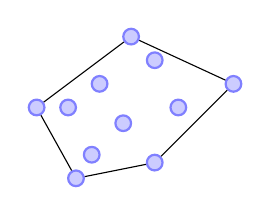
\begin{tikzpicture}[
          n/.style={circle,draw=blue!50,fill=blue!20,thick,inner sep=2pt}
          ]
          \node[n] (a) at (0,1.5)   {};
          \node[n] (b) at (1.2,2.4) {};
          \node[n] (c) at (2.5,1.8) {};
          \node[n] (d) at (1.5,0.8) {};
          \node[n] (e) at (0.5,0.6) {};
          \draw  (a) to (b) to (c) to (d) to (e) to (a);
          \node[n] at (1.5,2.1) {};
          \node[n] at (1.8,1.5) {};
          \node[n] at (1.1,1.3) {};
          \node[n] at (0.4,1.5) {};
          \node[n] at (0.8,1.8) {};
          \node[n] at (0.7,.9) {};
        \end{tikzpicture}       
      \end{column}
      \begin{column}{.75\linewidth}
        \begin{itemize}
        \item Sort points by x-coordinate, then y-coordinate
        \item Add them from left to right into the hull:
          \begin{itemize}
          \item New rightmost point is on the boundary
          \item Adding point to boundary may cause others to be deleted\\
            {\small depending on whether the angle is convex or not}
          \end{itemize}
        \end{itemize}
      \end{column}
    \end{columns}
  \end{block}

  \begin{block}{Huffman codes}
    \begin{itemize}
    \item When storing a text, giving each letter's code the same length wastes
      space
    \item \structure{Example:} $e$ is more common than $q$, so give it a
      shorter code
    \item \structure{Huffman encoding:} Sort letters by frequency, assign codes
      in order
    \end{itemize}
    \begin{columns}
      \begin{column}{.3\linewidth}
        \begin{tabular}{|c|c|l|}\hline
          Char&Freq.&Code\\\hline
          f&5&1100\\
          e&6&1101\\
          c&12&100\\\hline
        \end{tabular}        
      \end{column}
      \begin{column}{.3\linewidth}
        \begin{tabular}{|c|c|l|}\hline
          Char&Freq.&Code\\\hline
          b&13&101\\
          d&16&111\\
          a&45&0\\\hline
        \end{tabular}
      \end{column}
      \begin{column}{.35\linewidth}
        \begin{itemize}
        \item Simple \& fast
        \item Not best compression
        \item Used in JPEG and MP3
        \end{itemize}
      \end{column}
    \end{columns}
  \end{block}
\end{frame}
%%%%%%%%%%%%%%%%%%%%%%%%%%%%%%%%%%%%%%%%%%%%%%%%%%%%%%%%%%%%%%%%%%%%%%%%%%%%%%
\subsubsection{MergeSort}
\begin{frame}{Merge Sort}
  \begin{block}{Recursive sorting}
    \begin{itemize}
    \item Imagine the simpler way to sort recursively a list
    \visible<2->{
    \item[1.] Split your list in two sub-lists\\
      \visible<3->{\small One idea is to split evenly, but not the only one}
    \item[2.] Sort each of them recursively\\
      \visible<3->{\small (base case: size$\leq$1)}
    \item[3.] Merge sorted sublists back\\
      \visible<3->{\small at each step, pick smallest remaining elements of
        sublists, put it after already picked}
    }
    \end{itemize}
  \end{block}

  \begin{columns}
    \begin{column}{.55\linewidth}
      \begin{block}<4->{Merge Sort}
        \begin{itemize}
        \item List splited evenly
        \item Sub-list copied away
        \item Merge trivial
        \end{itemize}        
        (invented by John von Neumann in 1945)
      \end{block}      
    \end{column}
    \begin{column}{.4\linewidth}
      \visible<4->{\includegraphics{fig/sort_merge.fig}}
    \end{column}
  \end{columns}
\end{frame}
%%%%%%%%%%%%%%%%%%%%%%%%%%%%%%%%%%%%%%%%%%%%%%%%%%%%%%%%%%%%%%%%%%%%%%%%%% 
\begin{frame}[fragile]{Merge Sort}
  \begin{block}{Scala code}\smallskip
    \begin{columns}
      \begin{column}{.45\linewidth}
        \begin{boitecode}{}
def mergeSort(m: List[Int]):List[Int] =\{
  \structure{// short enought to be already sorted}
  if (m.length <= 1) 
    return m

  \structure{// Slice (=cut) the array in two parts}
  val middle = m.length / 2
  val left  = m.slice(0,middle)
  val right = m.slice(middle,m.length)
  
  \structure{// Sort each parts}
  val leftSorted  = mergeSort(left)
  val rightSorted = mergeSort(right)

  \structure{// Merge them back}
  return merge(leftSorted, rightSorted)
\}          
        \end{boitecode}
%        \vspace{-.8\baselineskip}{\tiny~~ (C) Wikipedia}
      \end{column}
      \begin{column}{.4\linewidth}
        \begin{boitecode}{}
def merge(xs:List[Int], ys:List[Int]) 
    :List[Int] = \{

  (xs,ys) match \{

    case ( _ , Nil) => xs
    case (Nil,  _ ) => ys

    case (x::x2, y::y2) =>
       if (x < y) \{
          x :: merge(x2 , ys)
       \} else \{
          y :: merge(xs , y2)
       \}
  \}
\}
        \end{boitecode}
      \end{column}
    \end{columns}
  \end{block}
  \begin{block}{Complexity Analysis}
    \begin{itemize}
    \item \structure{Time:} $\log(n)$ recursive calls, each of them being
      linear $\leadsto \alert{\Theta(n\times \log(n))}$
    \item \structure{Space:} Need to copy the array $\leadsto 2n$ (quite
      annoying) + $log(n)$ for the stack
    \end{itemize}
  \end{block}
\end{frame}
%%%%%%%%%%%%%%%%%%%%%%%%%%%%%%%%%%%%%%%%%%%%%%%%%%%%%%%%%%%%%%%%%%%%%%%%%% 
\subsubsection{QuickSort}
%%%%%%%%%%%%%%%%%%%%%%%%%%%%%%%%%%%%%%%%%%%%%%%%%%%%%%%%%%%%%%%%%%%%%%%%%% 
\begin{frame}{QuickSort}

  \begin{block}{Presentation}
    \begin{itemize}
    \item Invented by C.A.R. Hoare in 1962
    \item Widely used (in C library for example)
    \end{itemize}
  \end{block}

  \begin{block}{Big lines}
    \begin{itemize}
    \item Pick one element, called \alert{\textit{pivot}}
      (random is ok)
    \item Reorder elements so that:
      \begin{minipage}{.55\linewidth}
        \begin{itemize}
        \item elements smaller to the pivot are before it%
          \vspace{-.4\baselineskip}
        \item elements larger to the pivot are after it
        \end{itemize}
      \end{minipage}
    \item Recursively sort the parts before and after the pivot
    \end{itemize}
  \end{block}

  \begin{block}{Questions to answer}
    \begin{itemize}
    \item How to pick the pivot? (random is ok)
    \item How to reorder the elements?
      \begin{itemize}
      \item \structure{First solution:} build sub-list (but this requires extra
        space)
      \item \structure{Other solution:} invert in place (but hinders stability,
        see below)
      \end{itemize}
    \end{itemize}
  \end{block}
\end{frame}
%%%%%%%%%%%%%%%%%%%%%%%%%%%%%%%%%%%%%%%%%%%%%%%%%%%%%%%%%%%%%%%%%%%%%%%%%% 
\begin{frame}[fragile]{Simple Quick Sort}
  \begin{columns}
    \begin{column}{.44\linewidth}
      \begin{block}{It's easy with sub-lists:}
        \begin{itemize}
        \item Create two empty list variables
        \item Iterate over the original list;
          copy elements in correct sublist
        \item Recurse
        \item Concatenate results
        \end{itemize}
      \end{block}
    \end{column}
    \begin{column}{.55\linewidth}
    \begin{boitecode}{}
def quicksort(lst:List[Int]):List[Int] = \{
  if (lst.length <= 1) \structure{// Base case}
    return lst
  
  \structure{// Randomly pick a pivot value}
  val pivot = lst(lst.length / 2)      

  \structure{// split the list}
  var lows: List[Int] = Nil
  var mids: List[Int] = Nil
  var highs: List[Int] = Nil
  for (item <- lst) \{ \structure{// classify the items}
    if ( item == pivot)    \{ mids  = item :: mids \}
    else if (item < pivot) \{ lows  = item :: lows \}
    else                   \{ highs = item :: highs\}
  \}

  \structure{// return sorted list appending chunks}
  quicksort(lows) ::: mids ::: quicksort(highs) 
\}      
    \end{boitecode}      
    \end{column}
  \end{columns}

  \begin{block}{Problem}
    \begin{itemize}
    \item Space complexity is about $2n+\log(n))$...\\
      {\small (2n for array duplication, log(n) for the recursion stack)}
    \end{itemize}
  \end{block}
\end{frame}
%%%%%%%%%%%%%%%%%%%%%%%%%%%%%%%%%%%%%%%%%%%%%%%%%%%%%%%%%%%%%%%%%%%%%%%%%% 
\begin{frame}[fragile]{In-place Quick Sort}
  \null\vspace{-2.3\baselineskip}
  \begin{columns}
    \begin{column}{.6\linewidth}
      \begin{block}{Big lines of the list reordering}
        \begin{itemize}
        \item Put the pivot at the end
        \item Traverse the list
          \begin{itemize}
          \item If visited element is larger, do nothing
          \item Else swap with ``storage point'' \\
            + shift storage right
          \item[] (storage point is on left initially)
          \end{itemize}
        \item Swap pivot with storage point
        \end{itemize}
      \end{block}      
    \end{column}
    \begin{column}{.4\linewidth}
      \includegraphics{fig/sort_qsort.fig}      
    \end{column}
  \end{columns}\vspace{-\baselineskip}

  \begin{center}
    \begin{boitecode}{}
def quicksort(array:Array[Int]) \{
  def lambda(array:Array[Int], left:Int, right:Int, pivotIndex:Int) \{
    val pivotValue = array(pivotIndex)
    array.swap(pivotIndex, right) \structure{// Move pivot to end (swap() does not exist)}
    val storeIndex = left
    for (i <- left to right-1) \{
      if (array(i) <= pivotValue) \{
        array.swap(i, storeIndex)
        storeIndex = storeIndex + 1
    \} \}
    array.swap(storeIndex, right) \structure{// Move pivot to its final place}
    lambda(array, left, pivotIndex, (pivotIndex-left)/2)
    lambda(array, pivotIndex, right, (right-pivotIndex)/2)
  \}
  lambda(array, 0, array.length-1, array.length/2)
\}
  \end{boitecode}
 \end{center}
\end{frame}
%%%%%%%%%%%%%%%%%%%%%%%%%%%%%%%%%%%%%%%%%%%%%%%%%%%%%%%%%%%%%%%%%%%%%%%%%%%%%
\begin{frame}{In-place QuickSort Complexity (1/2)}
  
  \begin{block}{Best case for divide-and-conquer algorithms: \alert{Even Split}}
    \begin{itemize}
    \item Split the amount of work by 2 at each step (thus $\Theta(log(n))$
      recursive calls)
    \item Work on each subproblem linear with its size (thus each call in
      $\Theta(n)$)
    \end{itemize}
  \end{block}

  \begin{block}{The recursion tree for best case:}\medskip
    \centerline{
      \includegraphics[width=.7\linewidth]{fig/algo_quick_bestcase.fig}
    }
  \end{block}

  \begin{block}{What if we split 1\%/99\% at each step (instead of 50\%/50\%)?}
    \begin{itemize}
    \item We get \visible<2->{$100\times\log(n)$} steps 
          $\leadsto$ whole algorithm in \visible<3->{$\Theta(n\log(n))$}
    \end{itemize}
  \end{block}
\end{frame}
%%%%%%%%%%%%%%%%%%%%%%%%%%%%%%%%%%%%%%%%%%%%%%%%%%%%%%%%%%%%%%%%%%%%%%%%%%%%%
\begin{frame}{In-place QuickSort Complexity (2/2)}
  \begin{block}{What if we have a fixed amount on one side?}
    \begin{itemize}
    \item (happens when every values are duplicated, or with the wrong pivot)

    \centerline{
      \includegraphics[width=.6\linewidth]{fig/algo_quick_worstcase.fig}
    }
    \item We get \visible<2->{$O(n)$} steps 
      $\leadsto$ whole algorithm in \visible<3->{\alert{$O(n^2)$}} in worst case
    \end{itemize}    
  \end{block}\vspace{-.4\baselineskip}

  \begin{block}{That's a fairly bad worst case time}
    \begin{itemize}
    \item Worst than MergeSort, for example
    \item But called Quicksort anyway because faster \textit{in practice}
      than MergeSort% and HeapSort
    \item In-Place version of both algorithms are \alert{not stable}
    \item Both can be quite easily parallelized
    \item \structure{Space complexity:}
      $O(\log(n))$ (to store the recursion stack)
    \end{itemize}
  \end{block}\vspace{-\baselineskip}

  \begin{flushright}
    (this ends the second lecture)    
  \end{flushright}
\end{frame}
%%%%%%%%%%%%%%%%%%%%%%%%%%%%%%%%%%%%%%%%%%%%%%%%%%%%%%%%%%%%%%%%%%%%%%%%%%%%%%

%%% Local Variables:
%%% coding: utf-8

%\part{Correction of Software Systems}\mypartpage
%%%%%%%%%%%%%%%%%%%%%%%%%%%%%%%%%%%%%%%%%%%%%%%%%%%%%%%%%%%%%%%%%%%%%%%%%% 
\section{Introduction}
\begin{frame}{Sorting Algorithm Performance Discussion}
  \begin{block}<+->{We have shown that}\medskip

    \begin{tabular}{|l|c|c|c|c|}\cline{2-5}
      \multicolumn{1}{}{}&
        \multicolumn{3}{|c|}{\structure{Amount of comparisons}}&
        \structure{Memory}\\\cline{2-4}
      \multicolumn{1}{c|}{}&\structure{Best Case}&
        \structure{Average Case}&\structure{Worst Case}&
        \structure{Complexity}\\\hline

      Selection Sort&$O(n^2)$&$O(n^2)$&$O(n^2)$&$\Theta(1)$\\\hline
      Insertion Sort&$O(n)$&$O(n^2)$&$O(n^2)$&$\Theta(1)$\\\hline
      Bubble Sort&$O(n)$&$O(n^2)$&$O(n^2)$&$\Theta(1)$\\\hline 

      \hline
      Quick Sort&$O(n\log(n))$&$O(n\log(n))$&$O(n^2)$&$O(\log(n))$\\\hline
      Merge Sort&$O(n\log(n))$&$O(n\log(n))$&$O(n\log(n))$&$O(n)$\\\hline      
    \end{tabular}

    \begin{itemize}
    \item Very accurate knowledge on achieved performance
    \end{itemize}
  \end{block}

  \visible<+->{
  \concept{But wait a second\ldots}
  
  \begin{block}{How do you know this code actually sorts the array?}
    \begin{itemize}
    \item Because you see it, it's obvious (yeah, right\ldots)
    \item Because the teacher / a friend says so
    \item Because it's written in a book / on the Internet
    \item Because you tested it
    \end{itemize}
  \end{block}
}
\end{frame}  
%%%%%%%%%%%%%%%%%%%%%%%%%%%%%%%%%%%%%%%%%%%%%%%%%%%%%%%%%%%%%%%%%%%%%%%%%%%%
\begin{frame}{Because it's obvious you said?}
  \begin{block}{Let's consider the following problem}
    \begin{itemize}
    \item You have a robot arm equipped with a soldering iron (for example)
    \item You have several positions were the arm should do its soldering job
    \item You must decide the order in which the arm visit the positions
    \item You want to minimize the time (ie travel distance) it takes to visit
      all positions
    \end{itemize}
  \end{block}

  \centerline{\includegraphics[width=.6\linewidth]{fig/proof_salesman1.fig}}
\end{frame}
%%%%%%%%%%%%%%%%%%%%%%%%%%%%%%%%%%%%%%%%%%%%%%%%%%%%%%%%%%%%%%%%%%%%%%%%%%%%%%
\begin{frame}{Nearest Neighbor Tour}
  \begin{block}{Here is a very popular algorithm to that problem}
    \begin{itemize}
    \item Pick and visit an initial point $p_0$, and let $i=0$
    \item While there are still unvisited points
      \begin{itemize}
      \item $i=i+1$
      \item let $p_i$ be the closest unvisited point to $p_{i-1}$
      \item Visit $p_i$
      \end{itemize}
    \item Return to $p_0$ from $p_i$
    \end{itemize}
  \end{block}

  \begin{block}{Advantage of that algorithm}
    \begin{itemize}
    \item It is simple to understand and implement; It's very efficient: $O(n)$
    \end{itemize}
  \end{block}
  
  \begin{alertblock}<2->{\only<2->{But it is not correct!}}
    \begin{minipage}{.6\linewidth}
      \only<1| handout:0>{\includegraphics[width=\linewidth,subfig=1]{fig/proof_salesman2.fig}}%
      \only<2| handout:0>{\includegraphics[width=\linewidth,subfig=2]{fig/proof_salesman2.fig}}%
      \only<3->{\includegraphics[width=\linewidth,subfig=3]{fig/proof_salesman2.fig}}%      
    \end{minipage}\hfill
    \begin{minipage}{.35\linewidth}
      \begin{center}
        \only<4>{Choosing carefully $p_0$\\
          (left-most or whatever) \\
          \alert{will \textbf{not} help}}        
      \end{center}
    \end{minipage}
  \end{alertblock}
\end{frame}
%%%%%%%%%%%%%%%%%%%%%%%%%%%%%%%%%%%%%%%%%%%%%%%%%%%%%%%%%%%%%%%%%%%%%%%%%% 
\begin{frame}{Closest Pair Tour}
  \begin{block}{Let's try to fix our algorithm}
    \begin{itemize}
    \item Walking to the closest point seems too restrictive: 
      {\small traps into unwanted moves}
    \item Let's repeatedly connect the closest pairs 
      {\small(w/o forming cycles or 3ways branches)}
    \end{itemize}
  \end{block}\vspace{-.8\baselineskip}

  \begin{block}{The algorithm}
    \begin{itemize}
    \item Let $n$ be the number of points in the set 
    \item For $i=1$ to $n-1$ do
      \begin{itemize}
      \item Let $d=\infty$
      \item For each pair of endpoints $(x,y)$ of partial paths
        \begin{itemize}
        \item If $dist(x,y)\leq d$ then $x_m=x$, $y_m=y$, $d=dist(x,y)$
        \end{itemize}
      \item Connect $(x_m,y_m)$ by an edge
      \end{itemize}
    \item Connect the two endpoints by an edge
    \end{itemize}
  \end{block}\vspace{-.7\baselineskip}

  \begin{block}{Works correctly for previous data\only<2->{, \alert{but still
          not correct}}}\medskip
    \begin{center}
      \only<1-2| handout:0>{\includegraphics[width=.6\linewidth,subfig=1]{fig/proof_salesman3.fig}}%
      \only<3| handout:0>{\includegraphics[width=.6\linewidth,subfig=2]{fig/proof_salesman3.fig}}%
      \only<4->{\includegraphics[width=.6\linewidth,subfig=3]{fig/proof_salesman3.fig}}%      
      
    \end{center}    
  \end{block}
\end{frame}
%%%%%%%%%%%%%%%%%%%%%%%%%%%%%%%%%%%%%%%%%%%%%%%%%%%%%%%%%%%%%%%%%%%%%%%%%% 
\begin{frame}{That's the Traveling Salesman Problem}
  \begin{block}{A correct algorithm}
    \begin{itemize}
    \item $d=\infty$
    \item For each permutation $\Pi_i$ of the $n!$ existing ones
      \begin{itemize}
      \item if ($cost(\Pi_i)\leq d$) then
        \begin{itemize}
        \item $d=cost(\Pi_i)$ and $P_{min}=\Pi_i$
        \end{itemize}
      \end{itemize}
    \item return $P_i$
    \end{itemize}
  \end{block}

  \begin{block}{Actually no known correct and polynomial algorithm}
    \begin{itemize}
    \item This algorithm is very slow (exponential time)
    \item But that's the only correct known
    \item (this problem is one of the NP-Complete set, by the way)
    \end{itemize}
  \end{block}

  \bigskip
  \concept{Conclusion: never trust ``obviously correct'' algorithms}
\end{frame}
%%%%%%%%%%%%%%%%%%%%%%%%%%%%%%%%%%%%%%%%%%%%%%%%%%%%%%%%%%%%%%%%%%%%%%%%%% 
\begin{frame}{Other try to convince septics: \alert{you test it}}
  \begin{block}{Issues} 
    \begin{itemize}
    \item a \textit{whole} load of arrays exists out there. Cannot test them
      all\ldots
     \item How much should you test to get convincing?
       Which ones do you pick?
   \end{itemize}
  \end{block}

  \begin{block}{Let's look at another (simpler) problem}
    \begin{itemize}
    \item \structure{Input:} 3 integers values, representing the sides'
      length of a triangle
    \item \structure{Output:} Tells whether the triangle is
      \begin{itemize}
      \item \structure{Scalene:} no two sides are equal
      \item \structure{Isosceles:} exactly two sides are equal
      \item \structure{Equilateral:} all sides are equal
      \end{itemize}
    \end{itemize}
  \end{block}

  \begin{alertblock}{Quiz: Create a set of Test Cases for this program}
    \begin{itemize}
    \item Ie, the list of tests you need to write to ensure that the program is robust
    \end{itemize}
  \end{alertblock}
\end{frame}
%%%%%%%%%%%%%%%%%%%%%%%%%%%%%%%%%%%%%%%%%%%%%%%%%%%%%%%%%%%%%%%%%%%%%%%%%% 
\begin{frame}[squeeze]{Solutions -- 1 point for each correct answer}
  \begin{itemize}
  \item T1: \trou{(4,1,2): Invalid triangle (because $(a,b,c)$ with $a>b+c$)%
      \hbox to 2cm{\vbox to.6\baselineskip{\includegraphics[scale=.5]{fig/proof_triangle1.fig}}}}%
  \item T2: \trou{Permutations of the previous: $(1,2,4)$, $(2,1,4)$~~~~~~~~~~~~~~~~~~~~~~~~~~~~~~~}
    \trou{$\leadsto$ valid iff $a\leq b+c$ 
      \textbf{and $\mathbf{b\leq a+c}$ and $\mathbf{c\leq a+b}$} ~~~~~~~~~~~~~~~~~~~~~~~~~~~~~~} 
  \item T3: \trou{Invalid with equal sum: $(4,2,2)$ $\leadsto$ need to use $<$
      instead of $\leq$~~~~~~~~~~~}
  \item T4: \trou{Permutations of the previous: $(2,4,2)$, $(2,2,4)$~~~~~~~~~~~~~~~~~~~~~~~~~~~~~~~}
  \item T5: \trou{A valid scalene triangle: $(3,4,5)$~~~~~~~~~~~~~~~~~~~~~~~~~~~~~~~~~~~~~~~~~~~~~~~~}
  \item T6: \trou{A valid equilateral triangle: $(3,3,3)$~~~~~~~~~~~~~~~~~~~~~~~~~~~~~~~~~~~~~~~~~~~~}
  \item T7: \trou{A valid isoceles triangle: $(3,4,3)$~~~~~~~~~~~~~~~~~~~~~~~~~~~~~~~~~~~~~~~~~~~~~~~}
  \item T8: \trou{All permutations of isoceles triangle: $(4,3,3)$,$(3,3,4)$~~~~~~~~~~~~~~~~~~~~~~}
  \item T9: \trou{One side with \textbf{zero} value: $(0,4,3)$~~~~~~~~~~~~~~~~~~~~~~~~~~~~~~~~~~~~~~~~~~~~}
  \item T10: \trou{One side with \textbf{negative} value: $(-1,4,3)$~~~~~~~~~~~~~~~~~~~~~~~~~~~~~~~~~~~~}
  \item T11: \trou{All sides with \textbf{zero} values: $(0,0,0)$~~~~~~~~~~~~~~~~~~~~~~~~~~~~~~~~~~~~~~~~~~~}
  \item T12: \trou{At least one side non-integer: $(1,3,2.6)$ or even $(1,2,a)$~~~~~~~~~~~~~~~~~}
  \item T13: \trou{Wrong number of arguments: $(2,4)$ or $(1,2,2,5)$~~~~~~~~~~~~~~~~~~~~~~~~~~}
  \end{itemize}
\end{frame}
%%%%%%%%%%%%%%%%%%%%%%%%%%%%%%%%%%%%%%%%%%%%%%%%%%%%%%%%%%%%%%%%%%%%%%%%%%%%
\begin{frame}{First Conclusions on Testing}
  \begin{block}{About the Quiz}
    \begin{itemize}
    \item All T1-T13 correspond to failures actually found in some implementations
    \item How many tests did you found yourself?\\
      $<5$? ~~ $5-7$? ~~ $8-10$? ~~ $>10$? ~~ All?
    \item Highly qualified, experienced programmers score \alert{7.8} on average
    \end{itemize}
  \end{block}
  \begin{block}{Testing aint easy}
    \begin{itemize}
    \item Finding good and sufficiently many test cases is difficult
    \item Even a good set of test cases cannot exclude \alert{all} failures
    \item Without a specification, it is not clear even what a failure
      \alert{is} 
    \end{itemize}
  \end{block}
\end{frame}
%%%%%%%%%%%%%%%%%%%%%%%%%%%%%%%%%%%%%%%%%%%%%%%%%%%%%%%%%%%%%%%%%%%%%%%%%%%%%
\begin{frame}{Stop academic examples, check Real Life!}
  \begin{block}{Cost of Software Errors: some numbers}
    \begin{itemize}
    \item \structure{\$60 billion}: Estimated cost of software errors for US
      economy per year [2002]
    \item \structure{\$240 billion}: Size of US software industry [2002]\\
      {\small incl. profit, sales, marketing, development (50\% maybe)}
    \item \structure{50\%}: estimated part of each software project spent on
      testing\\ 
      {\small(spans from 30\% to 80\%)}

    \item Rough estimate: \structure{money spent on testing $\approx$ cost of
        remaining errors}
    \item That's \alert{50\% of size of software industry!}
    \end{itemize}
  \end{block}

 \begin{block}{More on Testing in POO lecture, in january}
   \begin{itemize}
   \item We need \structure{systematic}, \structure{efficient}, \structure{tool
       supported} \alert{testing} and \alert{debugging} methods
   \end{itemize}
 \end{block}
  
 \begin{block}{To convince real septics, you have to \textbf{prove} correctness}
   \begin{itemize}
   \item And you cannot do that without a proper specification (at least)
   \end{itemize}
 \end{block}
\end{frame}
%%%%%%%%%%%%%%%%%%%%%%%%%%%%%%%%%%%%%%%%%%%%%%%%%%%%%%%%%%%%%%%%%%%%%%%%%% 
\section{Specification}\sectionpage
\begin{frame}{How to prove that 'selection sort' sorts arrays?}
  \begin{block}{Back to the roots: what exactly do you want to prove?}
    \begin{itemize}
    \item Proper specification mandatory to proof: gives what we have, what we
      want
    \item We also need a mathematical logic to carry the proof
    \end{itemize}
  \end{block}

  \begin{block}{Hoare Logic {\normalsize[Hoare 1969]}}
    \begin{itemize}
    \item Set of logical rules to reason about the correctness of computer
      programs
    \item \structure{Central feature:} description of state changes induced by
      code execution
    \item \alert{\textbf{Hoare triple:}} \framebox{$\{P\}~ C ~\{Q\}$}
      \begin{itemize}
      \item C is the code to be run
      \item P is the \alert{\textbf{precondition}}
        (assertion about previous state)
      \item Q is the \alert{\textbf{postcondition}}
        (assertion about next state)
      \item This can be read as ``If P is true, then when I run C, Q becomes
        true''
      \item C is said to satisfy specification $(P,Q)$
      \end{itemize}
    \item Such notation allows very precise algorithm specifications
    \item Axioms and Inference rules allow rigorous correctness demonstrations
      \smallskip
    \item \structure{Note:} other logics (temporal logic) proposed as
      replacement, but harder
    \end{itemize}
  \end{block}
\end{frame}
%%%%%%%%%%%%%%%%%%%%%%%%%%%%%%%%%%%%%%%%%%%%%%%%%%%%%%%%%%%%%%%%%%%%%%%%%%%%%%
\begin{frame}{Introducing (bad) joke about precise specification}
  \begin{block}{While traversing Scotland, 3 people see a cow}\medskip
    \begin{columns}
      \begin{column}{.55\linewidth}
        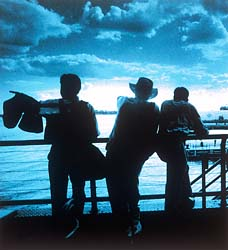
\includegraphics[width=.3\linewidth]{img/proof_guys.png}\hfill
        
\includegraphics[width=.6\linewidth]{img/proof_scotland.png}
        
        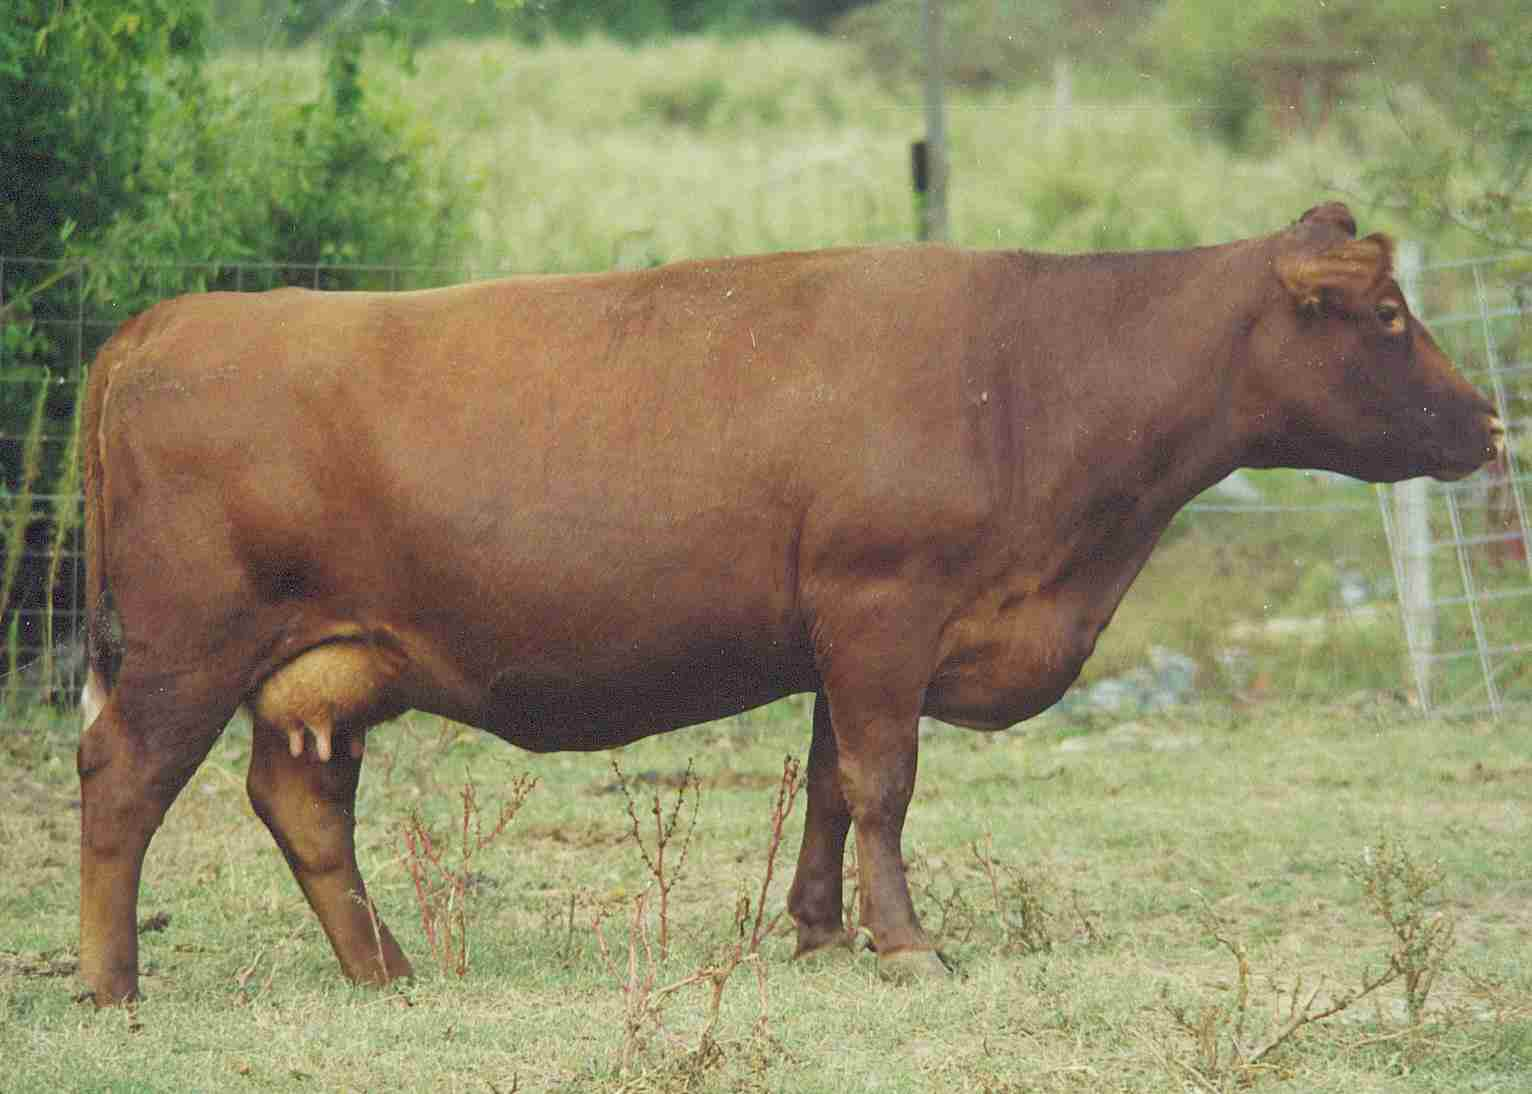
\includegraphics[width=\linewidth]{img/proof_cow.png}
      \end{column}

      \begin{column}{.45\linewidth}
        \begin{block}<2->{The Economist says:}
          \begin{itemize}
          \item Cows in Scotland are brown
          \end{itemize}
        \end{block}

        \begin{block}<3->{The Logician says:}
          \begin{itemize}
          \item No, no. There are cows in Scotland of which one is brown
          \end{itemize}
        \end{block}

        \begin{block}<4->{The Computer Scientist says:}
          \begin{itemize}
          \item No, no. There is at least one cow in Scotland of which one
            side is brown
          \end{itemize}
        \end{block}
      \end{column}
    \end{columns}
  \end{block}
\end{frame}
%%%%%%%%%%%%%%%%%%%%%%%%%%%%%%%%%%%%%%%%%%%%%%%%%%%%%%%%%%%%%%%%%%%%%%%%%%
\begin{frame}[squeeze]{Specification: Putting it into Practice}
  \begin{block}{Back to our Example: A sorting program}\smallskip
    \texttt{def sort(a:Array[Int]):Array[Int] = \{ \ldots\ \}}
  \end{block}\vspace{-.3\baselineskip}
  \begin{block}{Specification \only<4->{V1}}
    \begin{itemize}\vspace{-.2\baselineskip}
    \item \structure{Precondition}: $a$ is an array
    \item \structure{Post-condition}: returns the sorted argument array
    \item<2-> \alert{Is it good enough?}
      \only<3->{
         \alert{Not quite:} 
         \texttt{sort(\{2,1,2\} $\leadsto$ \{1,2,2,17\}} ~\Frownie}
    \end{itemize}
  \end{block}\vspace{-.8\baselineskip}
  \begin{block}<4->{Specification V2}
    \begin{itemize}\vspace{-.2\baselineskip}
    \item \structure{Precondition}: $a$ is an array
    \item \structure{Post-condition}: returns a sorted array \alert{with only
        elements} of $a$
    \item<5->[\Frownie] \texttt{sort(\{3,2,1\} $\leadsto$ \{2,2,2,2,2\}}
    \end{itemize}
  \end{block}\vspace{-.8\baselineskip}
  \begin{block}<6->{Specification V3}
    \begin{itemize}\vspace{-.2\baselineskip}
    \item \structure{Precondition}: $a$ is an array
    \item \structure{Post-condition}: returns a \alert{permutation} of $a$ that
      is sorted
    \item<7->[\Frownie] \texttt{sort(\{\})} leads to unwanted behavior
    \end{itemize}
  \end{block}\vspace{-.8\baselineskip}
  \begin{block}<8->{Specification V4}
    \begin{itemize}\vspace{-.2\baselineskip}
    \item \structure{Precondition}: $a$ is a \alert{non-null} array
    \item \structure{Post-condition}: returns a permutation of $a$ that
      is sorted
    \end{itemize}
  \end{block}
\end{frame}
%%%%%%%%%%%%%%%%%%%%%%%%%%%%%%%%%%%%%%%%%%%%%%%%%%%%%%%%%%%%%%%%%%%%%%%%%% 
\begin{frame}{The Contract Metaphor}
  \begin{boitequote}{B. Meyer, Computer 25(10)40-51, 1992}
    \hspace{-1.5em}\alert{Contract} is preferred specification metaphor for
    procedural and OO.
  \end{boitequote}\bigskip

  \begin{block}{Same Principles as \alert{Legal Contract} between a Client and
      Supplier}
    \begin{description}
    \item[Supplier] aka Implementer, in Java, a class or method
    \item[Client] Mostly a caller object, or human user for main()
    \item[Contract] One or more pairs of ensures/requires clauses\\
           defining mutual obligations of client and implementer
    \end{description}
  \end{block}

  \begin{block}{Meaning of a Contract: Specification of method \texttt{C@m()}}
    \begin{itemize}
    \item "If a caller of \texttt{C@m()} fulfills the \alert{required
        Precondition},\\ then the class \texttt{C} \alert{ensures} that the
      \alert{Postcondition} holds after \texttt{m()} finishes."
    \end{itemize}
  \end{block}
  \begin{block}{Wrong Interpretations:}
    \begin{itemize}
    \item "Any caller of C@m() must fulfill the required Precondition."
    \item "Whenever the required Precondition holds, then C@m() is executed."
    \end{itemize}
  \end{block}
\end{frame}
%%%%%%%%%%%%%%%%%%%%%%%%%%%%%%%%%%%%%%%%%%%%%%%%%%%%%%%%%%%%%%%%%%%%%%%%%%
\begin{frame}{What is Design By Contract?}
  \begin{boitequote}{}
    View the relationship between two classes as a formal agreement, expressing
    each party's rights and obligations.~\hfill{\rm -- Bertrand Meyer}
  \end{boitequote}

  \begin{block}{Example: Airline Reservation}
    \begin{tabular}{p{.15\linewidth}|p{.37\linewidth}|p{.37\linewidth}}\hline
      &Obligations&Rights\\\hline
      Customer&
      \begin{itemize}\vspace{-.8\baselineskip}
      \item Be at Paris airport at least 3 hour before scheduled departure time
      \item Bring acceptable baggage
      \item Pay ticket price
      \end{itemize}\vspace{-1.2\baselineskip}
      &
      \begin{itemize}\vspace{-.8\baselineskip}
      \item Reach Los Angeles
      \end{itemize}
      \\\hline
      Airline&
      \begin{itemize}\vspace{-.8\baselineskip}
      \item Bring customer to Los Angeles
      \end{itemize}
      &
      \begin{itemize}\vspace{-.8\baselineskip}
      \item No need to carry passenger who is late
      \item has unacceptable baggage
      \item or without paid ticket
      \end{itemize}\vspace{-1.2\baselineskip}
    \end{tabular}
  \end{block}
  \begin{itemize}
  \item Each party expects benefits (rights) and accepts obligations
  \item Usually, one party's benefits are the other party's obligations
  \item Contract is declarative: it is described so that both parties can
    understand \textit{what} service will be guaranteed without saying
    \textit{how}
  \end{itemize}
\end{frame}
%%%%%%%%%%%%%%%%%%%%%%%%%%%%%%%%%%%%%%%%%%%%%%%%%%%%%%%%%%%%%%%%%%%%%%%%%% 
\begin{frame}{Testing \textit{vs.} Verification}
  \begin{block}{Testing}
    \begin{itemize}
    \item \structure{Goal:} find evidence for \alert{presence} of failures
    \item \alert{Testing means to execute a program with the \textbf{intent of
          detecting failure}}
    \item \structure{Related techniques:}  code reviews, program inspections
    \item Automatize the testing process is delayed until the POO module
    \end{itemize}
  \end{block}

  \begin{block}{Verification}
    \begin{itemize}
    \item \structure{Goal:} find evidence for \alert{absence} of failures
    \item \alert{Testing cannot guarantee correctness, i.e., absence of
        failures}
    \item \structure{Related techniques:} code generation, program synthesis
      (from spec)
    \item<2->\alert{This week:} How can we prove the correctness of an algorithm?
    \end{itemize}
  \end{block}

  \begin{block}{Debugging}
    \begin{itemize}
    \item Systematic process to find and eliminate defects leading to
      observed failures
    \end{itemize}
  \end{block}
\end{frame}
%%%%%%%%%%%%%%%%%%%%%%%%%%%%%%%%%%%%%%%%%%%%%%%%%%%%%%%%%%%%%%%%%%%%%%%%%% 
\section{Hoare Logic}\sectionpage
%%%%%%%%%%%%%%%%%%%%%%%%%%%%%%%%%%%%%%%%%%%%%%%%%%%%%%%%%%%%%%%%%%%%%%%%%% 
\begin{frame}{Back on Hoare Logic}
  \begin{block}{Hoare Logic {\normalsize[Hoare 1969]}}
    \begin{itemize}
    \item Set of logical rules to reason about the correctness of computer
      programs
    \item \structure{Central feature:} description of state changes induced by
      code execution
    \item \alert{\textbf{Hoare triple:}} \framebox{$\{P\}~ C ~\{Q\}$}
      \begin{itemize}
      \item C is the code to be run
      \item P is the \alert{\textbf{precondition}}
        (assertion about previous state)
      \item Q is the \alert{\textbf{postcondition}}
        (assertion about next state)
      \item This can be read as ``If P is true, then when I run C, Q becomes
        true''
      \item C is said to satisfy specification $(P,Q)$
      \end{itemize}
    \item Such notation allows very precise algorithm specifications
    \item Axioms and Inference rules allow rigorous correctness demonstrations
      \smallskip
    \item \structure{Note:} other logics (temporal logic) proposed as
      replacement, but harder
    \end{itemize}
  \end{block}
  
  \begin{alertblock}{Game now}
    \begin{itemize}
    \item See how we can \textbf{prove} that a Hoare triple holds
    \end{itemize}    
  \end{alertblock}
\end{frame}
%%%%%%%%%%%%%%%%%%%%%%%%%%%%%%%%%%%%%%%%%%%%%%%%%%%%%%%%%%%%%%%%%%%%%%%%%% 
\begin{frame}{Assertions}
  \concept{What exactly is an assertion?}

  \begin{block}{Definition}\medskip
    Formula of first order logic describing relationships between algorithm's
    variables
  \end{block}

  \begin{block}{Constituted of:}
    \begin{itemize}
    \item \structure{Variables} of algorithm pseudo-code
    \item \structure{Logical connectors:} $\wedge$ (and) $\vee$ (or) $\neg$
      (not) $\Rightarrow$, $\Leftarrow$
    \item \structure{Quantifiers:} $\exists$ (exists), $\forall$ (for all)
    \item \structure{Value-specific elements} (describing integers, reals,
      booleans, arrays, sets, \ldots)
    \end{itemize}
  \end{block}

  \begin{block}{Example:}
    \begin{itemize}
    \item $(x\times y = z) ~\wedge~ (x\leq 0)$
    \item $n^2\geq x$
    \end{itemize}
  \end{block}
\end{frame}
%%%%%%%%%%%%%%%%%%%%%%%%%%%%%%%%%%%%%%%%%%%%%%%%%%%%%%%%%%%%%%%%%%%%%%%%%% 
\begin{frame}{Examples of specification}

  \begin{block}{Solving quadratic equations ($ax^2+bx+c=0$)}
    \begin{description}
    \item[P:] $a,b,c \in\mathbb{R}$ and $a\neq 0$
    \item[Q:] $(solAmount\in\mathbb{N}) \wedge (s,t \in\mathbb{R}) \wedge$\\
      ~~~$(~(solAmount = 0) \vee$\\
      ~~~~~$(solAmount = 1 \wedge as^2+bs+c=0) \vee$\\
      ~~~~~$(solAmount = 2 \wedge as^2+bs+c=0 \wedge at^2+bt+c=0 \wedge s\neq t)
      )$     
    \end{description}
  \end{block}

  \begin{block}{Possible implementation}
    
  \end{block}
  \begin{columns}
    \begin{column}{.4\linewidth}
  \framebox{
    \begin{minipage}{\linewidth}      
      $\Delta=b^2-4ac$\\
      if ($\Delta>0$) \\
      \null~~$s=\frac{-b+\sqrt{\Delta}}{2a}; t=\frac{-b-\sqrt{\Delta}}{2a};$\\
      \null~~$solAmount=2$\\
      else if ($\Delta=0$) \\
      \null~~$s=\frac{-b}{2a}; solAmount=1$\\
      else (ie, $\Delta<0$)\\
      \null~~solAmount=0
  \end{minipage}}      
    \end{column}

    \begin{column}{.5\linewidth}
      \begin{itemize}
      \item Here, the proof will be difficult\ldots
      \item \ldots because it is trivial.
      \item Correctness comes from definitions!
      \end{itemize}
    \end{column}
  \end{columns}
\end{frame}
%%%%%%%%%%%%%%%%%%%%%%%%%%%%%%%%%%%%%%%%%%%%%%%%%%%%%%%%%%%%%%%%%%%%%%%%%% 
\begin{frame}{Demonstration tool: inference rules}
  \begin{block}{Definitions}
    \begin{itemize}
    \item \structure{Inference:} deducting new facts by combining existing
      facts correctly
    \item \structure{Inference rule:} mechanism specifying how facts can be
      combined
    \end{itemize}
  \end{block}

  \begin{block}{Classical representation of each rule:}
    $$\frac{p_1, p_2, p_3, \ldots, p_n}{q}$$
    \begin{itemize}
    \item Can be read as ``if all $p_1, p_2, p_3, \ldots, p_n$ are true, then
      $q$ is also true''
    \item Or ``in order to prove $q$, you have to prove $p_1, p_2, p_3, \ldots,
      p_n$'' 
    \item Or ``$q$ can be deduced from $p_1, p_2, p_3, \ldots, p_n$''
    \end{itemize}
  \end{block}
\end{frame}
%%%%%%%%%%%%%%%%%%%%%%%%%%%%%%%%%%%%%%%%%%%%%%%%%%%%%%%%%%%%%%%%%%%%%%%%%% 
\begin{frame}{First axioms and rules}
  \begin{block}{Empty statement axiom}\vspace{-2\baselineskip}
    $$\frac{}{\{P\} skip \{P\}}$$
  \end{block}

  \begin{block}<+->{Assignment axiom}\vspace{-2\baselineskip}
    $$\frac{}{\{P[x/E]\} x:=E \{P\}}$$
    \begin{itemize}
    \item $P[x/E]$ is $P$ with all free occurrences of variable $x$ replaced
      with expression $E$
    \item \structure{Example:}
      \begin{itemize}
      \item \structure{P:} $x=a\wedge y=b$
      \item \structure{Q:} $x=b\wedge y=a$
      \item \structure{SWAP:} algorithm achieving transition; For example:
        $t=x; x=y; y=t$
      \item We should prove: $\{P\} SWAP \{Q\}$
      \end{itemize}
    \end{itemize}
  \end{block}

  \begin{block}<+->{Consequence rule}\vspace{-2\baselineskip}
    $$\frac{P'\Rightarrow P, \{P\} ~C~ \{Q\}, Q\Rightarrow Q'}{\{P'\} ~C~ \{Q'\}}$$    
    \begin{itemize}
    \item $P$ is said to be weaker than $P'$
    \item $Q$ is said to be stronger than $Q'$
    \end{itemize}
  \end{block}

\end{frame}
%%%%%%%%%%%%%%%%%%%%%%%%%%%%%%%%%%%%%%%%%%%%%%%%%%%%%%%%%%%%%%%%%%%%%%%%%% 
\begin{frame}{Rules for algorithmic constructs}
  \begin{block}<+->{Rule of composition}\vspace{-2\baselineskip}
    $$\frac{\{P\} C_1 \{Q\},~~ \{Q\} C_2 \{R\}}{\{P\} C_1;C_2 \{R\}}$$    
    \begin{itemize}
    \item   $C_1;C_2$ means that both code are executed one after the other.
    \item Can naturally be generalized to more than two codes
    \end{itemize}
  \end{block}

  \begin{block}<+->{Conditional Rule}\vspace{-2\baselineskip}
    $$~~~~\frac{\{P\wedge Cond\} ~T~ \{Q\},~~ P\wedge\neg Cond\Rightarrow Q}{\{P\} \mathbf{~if~} Cond \mathbf{~then~} T \mathbf{~endif~} \{Q\}}$$
  \end{block}

  \begin{block}<+->{Conditional Rule 2}\vspace{-2\baselineskip}
    $$~~~~~~~~~~\frac{\{P\wedge Cond\} ~T~ \{Q\},~~ \{P\wedge\neg Cond\} ~E~
      \{Q\}}{\{P\} \mathbf{~if~} Cond \mathbf{~then~} T \mathbf{~else~} E \mathbf{~endif~} \{Q\}}$$
  \end{block}

%  \begin{block}<+->{Loop Rule}\vspace{-2\baselineskip}
%    $$~~~~~~~~~~\frac{\{P\wedge Cond\} ~T~ \{Q\},~~ \{P\wedge\neg Cond\} ~E~
%      \{Q\}}{\{P\} \mathbf{~if~} Cond \mathbf{~then~} T \mathbf{~else~} E \mathbf{~endif~} \{Q\}}$$
%  \end{block}

  \begin{block}<+->{While Rule}\vspace{-2\baselineskip}
    $$\frac{\{I\wedge Cond\} ~L~ \{I\}}
            {\{I\} \mathbf{~while~} Cond \mathbf{~do~} 
                   L \mathbf{~endif~} \{I\wedge\neg Cond\}}$$
    \begin{itemize}\vspace{-.5\baselineskip}
    \item $\{I\}$ is said to be the \alert{\textbf{loop invariant}}
    \end{itemize}
  \end{block}
\end{frame}
%%%%%%%%%%%%%%%%%%%%%%%%%%%%%%%%%%%%%%%%%%%%%%%%%%%%%%%%%%%%%%%%%%%%%%%%%% 
\begin{frame}{How to prove algorithms?}
  \begin{block}{The two things to prove about algorithms}
    \begin{itemize}
    \item \structure{Correction proof:}
      when it terminates, the algorithm produce a valid result\\
      {\small with regard to problem specification}
    \item \structure{Termination proof:} the algorithm always terminate
    \end{itemize}
  \end{block}
  \begin{block}{There is no perfect proof, only good ones}
    \begin{itemize}
    \item Your main goal is to \textbf{convince} people that your code works
    \item If your friends are permissive, very sparse hints may be enough
    \item If your friends are picky, you need to provide more details
    \item Note that I'm gonna be very picky in exam ;)
    \end{itemize}
  \end{block}
  \begin{block}{Detailed proofs}
    \begin{itemize}
    \item Most convinient way to prove an algorithm in practice: think backward
    \item Compute the weakest precondition you need to get the postcondition you
      want
    \item What must be the precondition of the given code to get the
        wanted postcondition?
    \end{itemize}
  \end{block}

\end{frame}
%%%%%%%%%%%%%%%%%%%%%%%%%%%%%%%%%%%%%%%%%%%%%%%%%%%%%%%%%%%%%%%%%%%%%%%%%%%%%%
\newcommand{\WP}[1]{\textbf{WP}($#1$)}
\begin{frame}{Computing the Weakest Preconditions}
  \begin{block}{Computing the WP to get the post-condition \{Q\}
      from C -- WP(C,Q)}
    \begin{enumerate}
\item \WP{nop, Q}  $\equiv Q$
\item \WP{x:=E, Q} $\equiv Q[x:=E]$
\item \WP{C;D, Q}  $\equiv$ \WP{C, \WP{D,Q}}
\item \textbf{WP}(\texttt{if} $Cond$ \texttt{then} $C$ \texttt{else} $D$, Q)
  $\equiv (Cond=\mathtt{true}\Rightarrow \mathbf{WP}(C,Q))~\wedge~
          (Cond=\mathtt{false}\Rightarrow \mathbf{WP}(D,Q))$
\item \textbf{WP}(\texttt{while} $E$ \texttt{do} $C$ \texttt{done} ,Q) %\{inv I var V\}
  $\equiv I$ \hfill (with I invariant, V variant)\\
  Plus the following proof obligations:
  \begin{itemize}
  \item[$\bullet$] $(E=\mathtt{true}\wedge I\wedge V=z) \Rightarrow
    \mathbf{WP}(C,I\wedge V<z))$
    \hfill(variant gets decremented)
  \item[$\bullet$] $I\Rightarrow V\geq 0$
    % 
    \hfill (variant remains valid)
  \item[$\bullet$] $(E=\mathtt{false}\wedge I) \Rightarrow Q$
    %
    \hfill (once done, Q is achieved)
  \end{itemize}
\end{enumerate}

  \end{block}

  \begin{block}{Seems complicated, but isn't that much}
    \begin{itemize}
    \item The process is automated enough to keep quite mecanical and simple
    \item We'll come back on this in lab (and exam ;)
    \end{itemize}
  \end{block}
\end{frame}
%%%%%%%%%%%%%%%%%%%%%%%%%%%%%%%%%%%%%%%%%%%%%%%%%%%%%%%%%%%%%%%%%%%%%%%%%%%%%%
\section{Proving Recursive Functions}\sectionpage
%%%%%%%%%%%%%%%%%%%%%%%%%%%%%%%%%%%%%%%%%%%%%%%%%%%%%%%%%%%%%%%%%%%%%%%%%%%%%%
\begin{frame}{Idea of the correction of recursive function}

  \structure{$P(n)$}: Precondition at step $n$; \structure{$Q(n,r_n)$}:
  Postcondition at step $n$ with result $r_n$%\vspace{-\baselineskip}

  \bigskip
  \centerline{\textbf{\alert{We want to show $\boldsymbol{P(n) \:\{TREC\}\: Q(n,r_n)}$}}}
  \bigskip

  \centerline{%
    \includegraphics<1| handout:0>[subfig=1]{fig/proof-recursion.fig}%
    \includegraphics<2| handout:0>[subfig=2]{fig/proof-recursion.fig}%
    \includegraphics<3| handout:0>[subfig=3]{fig/proof-recursion.fig}%
    \includegraphics<4| handout:1>[subfig=4]{fig/proof-recursion.fig}%
  }%
  \bigskip

  \uncover<2->{
  If $f(n)$ is expressed as function of $f(n-1)$, we need:
    \begin{itemize}
    \item In \structure{recursive case}
      \begin{itemize}
      \item Precondition of $f(n)$ implies precondition of $f(n-1)$ 
        \hfill\alert{\textcircled{\scriptsize 1}~~}\\      
        {\footnotesize If not, the computation is impossible}
      \uncover<4->{
      \item Hyp: postcondition of $f(n-1)$ true. Proof postcondition of
        $f(n)$\hfill~\alert{\textcircled{\scriptsize 3}}
      }
  
      \end{itemize}
    \uncover<3->{
    \item In \structure{base case}
      \begin{itemize}
      \item precondition and computation allow to prove postcondition
        \hfill\alert{\textcircled{\scriptsize 2}~~}
      \end{itemize}      
    }
    \end{itemize}
  }


\end{frame}
%%%%%%%%%%%%%%%%%%%%%%%%%%%%%%%%%%%%%%%%%%%%%%%%%%%%%%%%%%%%%%%%%%%%%%%%%%%%%%
% \begin{frame}{Proof of correctness (1/2)}
  
%   \hfill\alert{$P(n) \:\{TREC\}\: Q(n,r_n)$\hfill$(1)$}\\[.2\baselineskip]
%   \hfill\small{$P(n) \:\{\text{\textbf{if} cond \textbf{then} \textsc{tter} \textbf{else} \textsc{tgen}}\}\: Q(n,r_n)$}\hfill~
  

%   \bigskip\bigskip

%   \begin{columns}[t]
%     \begin{column}{.6\linewidth}
%     \uncover<2->{
%       \structure{\large Simple case}: \textsc{tgen} and \textsc{tter} are affectations\\[.2\baselineskip]
      

%       \begin{description}
%       \item[TGEN:] $r\leftarrow G(n,f(n_{int}))$
%       \item[TTER:] $r\leftarrow v(n)$
%       \end{description}     
%     }
 
%     \uncover<3->{
%       \structure{With}%\vspace{-1.45\baselineskip}
%       \begin{description}
%       \item[$n_{int}$] Value of recursive call
%       \item[$f(x)$] The recursive call
%       \item[$v(n)$] Function w/o call to $f(n)$
%       \item[$G(n,y)$] Function:
%         \begin{itemize}
%         \item W/O recursive call to $f(n)$
%         \item Defined  $\forall n\text{ parameter},\forall y$
%         \end{itemize}
%       \end{description}
%     }
%     \end{column}


%     \uncover<4->{
%     \begin{column}{.4\linewidth}
%       \structure{\large Example}: Factorial
%       \begin{description}
%       \item[TGEN:] $r\leftarrow n\times facto(n-1)$
%       \item[TTER:] $r\leftarrow 1$
%       \end{description}     
%       ~\\
%       \begin{description}
%       \item[$n_{int}$] $=n-1$
%       \item[$f(x)$]: $facto(x)$
%       \item[v(n)] $=1$
%       \item[G(n,y)] $=n\times y$
%     }

%         \medskip
%     \uncover<5->{
%       \item[$P(n)$]: $n\geq 0$
%       \item[$Q(n,r)$]: $r=n!$
%       \item[cond(n)]: n=0 
%       \end{description}
%     \end{column}
%     }
%   \end{columns}
  
% \end{frame}
%%%%%%%%%%%%%%%%%%%%%%%%%%%%%%%%%%%%%%%%%%%%%%%%%%%%%%%%%%%%%%%%%%%%%%%%%%%%%%
% \begin{frame}{Proof of correctness}

%   \concept{\fbox{$P(n) \:\{TREC\}\: Q(n,r_n)$}}


%   \structure{\Large Simple case: }{\large \textsc{tter} and \textsc{tgen} are affectations}
%   \begin{itemize}
%   \item \structure{\large Algorithm computing
%       $r=f(n)$}
%     \begin{tabbing}
%       \textbf{if} cond(n) \=\textbf{else} \=$r\leftarrow v(x)$\kill
%       \textbf{if} cond(n) \>\textbf{then} \>$r\leftarrow v(x)$\\
%       \>\textbf{else}\>$r\leftarrow G(n,f(n_{int}))$
%     \end{tabbing}

%   \item \structure{\large To prove , it is sufficient to prove:}
%     \begin{itemize}
%     \item In \structure{terminal case}: precondition and computation imply postcondition

%       \centerline{\alert{$P(n)\wedge cond(n) \Rightarrow Q(n,r)$}}
%     \item In \structure{general case}:
%       \begin{itemize}
%       \item \structure{Recursive descent}: precondition of $f(n)$ implies
%         precondition of $f(n-1)$

%         \centerline{\alert{$P(n)\wedge\neg cond(n)\Rightarrow P(n_{int})$}}
%       \item \structure{Recursive Climb}: postcondition of $f(n-1)$ implies
%         postcondition of $f(n)$
        
%         \centerline{\alert{$P(n)\wedge\neg cond(n)\wedge Q(n_{int},r_{int})
%             \Rightarrow Q(n,r)$}}
%       \end{itemize}          
%     \end{itemize}
%   \end{itemize}

%   \uncover<2->{
%     \vspace{\baselineskip}
%     \structure{\Large General Case: }{\large harder}
%     \begin{itemize}
%     \item You need to combine with the proofs of the previous section
      
%       \hfill$P(x)\Rightarrow P(x_{int})$
%       \hfill$Q(x_{int},r_{int})\Rightarrow Q(x,r)$
%       \hfill~
%     \end{itemize}
%   }
% \end{frame}
%%%%%%%%%%%%%%%%%%%%%%%%%%%%%%%%%%%%%%%%%%%%%%%%%%%%%%%%%%%%%%%%%%%%%%%%%%%%%% 
\begin{frame}{Example of the factorial (how unexpected)}
  \begin{columns}
    \begin{column}{.78\textwidth}
      \DontPrintSemicolon\SetAlgoLined
      \AlgoDontDisplayBlockMarkers\SetAlgoNoEnd

      \SetKwFunction{Factorial}{factorial}

      \SetKwProg{Fn}{Function}{ is}{}
      \Fn{factorial(n)}{
        \uIf{\alert<5>{n == 0}}{
          \alert<5>{\Return 1} \tcc*{base case}
        }
        \Else{
          \Return{n $\times$ \Factorial{n-1}\tcc*{recursive case}}
        }
      }
    \end{column}
  \end{columns}

  \medskip

  ~\hfill
  \structure{$P(n)$}: $n\geq 0$\hfill
  \structure{cond(n)}: $n=0$\hfill
  \structure{$Q(n,r)$}: $r=n!$\hfill
  \structure{$n_{int}$}= $n-1$\hfill~
  \bigskip

  \begin{itemize}
  \item \structure{Descent:}
    \alert{$P(n)\wedge\neg cond(n)\Rightarrow P(n_{int})$}
    \uncover<2->{$\equiv (n\geq 0)\wedge (n\neq 0)\Rightarrow (n-1\geq 0)$}

    \uncover<3->{Trivial}
  \item \structure{Base Case}:
    $\alert{P(n)\wedge cond(n) \Rightarrow Q(n,r)}
    \uncover<4->{\equiv n\geq 0\wedge n=0\Rightarrow r=n!}$ % FIXME SUR CETTE LIGNE

    \uncover<5->{True (since $1=0!$ no matter what happens -- look at the base
      case's code)}

  \item \structure{Recursive climb:}
    $\alert{P(n)\wedge\neg cond(n)\wedge Q(n_{int},r_{int}) \Rightarrow Q(n,r)}$

    $\uncover<6->{\equiv(n\geq 0)\wedge (n\neq 0)\wedge (r_{int}=n_{int}!) \Rightarrow (r=n!)}$

    \medskip
    \uncover<7->{
      True because:
      \begin{itemize}
      \item $r=n\times r_{int}$ in general case (by \textit{looking at the
          code})
      \item $r_{int}=n_{int}!=(n-1)!$ by induction hypothesis
      \item $r=n\times (n-1)!=n!$
      \end{itemize}
    }   
  \end{itemize}
\end{frame}

%%%%%%%%%%%%%%%%%%%%%%%%%%%%%%%%%%%%%%%%%%%%%%%%%%%%%%%%%%%%%%%%%%%%%%%%%%%%%% 
\begin{frame}{Proof of Termination}
  \begin{itemize}
  \item \structure{Sufficient Conditions}:
    \begin{itemize}
    \item Successive values of parameter $x$: \alert{strictly monotonous suite}\\ 
      (may need to specify the order)
    \item Existence of an \alert{extrema} $x_0$ \alert{verifying the
        stopping condition}
    \end{itemize}
  \item \structure{Remarque}: The \hyperlink{syracuse}{Syracuse suite} seems 
    to terminate without this\\
    So that's no necessary condition\bigskip 

  \uncover<2>{
  \item \structure{Example:} the factorial, of course
    \begin{itemize}
    \item $n\geq 0$
    \item n strictly decreasing
    \item 0 = stopping condition
    \end{itemize}
  }
  \end{itemize}
\end{frame}
%%%%%%%%%%%%%%%%%%%%%%%%%%%%%%%%%%%%%%%%%%%%%%%%%%%%%%%%%%%%%%%%%%%%%%%%%%%%%
\section{Conclusion}\sectionpage
\begin{frame}{The dark side of Software Correctness Proofs}
  \begin{block}{Being picky can lead to long proofs}
    \begin{itemize}
    \item Lot and lot of mathematical work to prove even simple algorithms
    \item Overly detailed proofs are done only when really needed: \\
      {\small Aircraft, Nuclear power plant, Emergency room, \ldots}
    \item But that's not impossible; One success story amongst hundreds:\\
      {\small SACEM embedded system controling the train speed on
        the RER Line A in Paris.} 
    \end{itemize}
  \end{block}
  \begin{block}{Support from language / automated tools would be welcomed}
    \begin{itemize}
    \item Unfortunately, Java/Scala is not Ada (or even better: Eiffel)
    \item Java solution (JML -- Java Modeling Language): far from production
      ready
    \item Scala is better regarding algorithms' specification, but still a
      moving target
    \end{itemize}
  \end{block}
\end{frame}

\begin{frame}{The bright side of Software Correctness Proofs}
  \begin{block}{Sometimes you \alert{have to} prove your code}
    \begin{itemize}
    \item \structure{Cost/gain ratio}: if you cannot afford to loose, prove it correct
      {\small (nuclear plants)}
    \item If your client wants proofs, the competitors disappear
      {\small(competitive advantage)}
    \item You're studying in Nancy, there is a local history of algorithm proofs
    \item There will be 1/4 of points on proofs at the exam \ldots
    \end{itemize}
  \end{block}\vspace{-.2\baselineskip}

  \begin{block}{Proofs are useful even when it is not mandatory}
    \begin{itemize}
    \item Expressing pre/post and loop invariant greatly helps understanding the code
    \item This understanding helps writing the right test cases
    \item And tests are not overly pleasant either (you'll see in POO!)
    \end{itemize}
  \end{block}\vspace{-.2\baselineskip}

  \begin{block}{What is expected for the exam}
    \begin{itemize}
    \item Well, that's similar to when you write code
    \item I don't bother a missing \} in the code, as long as the idea is here
    \item I don't bother a partially wrong proof, as long as the method is here
    \end{itemize}
  \end{block}\vspace{-.5\baselineskip}

  \begin{flushright}
    (this ends the third lecture)    
  \end{flushright}

\end{frame}

% LocalWords:  Hoare LocalWords postcondition
%% coding: utf-8

%\part{Back on Recursion}
\label{derecurs}\mypartpage
%%%%%%%%%%%%%%%%%%%%%%%%%%%%%%%%%%%%%%%%%%%%%%%%%%%%%%%%%%%%%%%%%%%%%%%%%%%%%%
\section{Avoiding Recursion}
\begin{frame}{Why do you want to avoid recursion}
  \begin{block}{What gets done on Function Calls}
    \begin{enumerate}
    \item Create a function frame on the stack
    \item Push (copy) value of parameters
    \item Execute function
    \item Pop return value
    \item Destruct stack frame
    \end{enumerate}
  \end{block}
  
  \begin{block}{Recursion does not interfere with this schema}
    \begin{itemize}
    \item Recursion can thus be less efficient than iterative solutions
    \item In time: function calling has a price
    \item In space: the call stack must be stored
    \end{itemize}
  \end{block}
\end{frame}
%%%%%%%%%%%%%%%%%%%%%%%%%%%%%%%%%%%%%%%%%%%%%%%%%%%%%%%%%%%%%%%%%%%%%%%%%%%%%%
\begin{frame}{Example: gcd of two natural integers}
  \concept{Greatest Common Divisor}\bigskip

  \begin{block}{gcd(a, b : Integer) = (r : Integer)}
    \begin{itemize}
    \item \structure{Precondition:} $a\geq b\geq  0$
    \item \structure{Postcondition:}
      $(a\text{ mod }r = 0)$ and $(b\text{ mod }r = 0)$ and
      $\neg\left(\exists s, (s > r)\wedge(a\text{ mod }s = 0)\wedge(b\text{ mod }s = 0)\right)$

    \end{itemize}
  \end{block}

  \begin{block}{Recursive Definition}\medskip
    \centerline{\fbox{\vbox{\vspace{-\baselineskip}%
        \begin{tabbing}%
          \textbf{if} $b = 0$ \=\textbf{then} \=$r\leftarrow a$\\
          \>\textbf{else}\>$r\leftarrow gcd(b, a\text{ mod }b)$
        \end{tabbing}\vspace{-\baselineskip}%
    }}}
  \end{block}
\end{frame}
%%%%%%%%%%%%%%%%%%%%%%%%%%%%%%%%%%%%%%%%%%%%%%%%%%%%%%%%%%%%%%%%%%%%%%%%%%%%%%
\begin{frame}{Computation of gcd(420,75)}
    \centerline{\fbox{\vbox{\vspace{-\baselineskip}%
        \begin{tabbing}%
          \textbf{if} $b = 0$ \=\textbf{then} \=$r\leftarrow a$\\
          \>\textbf{else}\>$r\leftarrow gcd(b, a\text{ mod }b)$
        \end{tabbing}\vspace{-\baselineskip}%
    }}}
  \vspace{-\baselineskip}
  \begin{columns}
    \begin{column}{.2\linewidth}
      \includegraphics<11,12| handout:0>[subfig=6]{fig/rec_pgcd_exemple.fig}%    
      \includegraphics<1,10| handout:0>[subfig=1]{fig/rec_pgcd_exemple.fig}%    
      \includegraphics<2,9| handout:0>[subfig=2]{fig/rec_pgcd_exemple.fig}%    
      \includegraphics<3,8| handout:0>[subfig=3]{fig/rec_pgcd_exemple.fig}%    
      \includegraphics<4,7| handout:0>[subfig=4]{fig/rec_pgcd_exemple.fig}%    
      \includegraphics<5,6| handout:1>[subfig=5]{fig/rec_pgcd_exemple.fig}%    
    \end{column}%
    \begin{column}{.8\linewidth}
      \begin{minipage}{.6\linewidth}
        \begin{itemize}
        \item $gcd(420,75) =\uncover<2->{gcd(75,45)
            \visible<11->{\boldsymbol{=15}}$
          \item $gcd(75,45) = }\uncover<3->{gcd(45,30)
            \visible<10->{\boldsymbol{=15}}$
          \item $gcd(45,30) = }\uncover<4->{gcd(30,15)
            \visible<9->{\boldsymbol{=15}}$
          \item $gcd(30,15) = }\uncover<5->{gcd(15,0)
            \visible<8->{\boldsymbol{=15}}$
          \item $gcd(15,0)  = }$\uncover<6->{15 \\
            \alert{this is the Base Case}}
        \end{itemize}
      \end{minipage}\begin{minipage}{.4\linewidth}
        \centerline{\visible<12->{
\includegraphics[width=.7\linewidth]{img/xkcd-functional.png}%
          {\tiny~}%
          \rotatebox{90}{\tiny\url{http://xkcd.com/1270/}}}}
      \end{minipage}
      \begin{itemize}
      \uncover<7->{
        \item Let's pop parameters
        \item $r\leftarrow r_{int}$ (no other computation:
        $G(x,y)=y$)} 
      \bigskip
      \uncover<11->{\item The result of initial call is known as early as from 
        Base Case\\ 
        {\large This is known as \alert{\textbf{Tail Recursion}}}}
      \visible<12->{\item Factorial: multiplications during climb up\\
      $\Rightarrow$ \textbf{non-terminal} recursion}
      \end{itemize}
    \end{column}
  \end{columns}
\end{frame}
%%%%%%%%%%%%%%%%%%%%%%%%%%%%%%%%%%%%%%%%%%%%%%%%%%%%%%%%%%%%%%%%%%%%%%%%%%%%%%
\begin{frame}{Transformation to Non-Recursive Form}
  \concept{Every recursive function can be changed to a non-recursive form}
  \bigskip\bigskip

  \large
  Several Methods depending on function:
  \begin{itemize}
  \item \structure{Tail Recursion}: very simple transformation
  \item \structure{Non-Tail Recursion}: two methods (only one is generic)
  \end{itemize}
    \bigskip
  
  Compilers use these optimization techniques
  {\normalsize (amongst much others)}
\end{frame}
%%%%%%%%%%%%%%%%%%%%%%%%%%%%%%%%%%%%%%%%%%%%%%%%%%%%%%%%%%%%%%%%%%%%%%%%%%%%%%
\subsection{Non-Recursive Form of Tail Recursion}
\begin{frame}{Non-Recursive Form of Tail Recursion}
  \begin{block}{Cookbook to change Tail Recursion to Non-Recursive Form}
    
  \begin{itemize}
  \item Generic \structure{recursive algorithm} ~~~~~~~~~
    \uncover<3->{\structure{Example:} get last char of string}
    \begin{columns}
      \fbox{\begin{column}{.45\linewidth}\vspace{-.4\baselineskip}
        \begin{tabbing}%
          $f(x)$:\\
          ~~\textbf{if} cond(x) \=\textbf{then} \=\textsc{BaseCase}(x)\\
          \>\textbf{else}\>\textsc{t}(x); $r\leftarrow f(x_{int})$
        \end{tabbing}
      \end{column}}

    \uncover<3->{
    \fbox{\begin{column}{.5\linewidth}\vspace{-.4\baselineskip}
        \begin{tabbing}%
          last(s):\\
          ~~\textbf{if} empty(s.tail) \=\textbf{then} \=$r\leftarrow s.head$\\
          \>\textbf{else} \> $r\leftarrow last(s.tail)$
        \end{tabbing}
    \end{column}}}
    \begin{column}{.001\linewidth}~\end{column}
  \end{columns}
  \bigskip
  
  \uncover<2->{
  \item Equivalent \structure{iterative algorithm}
    \begin{columns}
      \fbox{\begin{column}{.45\linewidth}\vspace{-.4\baselineskip}
        \begin{tabbing}%
          $f'(x)$:\\
          ~~\= $u\leftarrow x$\\
          \>\textbf{until} cond(u) \=\textbf{do}\\
          \>~~\=T(u)\\
          \>\>$u\leftarrow h(u)$\\
          \>\textbf{end}\\
          \>\textsc{BaseCase}(u)
        \end{tabbing}
      \end{column}}

    \uncover<4->{
    \fbox{\begin{column}{.5\linewidth}\vspace{-.4\baselineskip}
        \begin{tabbing}%
          last'(s):\\
          ~~$l \leftarrow s$\\
          ~~\textbf{until} $empty(l.tail)$  \textbf{do}\\
          ~~~~\textit{// T(u) does nothing }\\
          ~~~~\=l$\leftarrow$l.tail\\
          ~~\textbf{end} \\
          ~~$r\leftarrow l.head$
        \end{tabbing}
    \end{column}}}
    \begin{column}{.001\linewidth}~\end{column}
  \end{columns}
}

  \end{itemize}
  \end{block}
\end{frame}
%%%%%%%%%%%%%%%%%%%%%%%%%%%%%%%%%%%%%%%%%%%%%%%%%%%%%%%%%%%%%%%%%%%%%%%
\begin{frame}[fragile]{Other Examples}
  \begin{block}{nth(s,i): get char number $i$ out of $s$}
    \begin{columns}\medskip
      \begin{column}{.45\linewidth}
        \fbox{\begin{minipage}{\linewidth}
            \begin{tabbing}%
              nth(s,i):\\
              ~~\textbf{if} n=0 \=\textbf{then} \=$r\leftarrow s.head$\\
              \>\textbf{else} \> $r\leftarrow nth(s.tail,i-1)$
            \end{tabbing}
        \end{minipage}}
      
      \bigskip
      Two arguments, still no T(u)
      \end{column}
      
      \uncover<2->{
      \begin{column}{.4\linewidth}
        \fbox{\begin{minipage}{\linewidth}
            \begin{tabbing}%
              nth'(s,i):\\
              ~~$l \leftarrow s$; $k\leftarrow i$\\
              ~~\textbf{until} k=0 \textbf{do}\\
              ~~~~\=l$\leftarrow$l.tail; k$\leftarrow$k-1\\
              ~~\textbf{end} \\
              ~~$r\leftarrow l.head$
            \end{tabbing}
          \end{minipage}}
      \end{column}}
    \end{columns}
  \end{block}
  
  \begin{block}<3->{is\_member(s,c): assess whether $c$ is member of $s$}
    \begin{columns}\medskip
      \begin{column}{.5\linewidth}
        \fbox{\begin{minipage}{\linewidth}
            \begin{tabbing}%
              is\_member(s,c):\\
              ~~\textbf{if} empty(s) \textbf{then} \=$r\leftarrow FALSE$\\
              ~~\textbf{if} s.head=c \=\textbf{then} \= $r\leftarrow TRUE$\\
              \>\textbf{else}\>$r\leftarrow is\_memb(s.tail)$
            \end{tabbing}
        \end{minipage}}
      
      \bigskip
      \hbox{2 base cases, still no T(u)}
      \end{column}

      \uncover<4->{
      \begin{column}{.45\linewidth}
        \fbox{\begin{minipage}{\linewidth}
            \begin{tabbing}%
              is\=\_memb'(s,c):\\
              ~~$l \leftarrow s$\\
              ~~\textbf{until} $empty(l)$ OR l.head=c \textbf{do}\\
              ~~~~\=l$\leftarrow$l.tail\\
              ~~\textbf{end} \\
              ~~\textbf{if} empty(s) \textbf{then} \=$r\leftarrow FALSE$\\
              ~~$r\leftarrow TRUE$
            \end{tabbing}
          \end{minipage}}
      \end{column}}
    \end{columns}
  \end{block}
\end{frame}
%%%%%%%%%%%%%%%%%%%%%%%%%%%%%%%%%%%%%%%%%%%%%%%%%%%%%%%%%%%%%%%%%%%%%%%%%%%%%%
\begin{frame}{Last Example}
  \begin{block}{Non-Recursive Form of GCD}
    \begin{columns}
      \begin{column}{.48\linewidth}
        \centerline{\fbox{\vbox{\vspace{-\baselineskip}%
              \begin{tabbing}%
                $gcd(a,b)$:\\
                ~~\textbf{if} $b = 0$ \=\textbf{then} \=$r\leftarrow a$\\
                \>\textbf{else}\>$r\leftarrow gcd(b, a\text{ mod }b)$
              \end{tabbing}\vspace{-\baselineskip}%
            }}}
      \end{column}

    % \uncover<2->{
    % \begin{column}{.52\linewidth}
    %   \begin{description}
    %   \item[cond(a,b):] b=0
    %   \item[\textsc{BaseCase}(a,b):] $r\leftarrow a$
    %   \item[\textsc{GenCase}(a,b):] \textsc{t}(a,b); $r\leftarrow
    %     gcd(a_{int},b_{int})$
    %   \item[\textsc{t}(a,b):] $ a_{int}\leftarrow b$
    %   \item[] $b_{int}\leftarrow a\text{ mod }b$
    %   \end{description}\end{column}
    % }

      \fbox{\begin{column}{.3\linewidth}\vspace{-\baselineskip}
        \begin{tabbing}%
          $gcd'(a,b)$:\\
          ~~\= $u\leftarrow a$; $v\leftarrow b$\\
          \>\textbf{until} v=0 \=\textbf{do}\\
          \>~~\=$temp\leftarrow v$\\
          \>\>$v\leftarrow u\text{ mod }v$\\
          \>~~\=$u\leftarrow temp$\\
          \>\textbf{end}\\
          \>$r\leftarrow u$
        \end{tabbing}
      \end{column}}

    \begin{column}{.001\linewidth}~\end{column}
  \end{columns}
  \end{block}

  \begin{itemize}
  \item This is given by an immediate rewriting
  \item Computers are good at this kind of game (e.g., in compilers)
  \item Meta-programming troubling at first sight, but still fully mechanic
  \end{itemize}
\end{frame}
%%%%%%%%%%%%%%%%%%%%%%%%%%%%%%%%%%%%%%%%%%%%%%%%%%%%%%%%%%%%%%%%%%%%%%%%%%%%%%
\subsection{Transformation to Tail Recursion}
\begin{frame}{Non-Recursive form of Non-Tail functions}
  \begin{block}{How to deal with non-tail functions?}
  \begin{itemize}
  \item Previous method don't work because of those computations at recursive
    climb:
  \item Where should the \structure{ongoing computation} be stored (they were stacked)?
    
    $fact(3)=\alert{3\times} fact(2)=\alert{3\times 2\times}
    fact(1)=\alert{3\times 2\times} 1=\alert{3\times} 2=6$ 
  \end{itemize}
\end{block}\vspace{-.7\baselineskip}
\begin{block}<2->{{\it what's done is no more to do}}
  \begin{itemize}
  \item Computing during descent $\leadsto$ nothing left at climb $\leadsto$ Tail Recursion\\[2pt]

    $fact(3)=\fbox{\alert{3}}\times fact(2)=\alert{3\times 2}\times
    fact(1)=\fbox{\alert{6}}\times fact(1)=\fbox{\alert{6}}\times
    1=\fbox{6}=6$\\[4pt]

  \item One extra variable is enough for the storage of ``ongoing'' computation
    \begin{itemize}
    \item Since these computations are done, store their result not the
      stack of operations
    \item Adding an extra parameter to my recursive function does the trick
    \item Prototype change $\leadsto$ put recursion into a \textit{helper}
      function with more parameters
    \end{itemize}
  \end{itemize}
\end{block}\vspace{-.7\baselineskip}

\begin{block}<3->{\alert{Warning:} this does not always work!}
  \begin{itemize}
  \item Computations done out of order $\leadsto$ must be \alert{associative}
    and \alert{commutative}
  \item This (simple) method does not always work; another one comes afterward
  \end{itemize}
  \end{block}
\end{frame}
%%%%%%%%%%%%%%%%%%%%%%%%%%%%%%%%%%%%%%%%%%%%%%%%%%%%%%%%%%%%%%%%%%%%%%%%%%%%%%
\begin{frame}{Example: Changing Factorial into Tail Recursion}

  \begin{columns}
    \begin{column}{.45\linewidth} 
    \fbox{\vbox{\vspace{-.8\baselineskip} %
        \begin{tabbing}%
          \textsc{fact}(n):\\
          ~~\textbf{if} n = 0 \=\textbf{then} \=$r\leftarrow$ \alert<2>{1} \\
          \> \textbf{else} \>$r\leftarrow n\times fact(n-1)$
        \end{tabbing}\vspace{-.8\baselineskip}%
      }
    }         
    \end{column}
    \begin{column}{.5\linewidth} 
    \fbox{\vbox{\vspace{-.8\baselineskip} %
        \begin{tabbing}%
          \uncover<2->{\alert<2| handout:0>{\textsc{fact'}(n): $\lambda(n,1)$}}\\
          \alert<1| handout:0>{$\lambda(n,acc):$}\\
          \uncover<3->{~~\textbf{if} n = 0 \uncover<4->{ \=\textbf{then} \=
              \alert<4| handout:0>{$r\leftarrow acc$}} \\
            \> \textbf{else} \>\alert<3| handout:0>{$r\leftarrow \lambda(n-1, acc\times n)$}}
        \end{tabbing}\vspace{-.8\baselineskip}%
      }
    }         
    \end{column}
  \end{columns}


  \begin{block}{Step-by-step approach}
    \begin{enumerate}
    \item[0.] (it works because the addition is commutative and associative)
    \item Create a lambda function doing the recursion, with more parameters
      \begin{itemize}
      \item Local copy of the parameters carrying the recursion
      \item Add as many accumulators as operations done on climb up
      \end{itemize}
    \item<2-> Main function simply calls the lambda function
      \begin{itemize}
      \item Copy of the parameters carrying the recursion
      \item Initialize accumulators with base case's value (often identity element)
      \end{itemize}
    \item<3-> Body of the lambda function:
      \begin{itemize}
      \item General treatment: as before, but do intermediate ops into the accumulators
      \item<4-> Base case: get result directly from the accumulators
      \end{itemize}
    \end{enumerate}
  \end{block}
\end{frame}
%%%%%%%%%%%%%%%%%%%%%%%%%%%%%%%%%%%%%%%%%%%%%%%%%%%%%%%%%%%%%%%%%%%%%%%%%%%%%%
\begin{frame}{Let's take another example}
  \begin{block}{Computation of a string's length}\medskip
    \begin{columns}
      \begin{column}{.48\linewidth}
        \fbox{\vbox{\vspace{-.7\baselineskip}\begin{tabbing}
          len(str):\\
          ~~\textbf{if} empty(s) \=\textbf{then} \=0\\
          \>\textbf{else} \>\alert<1| handout:0>{1+}len(cdr(s))
        \end{tabbing}\vspace{-.7\baselineskip}}}
      \end{column}

      \begin{column}{.48\linewidth}
        \fbox{\vbox{\vspace{-.7\baselineskip}\begin{tabbing}
          \uncover<2->{\alert<2| handout:0>{len'(str) = $\lambda$(str,0)}}\\[5pt]
          \alert<1| handout:0>{$\lambda$(str,acc):} \\
          \uncover<3->{~~\textbf{if} empty(str) 
            \uncover<4->{\=\textbf{then} \= \alert<4| handout:0>{acc}}\\
          \>\textbf{else} \>\alert<3| handout:0>{$\lambda$(cdr(str), acc+1)}}
        \end{tabbing}\vspace{-.7\baselineskip}}}
      \end{column}
    \end{columns}
  \end{block}

  \begin{enumerate}
  \item[0.] (works because addition is commutative and associative)
  \item Create a $\lambda$ function doing the recursion, adding one accumulator
    per operation
  \item<2-> Main function: calls the lambda function and initializes the parameters
  \item<3-> Body of the $\lambda$ function:
    \begin{itemize}
    \item General treatment: as before, but do intermediate ops into the accumulator(s)
    \item<4-> Base case: get result directly from the accumulator(s)
    \end{itemize}
  \end{enumerate}
\end{frame}
%%%%%%%%%%%%%%%%%%%%%%%%%%%%%%%%%%%%%%%%%%%%%%%%%%%%%%%%%%%%%%%%%%%%%%%%%%%%%%
\begin{frame}{Closing the loop: Non-recursive form of Factorial}
  \begin{columns}
    \begin{column}{.45\linewidth} 
    \fbox{\vbox{\vspace{-.8\baselineskip} %
        \begin{tabbing}%
          \textsc{fact}(n):\\
          ~~\textbf{if} n = 0 \=\textbf{then} \=$r\leftarrow 1$ \\
          \> \textbf{else} \>$r\leftarrow n\times fact(n-1)$
        \end{tabbing}\vspace{-.8\baselineskip}%
      }
    }         
    \end{column}
    \begin{column}{.5\linewidth} 
    \fbox{\vbox{\vspace{-.8\baselineskip} %
        \begin{tabbing}%
          \textsc{fact'}(n): $\lambda(n,1)$\\
          $\lambda(n,acc):$\\
          ~~\textbf{if} n = 0 \=\textbf{then} \= $r\leftarrow acc$ \\
          \> \textbf{else} \>$r\leftarrow \lambda(n-1, acc\times n)$
        \end{tabbing}\vspace{-.8\baselineskip}%
      }
    }         
    \end{column}
  \end{columns}

  \begin{itemize}
  \item This function uses Tail Recursion
  \item[$\leadsto$] We can turn the helper into non-recursion with the method seen  before
  \item<3-> Then, we combine everything
  \end{itemize}

  \begin{columns}
    \uncover<2->{
    \begin{column}{.45\linewidth} 
    \fbox{\vbox{\vspace{-.8\baselineskip} %
        \begin{tabbing}%
          $\lambda'(n,acc):$\\
          ~~\=$td\leftarrow n$; $a\leftarrow acc$\\
          \>\textbf{until} $td=0$ \textbf{do}\\
          \>~~\=$a\leftarrow a\times td$
                            \hspace{4mm}\=\structure{// beware of the }\\
          \>\>$td\leftarrow td-1$\>\structure{// updates' order }\\
          \>\textbf{end}\\
          \>return $a$
        \end{tabbing}\vspace{-\baselineskip}%
      }}
    \end{column}}

    \uncover<3->{
    \begin{column}{.45\linewidth} 
    \fbox{\vbox{\vspace{-.8\baselineskip} %
        \begin{tabbing}%
          \alert{\textsc{fact}''(n)}:\\
          ~~\=$td\leftarrow n$; $a\leftarrow \alert{1}$\\
          \>\textbf{until} $td=0$ \textbf{do}\\
          \>~~\=$a\leftarrow a\times td$\\
          \>\>$td\leftarrow td-1$\\
          \>\textbf{end}\\
          \>return $a$
        \end{tabbing}\vspace{-\baselineskip}%
      }}
    \end{column}}
  \end{columns}
  \begin{itemize}
  \item<3-> These two transformations are simple, automatic and neat\ldots
  \item<4-> \ldots when applicable!!! \Frownie ~~~If not, let's get angry and mean!
  \end{itemize}

\end{frame}

%%%%%%%%%%%%%%%%%%%%%%%%%%%%%%%%%%%%%%%%%%%%%%%%%%%%%%%%%%%%%%%%%%%%%%%%%%%%%%
\subsection{Generic Algorithm Using a Stack}
\begin{frame}{Generic Algorithm Using a Stack}
  \begin{block}{Idea}
  \begin{itemize}
  \item Processors are sequential and execute any recursive function \\
   \textit{$\Rightarrow$ Always possible to express without recursion}
  \item \structure{Principle:} simulating the function stack of processors\\
    \alert{\textbf{By using a stack explicitly}}
    \pause
  \end{itemize}    
  \end{block}\vspace{-.7\baselineskip}

  \begin{block}{Example with only one recursive call}\vspace{-2\baselineskip}
    \begin{columns}
    \begin{column}[b]{.5\linewidth}    
        \centerline{\fbox{\vbox{\vspace{-\baselineskip} %
            \begin{tabbing}%
            \textbf{if} cond(x) \=\textbf{then} \=$r\leftarrow g(x)$ \\
            \> \textbf{else} \>\textsc{t}(x); $r\leftarrow G(x,f(x_{int}))$
          \end{tabbing}\vspace{-\baselineskip}%
        }}}
      \visible<4->{
      \bigskip
      
        \structure{Remark:}\\
        If $h()$ is invertible, no need for a stack:\\
        parameter reconstructed by $h^{-1}()$\\[.5\baselineskip]
        Stopping Condition = counting calls

      }
    \end{column}
    \pause
    \begin{column}[b]{.5\linewidth}    
        \centerline{\fbox{\vbox{\vspace{-\baselineskip} %
            \begin{tabbing}%
            $p\leftarrow emptyStack$\\
            $a\leftarrow x$ \structure{(* a: locale variable *)}\\
            \structure{(* pushing on stack (\alert{descent}) *)}\\
            \textbf{until} cond(a) \textbf{do}\\
            ~~\=push(p, a)\\
            \>$a\leftarrow h(a)$\\
            \textbf{end}\\
            $r\leftarrow g(a)$ \structure{(* Base Case *)} \\
            \structure{(* poping from stack (\alert{climb up}) *)}\\
            \textbf{until} stackIsEmpty(p) \textbf{do}\\
            \>$a\leftarrow top(p)$; pop(p); \textsc{t}(a)\\
            \>$r\leftarrow G(a,r)$\\
            \textbf{end}
          \end{tabbing}\vspace{-\baselineskip}%
        }}}
    \end{column}
  \end{columns}
\end{block}
\end{frame}
%%%%%%%%%%%%%%%%%%%%%%%%%%%%%%%%%%%%%%%%%%%%%%%%%%%%%%%%%%%%%%%%%%%%%%%%%%%%%%
\begin{frame}{Non-Recursive Form of Hanoï Towers (1/2)}
  \centerline{\fbox{\vbox{\vspace{-.8\baselineskip} %
    \begin{tabbing}%
    \textsc{hanoi}(n,a,b,c): \textit{(a to b, with c as disposal)}\\
      ~~\textbf{if} $n>0$ \textbf{then} \=hanoi(n-1, a, c)\\
                                        \>move(a, b)\\
                                        \>hanoi(n-1, c, b)
    \end{tabbing}\vspace{-.8\baselineskip}%
  }}}\medskip

  \begin{block}{One should mimic processor behavior wrt stacking}
    \begin{itemize}
    \item H(4,a,b,c) = \structure<1>{\alert<2>{H(3,a,c,b)}+D(a,b)+H(3,c,b,a)}
    \item<2-> Compute first unknown term:\hfill
              \alert<2>{H(3,a,c,b)} = \structure<2>{\alert<3>{H(2,a,b,c)}+D(a,c)+H(2,b,c,a)}
    \item<3-> Compute first unknown term:\hfill
              \alert<3>{H(2,a,b,c)} = \alert<4>{H(1,a,c,b)}+\structure<3>{D(a,b)}+\alert<5>{H(1,c,b,a)}
    \item<4-> Compute first unknown term:\hfill
              \alert<4>{H(1,a,c,b)} = \structure<4>{D(a,c)}
    \item<5-> Take on something casted aside:\hfill
              \alert<5>{H(1,c,b,a)} = \structure<5>{D(c,b)}
    \item<6-> and so on until everything casted aside is done (until stack
      is empty)
    \end{itemize}
  \end{block}\vspace{-.7\baselineskip}
  \begin{block}{We get:}\medskip
  H(4,a,b,c) = \uncover<4->{\structure<4>{D(a,c)}}%
               \uncover<3->{+\structure<3>{D(a,b)}+}%
               \uncover<5->{\structure<5>{D(c,b)}}%
               \uncover<2->{+\structure<2>{D(a,c)+H(2,b,c,a)}}+%
               \structure<1>{D(a,b)+H(3,c,b,a)}

  \uncover<2->{\vspace{-.5\baselineskip}              
  $\qquad\qquad\qquad\underbrace{\qquad\qquad\qquad\qquad\:\quad}$

  $\qquad\qquad\qquad\qquad\:$\structure<2>{H(2,a,b,c)}}

  \vspace{-.7\baselineskip}              
  $\qquad\qquad\qquad\underbrace{\quad\qquad\qquad\qquad\qquad\qquad\qquad\qquad\qquad\:\quad}$

  $\qquad\qquad\qquad\qquad\qquad\qquad\:$\structure<1>{H(3,a,c,b)}
  \end{block}
\end{frame}
%%%%%%%%%%%%%%%%%%%%%%%%%%%%%%%%%%%%%%%%%%%%%%%%%%%%%%%%%%%%%%%%%%%%%%%%%%%%%%
\newcommand{\etape}[1]{\multicolumn{1}{c}{\structure{Step #1}}}
\begin{frame}{Non-Recursive Form of Hanoï Towers (2/2)}
  \begin{flushright}
  \fbox{\vbox{\vspace{-.8\baselineskip} %
    \begin{tabbing}%
    \textsc{hanoi}(n,a,b):\\
      ~~\textbf{if} $n>0$ \textbf{then} \=hanoi(n-1, a, c)\\
                                        \>move(a, b)\\
                                        \>hanoi(n-1, c, b)
    \end{tabbing}\vspace{-.8\baselineskip}%
  }}
  \end{flushright}\vspace{-6\baselineskip}

  \begin{block}{hanoi\_derec(n, A, B) :}\vspace{-.8\baselineskip}
    {\small%
      \begin{tabbing}
        ~~~\=push (n, A, B, 1) on stack\\
        \>while (stack non-empty) \\
        \>~~~\=(n, A, B, CallKind) $\leftarrow$ pop()\\
        \>\>if ($n>0$)\\
        \>\>~~~\=if (CallKind == 1) \\
        \>\>\>~~~\=push (n, A, B, 2) on stack 
                   \structure{(* Cast something aside for later *)}\\
        \>\>\>\>push (n-1, A, C, 1) 
                   \structure{(* Compute first unknown soon *)}\\
        \>\>\>else /* ie, CallKind == 2 */\\
        \>\>\>\>move(A, B)\\
        \>\>\>\>push (n-1, C, B, 1) on stack\\
      \end{tabbing}
    }
  \end{block}\vspace{-2\baselineskip}

  \visible<2->{
  \resizebox{\linewidth}{!}{
  \begin{tabular}{cccccccccc}
                     &                  &                  &                  &\visible<6->{0AB1}&                   &                   &                  &&\\
                     &                  &                  &\visible<5->{1AC1}&\visible<6->{1AC2}&\visible<7->{0BC1} &                   &\visible<9->{0AB1}&&\\
                     &                  &\visible<4->{2AB1}&\visible<5->{2AB2}&\visible<6->{2AB2}&\visible<7->{2AB2} &\visible<8->{1CB1} &\visible<9->{1CB2}&\visible<10->{0AB1}&\\
                     &\visible<3->{3AC1}&\visible<4->{3AC2}&\visible<5->{3AC2}&\visible<6->{3AC2}&\visible<7->{3AC2} &\visible<8->{3AC2} &\visible<9->{3AC2}&\visible<10->{3AC2}&\visible<11->{2BC1}\\
   \visible<2->{4AB1}&\visible<3->{4AB2}&\visible<4->{4AB2}&\visible<5->{4AB2}&\visible<6->{4AB2}&\visible<7->{4AB2} &\visible<8->{4AB2} &\visible<9->{4AB2}&\visible<10->{4AB2}&\visible<11->{4AB2}\\
   \etape{1}         &\etape{2}         &\etape{3}         &\etape{4}         &\etape{5}         &\etape{6}          &\etape{8}          &\etape{9}         &\etape{11}         &\etape{13}\\
  \end{tabular}}
  hanoi(4,a,b)=\only<7->{D(ac)+}\only<8->{D(ab)+}\only<10->{D(cb)+}\only<11->{D(ac)+}\ldots}

  \medskip
  \uncover<12->{\structure{Rq:} simpler iterative algorithms exist 
    (they are not automatic transformations)\\
    {\footnotesize J.C. Fournier. 
      \textit{Pour en finir avec la dérécursivation du problème des tours de  Hanoï.}
    1990.}\\[-.5\baselineskip]
    {\tiny\url{http://archive.numdam.org/article/ITA_1990__24_1_17_0.pdf}}
}
\end{frame}
%%%%%%%%%%%%%%%%%%%%%%%%%%%%%%%%%%%%%%%%%%%%%%%%%%%%%%%%%%%%%%%%%%%%%%%%%%%%%%
\section{Back-tracking}
\sectionpage
%%%%%%%%%%%%%%%%%%%%%%%%%%%%%%%%%%%%%%%%%%%%%%%%%%%%%%%%%%%%%%%%%%%%%%%%%%%%%%
\begin{frame}{Combinatorial Search and Optimization}
  \concept{Large class of Problems with similar algorithmic approach}

  \begin{itemize}
  \item Solutions are really numerous; A set of constraints make some solution invalids
  \item \structure{Combinatorial Search} $\leadsto$ look for any valid solution\\
    \structure{Combinatorial Optimization} $\leadsto$ look for the solution
    maximizing a function
  \end{itemize}

  \begin{block}{Examples}
    \begin{itemize}
    \item \structure{Open the lock}: Find the right 4-digits combination out of 10000
    \item \structure{Knapsac}: Ali-Baba searches object set fitting in bag
      maximizing the value
    \item \structure{Minimum Spanning Tree} of a given graph
    \item \structure{Traveling Salesman:} visit $n$ cities in order minimizing
      the total distance
%    \item \structure{Artificial Intelligence:} select best solution from set of
%      possibilities 
    \end{itemize}
  \end{block}\vspace{-.7\baselineskip}

  \begin{block}{First Resolution Approach: Exhaustive Search}
    \begin{itemize}
    \item Study \textit{every} solutions\\
      {\small $\leadsto$ Test all lock combinations\\
        $\leadsto$ Enumerate all possible knapsack contents + get max value}
    \item This often reveals to be exponential and thus infeasible
    \end{itemize}
  \end{block}
\end{frame}
%%%%%%%%%%%%%%%%%%%%%%%%%%%%%%%%%%%%%%%%%%%%%%%%%%%%%%%%%%%%%%%%%%%%%%%%%%%%%%
\begin{frame}{Better Approach?}
  \begin{block}{Guessing the right number can become difficult that way}
    \begin{itemize}
    \item 
      $0001 \leadsto no$; $0002 \leadsto no$; $0003 \leadsto no$; 
      $0004 \leadsto no$; $0005 \leadsto no$; Booooring
    \item Let's more information: length of correct suffix instead of yes/no answers\\
      $0001 \leadsto 0$; $0002 \leadsto 0$; $000\alert{3} \leadsto 1$;
      $00\alert{24} \leadsto 2$; $0\alert{424} \leadsto 3$; $\alert{5424} \leadsto 4, bingo$
    \end{itemize}   
  \end{block}\vspace{-.6\baselineskip}
  \begin{block}<2->{This leads to a much more efficient algorithm:}
    \begin{itemize}
    \item Guess each position by testing every digit in that pos until response
      increases
    \item \uncover<3->{That's even
        easy to write by mixing recursion with a for loop:\\\smallskip
      \fbox{\hspace{-7mm}\vbox{\vspace{-.7\baselineskip}\begin{tabbing}
        search(current,pos,len): // initial values: search(\{0,0,0,0\}, 0, 0)\\
        ~~\textbf{for} $n\in[0;9]$ \textbf{do}\\
        ~~~~put $n$ into $current$ at position $pos$\\
        ~~~~\textbf{if} $try(current)>len$ \=\textbf{then} search(current,pos+1, try(current))\\
        \>\textbf{else} // no luck. Let's test the next value of $n$
      \end{tabbing}\vspace{-.7\baselineskip}}}
}
    \end{itemize}
  \end{block}\vspace{-.6\baselineskip}

  \begin{block}<4->{This is Backtracking}
    \begin{itemize}\vspace{-.4\baselineskip}
    \item Tentative choices + cut branches leading to invalid solutions (backtrack)
    \item Restrict study to valid solutions only
      {\small $\leadsto$ if bag is full, don't stuff something else}\\
    \item Also factorize computations
      {\small $\leadsto$ only sum up once the N first objects' value}
    \end{itemize}    
  \end{block}
\end{frame}
%%%%%%%%%%%%%%%%%%%%%%%%%%%%%%%%%%%%%%%%%%%%%%%%%%%%%%%%%%%%%%%%%%%%%%%%%%%%%%
\begin{frame}{Back-tracking}
  \begin{block}{Characterization}
    \begin{itemize}
    \item Search for a solution in given space:
      \begin{itemize}
      \item Choice of a (valid) partial solution
      \item Recursive call for the rest of the solution
      \end{itemize}
    \item Some built solutions are dead-ends\\
      {\small(no way to build a valid solution with choices made so far)}
    \item Backtracking then mandatory for \textit{another} choice
    \item \structure{General Schema}: 
      \alert{\textbf{Recursive Call within an Iteration}}
    \end{itemize}
  \end{block}

  \begin{block}{First example: Independent Sets}
    \begin{itemize}
    \item Sets of vertices not interconnected by any graph edge
    \item \underline{Init}: set of 1 element; \underline{Algo}:
      increase size as much as possible then backtrack
    \end{itemize}
  \end{block}\vspace{-.5\baselineskip}

  \begin{columns}
    \begin{column}{.18\linewidth}
      \includegraphics<1,10>[width=\linewidth,subfig=1]{fig/rec_ensembles_independants.fig}%
      \includegraphics<2| handout:0>[width=\linewidth,subfig=2]{fig/rec_ensembles_independants.fig}%
      \includegraphics<3| handout:0>[width=\linewidth,subfig=3]{fig/rec_ensembles_independants.fig}%
      \includegraphics<4,5| handout:0>[width=\linewidth,subfig=4]{fig/rec_ensembles_independants.fig}%
      \includegraphics<6| handout:0>[width=\linewidth,subfig=5]{fig/rec_ensembles_independants.fig}%
      \includegraphics<7| handout:0>[width=\linewidth,subfig=6]{fig/rec_ensembles_independants.fig}%
      \includegraphics<8| handout:0>[width=\linewidth,subfig=7]{fig/rec_ensembles_independants.fig}%
      \includegraphics<9| handout:0>[width=\linewidth,subfig=8]{fig/rec_ensembles_independants.fig}%
    \end{column}

    \begin{column}{.7\linewidth}
      \begin{itemize}
      \item \visible<2->{$\{1\}$}%
            \visible<3->{, $\{1,3\}$}%
            \visible<4->{. Stuck. Remove 3. $\{1,6\}$.} %
            \visible<5->{Stuck. Removing 6 is not enough, remove everything.}
      \item \visible<6->{$\{2\}$}%
            \visible<7->{, $\{2,4\}$}%
            \visible<8->{, $\{2,4,5\}$}%
            \visible<9->{ (Stuck; remove 5 then 4) $\{2,5\}$}%
      \item \visible<10>{$\{3\}$, $\{3,4\}$, $\{3,4,5\}$, $\{3,5\}$; $\{4\}$, $\{4,5\}$; $\{5\}$, $\{6\}$}
      \end{itemize}
    \end{column}
  \end{columns}
\end{frame}

%%%%%%%%%%%%%%%%%%%%%%%%%%%%%%%%%%%%%%%%%%%%%%%%%%%%%%%%%%%%%%%%%%%%%%%%%%%%%%
\begin{frame}{Algorithm Computation Time}
  \begin{block}{Solution Tree of this Algorithm} \medskip
    \begin{columns}
      \begin{column}{.35\linewidth}
        \includegraphics[width=\linewidth]{fig/rec_ensembles_independants_arbres.fig}%  
      \end{column}
      \begin{column}{.65\linewidth}
        \begin{itemize}
        \item Traverse every nodes\\
          {\small (without building it explicitly)}
        \item Amount of algorithm steps = amount of solutions
        \item Let $n$ be amount of nodes
        \end{itemize}
      \end{column}
    \end{columns}
  \end{block}

  \begin{block}{Amount of solutions for a given graph?}
    \begin{itemize}
    \item Empty Graph (no edge) $\leadsto$ $I_n=2^n$ independent sets
    \item Full Graph (every edges) $\leadsto$ $I_n=n+1$ independent sets
      \vspace{-.4\baselineskip}
    \item On average $\leadsto\displaystyle I_n=\sum^{n}_{k=0} (^k_n)\: 2^{-k(k-1)/2}$
    \end{itemize}    
  \end{block}\vspace{-.5\baselineskip}

  \resizebox{\linewidth}{!}{
  \begin{tabular}{|c|c c c c c c c c c|}\hline
    \structure{$n$}  &2  &3  &4  &5   &10  &15   &20     &30        &40\\\hline
    \structure{$I_n$}&3,5&5,6&8,5&12,3&52  &149,8&350,6  &1342,5    &3862,9\\
    \structure{$2^n$}&4  &8  &16 &32  &1024&32768&1048576&1073741824&1099511627776\\\hline
  \end{tabular}}

  \begin{itemize}
  \item Backtracking algorithm traverses  $I_n$ nodes on average
  \item An exhaustive search traverses $2^n$ nodes
  \end{itemize}
\end{frame}
%%%%%%%%%%%%%%%%%%%%%%%%%%%%%%%%%%%%%%%%%%%%%%%%%%%%%%%%%%%%%%%%%%%%%%%%%%%%%% 
\begin{frame}{Other example: $n$ queens puzzle}
  \begin{block}{Goal:}
    \begin{itemize}
    \item Put $n$ queens on a $n\times n$ board so than none of them can
      capture any other
    \end{itemize}    
  \end{block}

  \begin{block}{Algorithm:}
    \begin{itemize}
    \item Put a queen on first line\\
      There is $n$ choices, any implying constraints for the following
    \item Recursive call for next line
    \end{itemize}
  \end{block}

  \pause
  \begin{block}{Pseudo-code \texttt{put\_queens(int line, board)}}
    \begin{itemize}
    \item[] If $line > line\_count$, return \texttt{board} (success)
    \item[] $\forall\ cell \in line$,
      \begin{itemize}
      \item Put a queen at position $cell\times line$ of \texttt{board}
      \item If conflict, then return (stopping descent -- failure)
      \item (else) call \texttt{put\_queens(ligne+1, board $\cap$ $\{cell,line\}$)}
      \end{itemize}
    \end{itemize}

    \centerline{\alert{$\Rightarrow$ Recursive Call within a Loop}}
  \end{block}
\end{frame}
%%%%%%%%%%%%%%%%%%%%%%%%%%%%%%%%%%%%%%%%%%%%%%%%%%%%%%%%%%%%%%%%%%%%%%%%%%%%%%
\begin{frame}{Solving the 4 queens puzzle}

  \vspace{-.5\baselineskip}
  \begin{itemize}
  \item At each step of recursion, iterate on differing solutions
  \item<2-> Each choice induces impossibilities for the following
  \item<3-> For each iteration, one descent
  \item<4-> When stuck, climb back \uncover<5->{(and descent in following iteration)}
  \item<18-> Until we find a solution (or not)
  \end{itemize}

  \centerline{% 
    \includegraphics<1| handout:0>[subfig=1]{fig/rec_reines.fig}%
    \includegraphics<2| handout:0>[subfig=2]{fig/rec_reines.fig}%
    \includegraphics<3| handout:0>[subfig=3]{fig/rec_reines.fig}%
    \includegraphics<4| handout:0>[subfig=4]{fig/rec_reines.fig}% 
    \includegraphics<5| handout:0>[subfig=5]{fig/rec_reines.fig}%
    \includegraphics<6| handout:0>[subfig=6]{fig/rec_reines.fig}%
    \includegraphics<7| handout:0>[subfig=7]{fig/rec_reines.fig}%
    \includegraphics<8| handout:0>[subfig=8]{fig/rec_reines.fig}%
    \includegraphics<9| handout:0>[subfig=9]{fig/rec_reines.fig}%
    \includegraphics<10| handout:0>[subfig=10]{fig/rec_reines.fig}%
    \includegraphics<11| handout:0>[subfig=11]{fig/rec_reines.fig}%
    \includegraphics<12| handout:0>[subfig=12]{fig/rec_reines.fig}%
    \includegraphics<13| handout:0>[subfig=13]{fig/rec_reines.fig}%
    \includegraphics<14| handout:0>[subfig=14]{fig/rec_reines.fig}%
    \includegraphics<15| handout:0>[subfig=15]{fig/rec_reines.fig}%
    \includegraphics<16| handout:0>[subfig=16]{fig/rec_reines.fig}%
    \includegraphics<17| handout:0>[subfig=17]{fig/rec_reines.fig}%
    \includegraphics<18| handout:0>[subfig=18]{fig/rec_reines.fig}%
    \includegraphics<19| handout:0>[subfig=19]{fig/rec_reines.fig}%
    \includegraphics<20| handout:1>{fig/rec_reines.fig}%
 }
\end{frame}
%%%%%%%%%%%%%%%%%%%%%%%%%%%%%%%%%%%%%%%%%%%%%%%%%%%%%%%%%%%%%%%%%%%%%%%%%%%%%%
\begin{frame}[fragile]{Scala implementation of n queens puzzle}
  \begin{boitecode}{}
  def Solution(board:Array[Array[Boolean]], line:Int) \{
    if (line >= board.length) \alert{// Base Case}
       return true; 

    for (col <- 0 to board.length - 1) \{  \alert{// loop on possibilities}
       if (validPlacement(board, line, col)) \{
         putQueen(board, line, col);
         if (Solution(plateau, line + 1)) \alert{// Recursive Call}
             return true; \alert{// Let solution climb back}
         removeQueen(board, line, col); 
       \}
    \}
    return false;
  \}    
  \end{boitecode}
\end{frame}
%%%%%%%%%%%%%%%%%%%%%%%%%%%%%%%%%%%%%%%%%%%%%%%%%%%%%%%%%%%%%%%%%%%%%%%%%%%%%% 
\begin{frame}{Some Principles on Backtracking}
  \begin{itemize}
  \item Study  ``depth first'' of solution tree
  \item On backtracking, restore state as before last choice\\
    Trivial here (parameters copied on recursive call), harder in iterative
  \item Strategy on branch ordering can improve things
  \item Progressive Construction of boolean function
  \item If function returns false, there is no solution

    \bigskip\pause
  \item Probable Combinatorial Explosion ($4^4$ boards)\\
    $\Rightarrow$ Need for heuristics to limit amount of tries
  \end{itemize}
\end{frame}
%%%%%%%%%%%%%%%%%%%%%%%%%%%%%%%%%%%%%%%%%%%%%%%%%%%%%%%%%%%%%%%%%%%%%%%%%%%%%%
\section{Conclusion on Recursion}
\begin{frame}{Conclusion on Recursion}
  \Concept{Essential Tool for Algorithms}
  \medskip
%   \begin{block}{Advantages}
%     \begin{itemize}
%     \item Simple way to express the solution to a problem
%     \item Proving correction often easier than for iterative solution
%     \item Fundamental brick of functional languages (LISP) and declarative
%       (Prolog) 
%     \end{itemize}
%   \end{block}
%   \begin{block}{Drawbacks}
%     \begin{itemize}
%     \item Simpler expression may lead to inefficient computations
%     \item Not easy to prove termination:
%       show convergence to a base case\\
%       argument suite strictly monotonous and reach always base cases
%     \end{itemize}
%   \end{block}

%   \begin{block}{What we have seen}
%     \begin{itemize}
%     \item Similar to mathematical induction; main difference:
%       \begin{itemize}
%       \item In math, you build from the base case up to show that prop holds on
%         $\mathbb{N}$
%       \item In algorithmic, we reduce argument from passed value down to base
%         case 
%       \end{itemize}
%     \item Recursive algorithms often simple to understand, but hard to come
%       up with
%     \end{itemize}
%   \end{block}

  \begin{itemize}
  \item \structure{Recursion} in Computer Science, \structure{induction} in
    Mathematics\\ 
    \medskip
  \item Recursive Algorithms are frequent because \structure{easier to
      understand} \ldots \\
    {\small (and thus easier to maintain)}

  \item[] \ldots but maybe \structure{slightly more difficult to write}
    {\small(that's a practice to get)} \medskip

  \item Recursive programs maybe slightly \structure{less efficient}\ldots
  \item[] \ldots but always possible to transform a code to
    \structure{non-recursive form}\\  
    {\small (and compilers do it)} \medskip

  \item \structure{Classical Functions}: Factorial, gcd, Fibonacci,
    Ackerman, Hanoï, Syracuse, \ldots\medskip

  \item \structure{Sorting Functions}: MergeSort and QuickSort are
    amongst the most used (because efficient)\medskip

%  \item \structure{Preuve de correction}: par récurrence
%  \item[] \structure{Preuve de terminaison:} paramètre = suite strictement
%    monotone \medskip

  \item \structure{BackTracking}: exhaustive search in space of \textit{valid}
    solutions\medskip

  \item \structure{Data Structure module:} several recursive datatypes
    with associated algorithms

  \item Recursion is the root of computation since it trades description for
    time.\\  
  ~~ -- "Epigrams in Programming", by Alan J. Perlis of Yale University.
  \end{itemize}

  \begin{flushright}
    (this ends the fourth lecture)    
  \end{flushright}
\end{frame}



%%% Local Variables:
%%% coding: utf-8


%\part{Conclusion on TOP}\mypartpage

\begin{frame}[squeeze]{Lectures content}
  \begin{block}{What we saw}
  \begin{enumerate}
  \item \structure{Practical and Theoretical Foundations of Programming}
    \begin{itemize}
    \item CS vs. SE; Abstraction for complex algorithms; Algorithmic efficiency.
    \end{itemize}

  \item \structure{Iterative Sorting Algorithms}
    \begin{itemize}
    \item Specification; Selection, Insertion and Bubble sorts.
    \end{itemize}

  \item \structure{Recursion}
    \begin{itemize}
    \item Principles; Practice; Recursive sorts; Non-recursive From;
      Backtracking.
    \end{itemize}


  \item \structure{Software Correction}
    \begin{itemize}
    \item Introduction; Specifying Systems; Hoare Logic; Proving Recursive
      Functions. 
    \end{itemize}

  \item \structure{Testing Software}
    \begin{itemize}
    \item Testing techniques; Testing strategies; JUnit; Design By Contract.
    \end{itemize}
  \end{enumerate}    
  \end{block}

  \begin{block}{What's missing}
    \begin{itemize}
    \item A LOT! This module is an initiation on several domains
    \item End of CS: complexity (P vs. NP), data structures
    \item End of SE: Programming methodo, Refactoring and automated code
      handling
    \item Tools: Practical Performance Assesment (a bit in labs), VCS, bug
      trackers 
    \end{itemize}
  \end{block}
\end{frame}

\begin{frame}[squeeze]{Choice criteria between algorithms}
  \begin{block}{\alert{Correctness}}
    \begin{itemize}
    \item \structure{Provides the right answer}
    \item This crucial issue is delayed a bit further
    \end{itemize}
  \end{block}\vspace{-.6\baselineskip}
  \begin{block}{\alert{Simplicity}}
    \begin{itemize}
    \item \structure{Keep it simple, silly}
    \item Simple programs can evolve (problems and client's wishes often do)
    \item Rube Goldberg's machines cannot evolve
    \end{itemize}
  \end{block}\vspace{-.6\baselineskip}
  \begin{block}{\alert{Efficiency}}
    \begin{itemize}
    \item \structure{Run fast, use little memory}
    \item Asymptotic complexity must remain polynomial
    \item Note that you cannot have a decent complexity with the wrong
      data structure
    \item You still want to test the actual performance of your code in practice
    \end{itemize}
  \end{block}\vspace{-.6\baselineskip}
  \begin{block}{Numerical stability}
    \begin{itemize}
    \item \structure{Small change in input does not change output}
    \item Advanced issue, critical for numerical simulations (but beyond our
      scope)
    \end{itemize}
  \end{block}
\end{frame}


\begin{frame}[squeeze]{Who you want to be?}
  ~\vspace{-1.5\baselineskip}
  \begin{block}{What tech guys tend to do when submitted a problem}
    \vspace{-.4\baselineskip}
    \begin{itemize}
    \item They code it directly, and rewrite everything once they
      understood
    \item And rewrite everything to improve performance
    \item And rewrite everything when the code needs to evolve
    \end{itemize}
  \end{block}\vspace{-.6\baselineskip}

  \begin{block}{What managers tend to do when submitted a problem}
    \vspace{-.4\baselineskip}
    \begin{itemize}
    \item They write up a long and verbose specification
    \item They struggle with the compiler in vain
    \item Then they pay a tech guy 
      {\small(and pay too much since they don't get the grasp)}
    \end{itemize}
  \end{block}\vspace{-.6\baselineskip}

  \begin{block}{What theoreticians tend to do when submitted a problem}
    \vspace{-.4\baselineskip}
    \begin{itemize}
    \item They write a terse but formal specification
    \item They write an algorithm, and prove its optimality
    \item[] (the algorithm never gets coded)
    \end{itemize}
  \end{block}\vspace{-.6\baselineskip}

  \begin{block}{What good programmers do when submitted a problem}
    \vspace{-.4\baselineskip}
    \begin{itemize}
    \item They write a clear specification
    \item They come up with a clean design
    \item They devise efficient data structures and algorithms
    \item Then (and only then), they write a clean and efficient code
    \item They ensure that the program does what it is supposed to do
    \end{itemize}
  \end{block}
\end{frame}

% LocalWords:  LocalWords
%% coding: utf-8




%\part{Testing}\mypartpage
%%%%%%%%%%%%%%%%%%%%%%%%%%%%%%%%%%%%%%%%%%%%%%%%%%%%%%%%%%%%%%%%%%%%%%%%%% 
\begin{frame}{Back on Proofs}
  \begin{block}{Most of you don't see the point of proofs. I know}
    \begin{itemize}
    \item I even agree (to a given point: we need 2 legs to code -- theory and practice)
      \begin{boitequote}{}
        Beware of bugs in the above code; I have only proved it correct, not
        tried it.\hfill -- \emph{D.E. Knuth.}
      \end{boitequote}

    \item \structure{Cost/gain ratio}: if you cannot afford to loose, prove it correct\\
      {\small I hope that Nuclear Power Plants are [partially] proved}
    \item Can give you a competitive advantage:\\
      With these, you may accept more complicated contracts
    \item You're studying in Nancy, there is a local history of algorithm proofs
    \item There will be 1/4 of points on proofs at the exam \ldots
    \end{itemize}
  \end{block}

  \begin{block}{What's expected at the exam}
    \begin{itemize}
    \item Well, that's similar to when you write code
    \item I don't bother a missing \} in the code, as long as the idea is here
    \item I don't bother a partially wrong proof, as long as the method is here
    \end{itemize}
  \end{block}

  \concept{And now, let's see that tests that you guys prefer are even worst}
\end{frame}
%%%%%%%%%%%%%%%%%%%%%%%%%%%%%%%%%%%%%%%%%%%%%%%%%%%%%%%%%%%%%%%%%%%%%%%%%% 
\section{Introduction}
%%%%%%%%%%%%%%%%%%%%%%%%%%%%%%%%%%%%%%%%%%%%%%%%%%%%%%%%%%%%%%%%%%%%%%%%%% 
\begin{frame}[squeeze]{Introduction}
  \begin{block}{Bugs}
    \begin{itemize}
    \item Bugs are inevitable in complex software system
    \item A bug can be very visible or can hide in your code until a much later
      date
    \end{itemize}
  \end{block}\vspace{-.6\baselineskip}
  
  \begin{block}{Bugs can hide very well}
    \begin{description}
    \item[Aug 2009] \alert{8 years} old bug found in Linux 
      {\small(handling not implemented kernel fctions)}\\
      {\footnotesize\url{http://www.theregister.co.uk/2009/08/14/critical_linux_bug/}}
    \item<2->[Jan 2010] Microsoft fixes a \alert{17 years} old bug 
      {\small(in code allowing NT to run 16bits apps)}\\
      {\footnotesize\url{http://www.esecurityplanet.com/features/article.phpr/3860131/Microsoft-Warns-About-17-year-old-Windows-Bug.htm}}
    \item<3->[July 2008] \alert{25 years} old bug found in BSD 
      {\small(\texttt{seekdir()} wrongly implemented)}\\
      {\scriptsize\url{http://www.vnode.ch/fixing_seekdir}}
    \item<4->[July 2008] \alert{33 years} old bug found in Unix 
      {\small(buffer overflow in YACC)}\\
      {\scriptsize\url{http://www.computerworld.com/s/article/9108978/Developer_fixes_33_year_old_Unix_bug}}
    \end{description}
  \end{block}\vspace{-.6\baselineskip}

  \begin{block}<5->{Chasing bugs}
    \begin{itemize}
    \item Once identified, use print statements of IDE's debugger to hunt them
      down
    \item But how to discover all bugs in the system, even those with low
      visibility?
    \item[$\Rightarrow$]<6-> \alert{Testing} and Quality Assurance practices
    \end{itemize}
  \end{block}
\end{frame}
%%%%%%%%%%%%%%%%%%%%%%%%%%%%%%%%%%%%%%%%%%%%%%%%%%%%%%%%%%%%%%%%%%%%%%%%%%
\begin{frame}{Why to test?}
  \begin{boitequote}{E. W. Dijkstra}
    Testing can only prove the presence of bugs, not their absence.
  \end{boitequote}

  \bigskip
  \begin{block}{Perfect Excuse}
    \begin{itemize}
    \item Don't invest in testing: system will contain defects anyway
    \end{itemize}
  \end{block}

  \begin{block}{Counter Arguments}
    \begin{itemize}
    \item The more you test, the less likely such defects will \textit{cause
        harm}
    \item The more you test, the more \textit{confidence} you will have in the
      system
    \end{itemize}    
  \end{block}
\end{frame}
%%%%%%%%%%%%%%%%%%%%%%%%%%%%%%%%%%%%%%%%%%%%%%%%%%%%%%%%%%%%%%%%%%%%%%%%%% 
\begin{frame}{Who should Test?}
  \begin{block}{Fact: Programmers are not necessarily the best testers}
    \begin{itemize}
    \item Programming is a constructive activity: try to make things work
    \item Testing is a destructive activity: try to make things fail
    \end{itemize}
  \end{block}\vspace{-.5\baselineskip}
  \begin{block}{In practice}
    \begin{itemize}
    \item \structure{Best case}: Testing is part of quality assurance
      \begin{itemize}
      \item done by developers when finishing a component (unit tests)
      \item done by a specialized test team when finishing a subsystem
        (integration tests)
      \end{itemize}
    \item \structure{Common case}: done by rookies
      \begin{itemize}
      \item testing seen as a beginner's job, assigned to least experienced
        team members
      \item testing often done after completion (if at all)
      \item but very difficult task; impossible to completely test a
        system
      \end{itemize}
    \item \structure{Worst case} (unfortunately very common too): no one does it
      \begin{itemize}
      \item Not productive $\Rightarrow$ not done [yet], postponed ``by a while''
      \item But without testing, productivity decreases, so less time, so less
        tests
      \end{itemize}
    \end{itemize}
  \end{block}\vspace{-.5\baselineskip}

  \begin{boitequote}{}
    Debugging is twice as hard as writing the code in the first place.
    Therefore, if you write the code as cleverly as possible, you are, by
    definition, not smart enough to debug it.\hfill -- Kernighan
  \end{boitequote}
\end{frame}
%%%%%%%%%%%%%%%%%%%%%%%%%%%%%%%%%%%%%%%%%%%%%%%%%%%%%%%%%%%%%%%%%%%%%%%%%% 
\begin{frame}{What is ``Correct''?}
  \concept{different meanings depending on the context}

  \begin{block}{Correctness}
    \begin{itemize}
    \item A system is correct if it behaves according to its specification
    \item[$\Rightarrow$] An absolute property (i.e., a system cannot be "almost
      correct")
    \item[$\Rightarrow$] $\ldots$ undecideable in theory and practice 
    \end{itemize}
  \end{block}

  \begin{block}{Reliability}
    \begin{itemize}
    \item The user may rely on the system behaving properly
    \item Probability that the system will operate as expected over a specified
      interval 
    \item[$\Rightarrow$] Relative property (system mean time between failure
      {\small(MTTF)}: 3 weeks)
    \end{itemize}
  \end{block}

  \begin{block}{Robustness}
    \begin{itemize}
    \item System behaves reasonably even in circumstances that were not
      specified
    \item[$\Rightarrow$] Vague property {\small(specifying abnormal
        circumstances $\leadsto$ part of the requirements)}

    \end{itemize}
  \end{block}
\end{frame}
%%%%%%%%%%%%%%%%%%%%%%%%%%%%%%%%%%%%%%%%%%%%%%%%%%%%%%%%%%%%%%%%%%%%%%%%%% 
\begin{frame}{Terminology}
  \begin{block}{Avoid the term "Bug"}
    \begin{itemize}
    \item Implies that mistakes somehow creep into the software from the outside
    \item Imprecise because mixes various "mistakes"
    \end{itemize}      
  \end{block}\vspace{-.5\baselineskip}

  \begin{block}{\alert{Error}: incorrect software behavior}
    \begin{itemize}
    \item A deviation between the specification and the running system
    \item A manifestation of a defect during system execution
    \item Inability to perform required function within specified limits
    \item \textit{Example}: message box text said "Welcome null."
    \item \structure{Transient error}: only with certain inputs;
       \structure{Permanent error}: for any input
    \end{itemize}
  \end{block}\vspace{-.5\baselineskip}

  \begin{block}{\alert{Fault}: cause of error}
    \begin{itemize}
    \item Design or coding  mistake that may cause abnormal behavior
    \item \textit{Example:} account name field is not set properly.
    \item A fault is not an error, but it can lead to them 
    \end{itemize}
  \end{block}\vspace{-.5\baselineskip}

  \begin{block}{\alert{Failure}: particular instance of a general error, caused by a fault}
    
  \end{block}
\end{frame}
%%%%%%%%%%%%%%%%%%%%%%%%%%%%%%%%%%%%%%%%%%%%%%%%%%%%%%%%%%%%%%%%%%%%%%%%%% 
\begin{frame}[squeeze]{Quality Control Techniques}
  \concept{Large systems bound to have faults.  How to deal with that?}
  \bigskip

  \begin{block}{\alert{Fault Avoidance:} 
    Prevent errors by finding faults before the release}
    \begin{itemize}\vspace{-.4\baselineskip}
    \item \structure{Development methodologies}: \\
      Use requirements and design to minimize introduction of faults\\
      {\small Get clear requirements; Minimize coupling}
    \item \structure{Configuration management}: don't allow changes to
      subsystem interfaces
    \item \structure{[Formal] Verification}: find faults in system execution\\
      {\small Maturity issue; Assumes requirements, pre/postconditions are
        correct \& adequate}
    \item \structure{Review}: manual inspection of system by team members\\
      {\small shown effective at finding errors}
    \end{itemize}
  \end{block}
  \begin{block}{\alert{Fault Detection:}
      Find existing faults without recovering from the errors}
    \begin{itemize}\vspace{-.4\baselineskip}
    \item \structure{Manual tests}: Use debugger to move through steps to reach
      erroneous state 
    \item \structure{Automatic Testing}: tries to expose errors in planned way
      \only<2>{\alert{\textbf{$\leftarrow$ We are here}}}
    \end{itemize}
  \end{block}

  \begin{block}{\alert{Fault Tolerance:} When system can recover from failure
      by itself}
    \begin{itemize}\vspace{-.4\baselineskip}
    \item Recovery from failure (\textit{example:} DB rollbacks, FS logs)
    \item Sub-system redundancy (\textit{example:} disk RAID-1)
    \end{itemize}
  \end{block}
\end{frame}
%%%%%%%%%%%%%%%%%%%%%%%%%%%%%%%%%%%%%%%%%%%%%%%%%%%%%%%%%%%%%%%%%%%%%%%%%% 
\begin{frame}[squeeze]{Testing Concepts}
  \begin{block}{Recapping generic terms}
    \begin{itemize}\vspace{-.4\baselineskip}
    \item \structure{Error}: Incorrect software behavior
    \item \structure{Fault}: Cause of the error (programming, design, etc)
    \item \structure{Failure}: Particular instance of a general error, caused
      by a fault 
    \end{itemize}
  \end{block}\vspace{-.6\baselineskip}

  \begin{block}{Component}
    \begin{itemize}\vspace{-.4\baselineskip}
    \item A part of the system that can be isolated for testing \only<2>{(through \textit{stub} and \textit{driver})} 
    \item[$\Rightarrow$] an object, a group of objects, one or more subsystems
    \end{itemize}
  \end{block}\vspace{-.6\baselineskip}


  \begin{block}{Test Case}
    \begin{itemize}\vspace{-.4\baselineskip}
    \item \{inputs; expected results\} set exercising component to cause
      failures 
    \item Boolean method: whether component's answer matches expected results
    \item "expected results" includes exceptions, error codes \ldots
    \end{itemize}
  \end{block}\vspace{-.6\baselineskip}
         
  \begin{block}{Test Stub}
    \begin{itemize}\vspace{-.4\baselineskip}
    \item Partial implementation of components on which the tested compnt
      depends
    \item dummy code providing necessary input values and behavior to run test
      cases
    \end{itemize}
  \end{block}\vspace{-.6\baselineskip}

  \begin{block}{Test Driver}
    \begin{itemize}\vspace{-.4\baselineskip}
    \item Partial implementation of a component that depends on the tested
      part
    \item a "main()" function that executes a number of test cases
    \end{itemize}         
  \end{block}
\end{frame}
%%%%%%%%%%%%%%%%%%%%%%%%%%%%%%%%%%%%%%%%%%%%%%%%%%%%%%%%%%%%%%%%%%%%%%%%%% 
\begin{frame}{Tests Campaign Planing}
  \begin{block}{Goal}
    \begin{itemize}
    \item Should \textit{verify} the requirements (are we building the product right?)
    \item NOT \textit{validate} the requirements (are we building the right
      product?)
    \end{itemize}
  \end{block}

  \begin{block}{Definitions}
    \begin{itemize}
    \item \alert{\bf Testing}: activity of executing a program with the intent
      of finding a defect\\
      $\Rightarrow$ A successful test is one that finds defects!
    \item \alert{\bf Testing Techniques}:
     Techniques to find yet undiscovered mistakes\\
     $\Rightarrow$ \structure{Criterion:} Coverage of the system
   \item \alert{\bf Testing Strategies}:
    Plans telling \textit{when} to perform \textit{what} testing technique\\
    $\Rightarrow$ \structure{Criterion:} Confidence that you can safely proceed with the next activity

    \end{itemize}
  \end{block}
\end{frame}
%%%%%%%%%%%%%%%%%%%%%%%%%%%%%%%%%%%%%%%%%%%%%%%%%%%%%%%%%%%%%%%%%%%%%%%%%% 
%\sectionpage
\section{Testing Techniques}\sectionpage
\subsection{White Box Testing}
\begin{frame}{White Box Testing}
  \concept{Focuses on internal states of objects}

  \begin{block}{Use internal knowledge of the component to craft input data}
    \begin{itemize}
    \item \textit{Example:} internal data structure = array of size 256\\
      $\Rightarrow$ test for size = 255 and 257 (near boundary) 
    \item Internal structure include design specs (like diagram sequence)
    \item Derive test cases to maximize structure coverage, yet minimize \# of
      test cases

    \end{itemize}
  \end{block}

  \begin{block}{Coverage criteria: Path testing}
    \begin{itemize}
    \item every statement at least once
    \item all portions of control flow (= branches) at least once
    \item all possible values of compound conditions at least once (condition
      coverage)\\
      \visible<2->{%
        {\small \structure{Multiple condition coverage} $\leadsto$ all 
          true/false combinations for all simple conditions}\\
        {\small \structure{Domain testing} $\leadsto$ \{a $<$ b; a == b; a $>$
          b\}}
      }
    \item all portions of data flow at least once
    \item all loops, iterated at least 0, once, and N times (loop testing)
    \end{itemize}
  \end{block}

  \visible<3>{\concept{Main issue: white box testing negates object encapsulation}}
\end{frame}
%%%%%%%%%%%%%%%%%%%%%%%%%%%%%%%%%%%%%%%%%%%%%%%%%%%%%%%%%%%%%%%%%%%%%%%%%% 
\subsection{Black Box Testing}
\begin{frame}{Black Box Testing}
  \concept{Component $\equiv$ "black box"}
  \bigskip

  \begin{block}{Test cases derived from external specification}
    \begin{itemize}
    \item Behavior only determined by studying inputs and outputs
    \item Derive tests to maximize coverage of spec elements yet minimizing
      \# of tests
    \end{itemize}
  \end{block}\vspace{-.5\baselineskip}

  \begin{block}{Coverage criteria}
    \begin{itemize}
    \item All exceptions
    \item All data ranges (incl. invalid input) generating different classes of
      output
    \item All boundary values
    \end{itemize}
  \end{block}\vspace{-.5\baselineskip}

  \begin{block}{Equivalence Partitioning}
    \begin{itemize}
    \item For each input value, divide value domain in classes of
      equivalences:
      \begin{itemize}
      \item Expects value within [0, 12] $\leadsto$ negative value, within
        range, above range
      \item Expects fixed value $\leadsto$ below that value, expected, above
      \item Expects value boolean $\leadsto$ \{true, false\}
      \end{itemize}
    \item Pick a value in each equivalence class (randomly or at boundary)
    \item Predict output, derive test case

    \end{itemize}
  \end{block}
\end{frame}
%%%%%%%%%%%%%%%%%%%%%%%%%%%%%%%%%%%%%%%%%%%%%%%%%%%%%%%%%%%%%%%%%%%%%%%%%% 
\section{Testing Strategies}\sectionpage
\begin{frame}{Testing Strategies}
  \begin{block}{Unit testing}
    \begin{itemize}
    \item[$\leadsto$] Looks for errors in objects or subsystems
    \end{itemize}
  \end{block}
  \begin{block}{Integration testing}
    \begin{itemize}
    \item[$\leadsto$] Find errors with connecting subsystems together
    \item \structure{System structure testing:} integration testing all parts
      of system together
    \end{itemize}  
  \end{block}

  \begin{block}{System testing}
    \begin{itemize}
    \item[$\leadsto$] Test entire system behavior as a whole, wrt
      use cases and requirements
    \item \structure{functional testing:} test whether system meets requirements
    \item \structure{performance testing:} nonfunctional requirements, design
      goals 
    \item \structure{acceptance testing:} done by client  
    \end{itemize}
  \end{block}
\end{frame}
%%%%%%%%%%%%%%%%%%%%%%%%%%%%%%%%%%%%%%%%%%%%%%%%%%%%%%%%%%%%%%%%%%%%%%%%%% 
\subsection{Unit Testing}
\begin{frame}{Unit Testing}
  \centerline{\includegraphics{fig/test_strategy_unit.fig}}
  \begin{block}{Why?}
    \begin{itemize}
    \item Locate small errors (= within a unit) fast
    \end{itemize}
  \end{block}\vspace{-.5\baselineskip}
  \begin{block}{Who?}
    \begin{itemize}
    \item Person developing the unit writes the tests
    \end{itemize}
  \end{block}\vspace{-.5\baselineskip}
  \begin{block}{When?}
    \begin{itemize}
    \item At the latest when a unit is delivered to the rest of the team
      \begin{itemize}
      \item No test $\Rightarrow$ no unit
      \end{itemize}
    \item Write the test first, i.e. before writing the unit
      \begin{itemize}
      \item[$\Rightarrow$] help to design the interface right
      \end{itemize}
    \end{itemize}    
  \end{block}
\end{frame}
%%%%%%%%%%%%%%%%%%%%%%%%%%%%%%%%%%%%%%%%%%%%%%%%%%%%%%%%%%%%%%%%%%%%%%%%%% 
\subsection{Integration Testing}
\begin{frame}{Integration Testing}
  \centerline{\includegraphics{fig/test_strategy_integration.fig}}
  \begin{block}{Why?}
    \begin{itemize}
    \item Sum is more than parts, interface may contain faults too
    \end{itemize}
  \end{block}\vspace{-.5\baselineskip}
  \begin{block}{Who?}
    \begin{itemize}
    \item Person developing the module writes the tests
    \end{itemize}
  \end{block}\vspace{-.5\baselineskip}
  \begin{block}{When?}
    \begin{itemize}
    \item \structure{Top-down:} main module before constituting modules
    \item \structure{Bottom-up:} constituting modules before main module
    \item \structure{In practice:} a bit of both
    \end{itemize}
  \end{block}\vspace{-.5\baselineskip}
  \structure{Remark:} Distinction between unit testing and integration testing
  not that sharp
\end{frame}
%%%%%%%%%%%%%%%%%%%%%%%%%%%%%%%%%%%%%%%%%%%%%%%%%%%%%%%%%%%%%%%%%%%%%%%%%% 
\subsection{Regression Testing}
\begin{frame}{Regression Testing}
  \concept{Ensure that things that used to work still work after changes}
  \begin{block}{Regression test}
    \begin{itemize}
    \item Re-execution of tests to ensure that changes have no unintended side
      effects
    \item Tests must avoid regression (= degradation of results)
    \item Regression tests must be repeated \textit{often}\\
      {\small (after every change, every night, with each new unit, with each fix,...)}
    \item Regression tests may be conducted manually
      \begin{itemize}
      \item Execution of crucial scenarios with verification of results
      \item Manual test process is slow and cumbersome\\
        $\Rightarrow$ preferably completely automated
      \end{itemize}
    \end{itemize}
  \end{block}\vspace{-.5\baselineskip}
  \begin{block}{Advantages}
    \begin{itemize}
    \item Helps during iterative and incremental development + during
      maintenance
    \end{itemize}
  \end{block}\vspace{-.5\baselineskip}
  \begin{block}{Disadvantage}
    \begin{itemize}
    \item Up front investment in maintainability is difficult to sell to the
      customer
    \item Takes a lot of work: more test code than production code
    \end{itemize}
  \end{block}
\end{frame}
%%%%%%%%%%%%%%%%%%%%%%%%%%%%%%%%%%%%%%%%%%%%%%%%%%%%%%%%%%%%%%%%%%%%%%%%%% 
\subsection{Acceptance Testing}
\begin{frame}{Acceptance Testing}
  \begin{block}{Acceptance Tests}
    \begin{itemize}
    \item conducted by the end-user (representatives)
    \item check whether requirements are correctly implemented\\
      {\small borderline between verification ("Are we building the system 
        right?")\\
        and validation ("Are we building the right system?")}
    \end{itemize}
  \end{block}

  \begin{block}{Alpha- \& Beta Tests}
    \begin{itemize}
    \item Acceptance tests for "off-the-shelves" software (many unidentified users)
    \item \structure{Alpha Testing}
      \begin{itemize}
      \item end-users are invited at the developer's site
      \item testing is done in a controlled environment
      \end{itemize}
    \item \structure{Beta Testing}
      \begin{itemize}
      \item software is released to selected customers
      \item testing is done in "real world" setting, without developers present
      \end{itemize}
    \end{itemize}
  \end{block}
\end{frame}
%%%%%%%%%%%%%%%%%%%%%%%%%%%%%%%%%%%%%%%%%%%%%%%%%%%%%%%%%%%%%%%%%%%%%%%%%% 
\begin{frame}{Other Testing Strategies}
  \begin{block}{Recovery Testing}
    \begin{itemize}
    \item Forces system to fail and checks whether it recovers properly
    \item[$\leadsto$] For fault tolerant systems
    \end{itemize}
  \end{block}
  \begin{block}{Stress Testing (Overload Testing): Tests extreme conditions}
    \begin{itemize}
    \item e.g., supply input data twice as fast and check whether system fails
    \end{itemize}
  \end{block}

  \begin{block}{Performance Testing: Tests run-time performance of system}
    \begin{itemize}
    \item e.g., time consumption, memory consumption
    \item first do it, then do it right, then do it fast
    \end{itemize}
  \end{block}

  \begin{block}{Back-to-Back Testing}
    \begin{itemize}
    \item Compare test results from two different versions of the system
    \item[$\leadsto$] requires N-version programming or prototypes\\
      {\small \texttt{git} version control system does so to isolate
        regressions (\texttt{bisect} command)}
    \end{itemize}
  \end{block}
\end{frame}
%%%%%%%%%%%%%%%%%%%%%%%%%%%%%%%%%%%%%%%%%%%%%%%%%%%%%%%%%%%%%%%%%%%%%%%%%% 
\section{Testing in Practice}\sectionpage
\begin{frame}{Tool support}
  \begin{block}{Test Harness}
    \begin{itemize}
    \item Framework merging all test code in environment
    \item Main example for Java is called \alert{JUnit}
    \item It inspired CppUnit, PyUnit, $\ldots$
    \end{itemize}
  \end{block}
  \begin{block}{Test Verifiers}
    \begin{itemize}
    \item Measure test coverage for a set of test cases
    \item JCov for Java, gcov for gcc, $\ldots$
    \end{itemize}
  \end{block}
  \begin{block}{Test Data Generators}
    \begin{itemize}
    \item Assist in selecting test data
    \item Based on the formal specification such as JML
    \end{itemize}
  \end{block}
\end{frame}
%%%%%%%%%%%%%%%%%%%%%%%%%%%%%%%%%%%%%%%%%%%%%%%%%%%%%%%%%%%%%%%%%%%%%%%%%%%%%%%%%%
\subsection{JUnit}\subsectionpage
\begin{frame}{Introduction}
  \begin{block}{What is JUnit?}
    \begin{itemize}
    \item It is a unit testing framework for Java.
    \item It provides tools for easy implementation of unit test plans
    \item It eases execution of tests
    \item It provides reports of test executions
    \end{itemize}
  \end{block}

  \begin{block}{What is NOT JUnit?}
    \begin{itemize}
    \item It cannot design your test plan
    \item It does only what you tell it to
    \item It does not fix bugs for you
    \end{itemize}
  \end{block}

  \begin{block}{JUnit has two major versions}
    \begin{itemize}
    \item JUnit 3.x: uses convention on method naming
    \item JUnit 4.x: uses Java 5 annotations
    \end{itemize}
  \end{block}
\end{frame}
%%%%%%%%%%%%%%%%%%%%%%%%%%%%%%%%%%%%%%%%%%%%%%%%%%%%%%%%%%%%%%%%%%%%%%%%%%%%%%
\begin{frame}{Structure of JUnit tests}
  \begin{columns}
    \begin{column}{.5\linewidth}
      \begin{block}{Running a test suite consists of}
        \begin{itemize}
        \item Setting up test environment
        \item For each test
          \begin{itemize}
          \item Setting test up
          \item Invoking test function
          \item Tearing test down
          \end{itemize}
        \item Tearing down everything
        \item Report result
        \end{itemize}
      \end{block}      
    \end{column}

    \begin{column}{.5\linewidth}
      \includegraphics[width=\linewidth]{img/junit.png}
    \end{column}
  \end{columns}
\end{frame}
%%%%%%%%%%%%%%%%%%%%%%%%%%%%%%%%%%%%%%%%%%%%%%%%%%%%%%%%%%%%%%%%%%%%%%%%%%%%%%
\begin{frame}{Setting up test environment}
  \begin{block}{Purpose}
    \begin{itemize}
    \item Get things ready for testing.
    \item Create common instances, variables and data to use in tests.
    \end{itemize}
  \end{block}

  \begin{block}{Two kinds may co-exist}
    \begin{itemize}
    \item Setting up before each test function
      \begin{itemize}
      \item Named \framebox{\texttt{public void setUp()}} in JUnit 3.x
      \item Annotated \texttt{@Before} in JUnit 4.x
      \end{itemize}
    \item Setting up once for all 
      \begin{itemize}
      \item Placed in constructor in JUnit 3.x
      \item Annotated \texttt{@BeforeClass} in JUnit 4.x
      \end{itemize}
    \end{itemize}
  \end{block}
\end{frame}
%%%%%%%%%%%%%%%%%%%%%%%%%%%%%%%%%%%%%%%%%%%%%%%%%%%%%%%%%%%%%%%%%%%%%%%%%%%%%%
\begin{frame}{Cleaning test environment: Tearing down methods}
  \begin{block}{Purpose}
    \begin{itemize}
    \item Clean up after testing
    \item I.e., closing any files or connexions, etc
    \item Not used as often as setup methods
    \end{itemize}
  \end{block}
  \begin{block}{Two kinds may co-exist}
    \begin{itemize}
    \item Tearing down after each test function
      \begin{itemize}
      \item Named \framebox{\texttt{public void tearDown()}} in JUnit 3.x
      \item Annotated \texttt{@After} in JUnit 4.x
      \end{itemize}
    \item Tearing down once for all (JUnit 4.x only)
      \begin{itemize}
      \item Annotated \texttt{@AfterClass}
      \end{itemize}
    \end{itemize}
  \end{block}
\end{frame}
%%%%%%%%%%%%%%%%%%%%%%%%%%%%%%%%%%%%%%%%%%%%%%%%%%%%%%%%%%%%%%%%%%%%%%%%%%%%%%
\begin{frame}{Actually doing the tests}
  \begin{block}{Test functions}
    \begin{itemize}
    \item It is where the tests are performed
    \item Need one function per test case (which may call helper functions)

%    \medskip
    \item Name must start with \texttt{test} in JUnit 3.x
    \item Annotated \texttt{@Test} (in JUnit 4.x)
    \end{itemize}
  \end{block}\vspace{-.5\baselineskip}

  \begin{block}{Verifying results}
    \begin{itemize}
    \item All tests are verified with assertions.
    \item JUnit comes with an Assert class for this purpose
      \begin{itemize}
      \item public void assertTrue(String message, boolean condition)
      \item public void assertNotNull(String message, Object obj)
      \item public void assertEquals(String message, Object expected, Object actual)
      \item public void assertSame(String message, Object expected, Object
        actual)\\
        uses ==, not .equals()        
      \item public void assertFalse(String message, boolean condition)
      \item public void assertNotEquals(String message, Object expected, Object actual)
      \item public void assertNotSame(String message, Object expected, Object actual)
      \item public void fail(String message)
      \end{itemize}
    \end{itemize}
  \end{block}
\end{frame}
%%%%%%%%%%%%%%%%%%%%%%%%%%%%%%%%%%%%%%%%%%%%%%%%%%%%%%%%%%%%%%%%%%%%%%%%%%%%%%
\begin{frame}[fragile]{Example: Combination Lock (1/2)}
  \begin{block}{Data and setting up}
    \begin{Verbatim}
public class CombinationLockTest {
    // Locks with the specified combinations
    private CombinationLock lock00; // comb. 00
    private CombinationLock lock03; // comb. 03
    private CombinationLock lock12; // comb. 12
    private CombinationLock lock99; // comb. 99
    @Before
    public void setUp () {
        lock00 = new CombinationLock(0);
        lock03 = new CombinationLock(3);
        lock12 = new CombinationLock(12);
        lock99 = new CombinationLock(99);
    }
    ...
}      
    \end{Verbatim}
  \end{block}

  \begin{block}{Tear down not necessary here}
    \begin{itemize}
    \item object data will be deallocated automatically
    \item setup method overwrites instance variables
    \end{itemize}
  \end{block}
\end{frame}
%%%%%%%%%%%%%%%%%%%%%%%%%%%%%%%%%%%%%%%%%%%%%%%%%%%%%%%%%%%%%%%%%%%%%%%%%%%%%%
\begin{frame}[fragile]{Example: Combination Lock (2/2)}
  \begin{block}{Simple test method}
    \begin{Verbatim}
@Test
public void testOpenLock () {
    lock12.enter(3);
    lock12.enter(4);
    assertTrue(lock12.isOpen());
}      
    \end{Verbatim}
  \end{block}

  \begin{block}{Test method with helper}
    \begin{Verbatim}
@Test
public void testFirstDigitTwice () {
    closeLocks();
    firstDigitTwice(lock03,0,3);
    firstDigitTwice(lock12,1,2);
}
private void firstDigitTwice(CombinationLock lock, int first, int second) {
    lock.enter(first);
    lock.enter(first);
    assertFalse(lock.isOpen());
    lock.enter(second);
    assertTrue(lock.isOpen());
}
    \end{Verbatim}
  \end{block}
\end{frame}
%%%%%%%%%%%%%%%%%%%%%%%%%%%%%%%%%%%%%%%%%%%%%%%%%%%%%%%%%%%%%%%%%%%%%%%%%%%%%%%%%%
\begin{frame}{Going further with JUnit: TDD}
  \begin{block}{Test-Driven Development}
    \begin{itemize}
    \item That's a methodology to write code
    \item Aims at ease/productivity + code quality
    \end{itemize}
  \end{block}
  \begin{block}{Principle: \alert{Write the Test Cases First} (before the code)}
    \begin{itemize}
    \item Ensures that the codes actually get written
    \item Improves the interface: you're user of your own code before coding it
    \end{itemize}
  \end{block}
  \begin{block}{That's easy and pleasant to do}
    \begin{itemize}
    \item It's one of the ``agile development methodologies'', very
      light-weighted\\
      {\small More than just TDD in agile methods (but too long to say it all here)}
    \item Eclipse correction suggestion and ability to generate stubs very
      helpful 
    \item Try it for your next project
    \end{itemize}
  \end{block}
\end{frame}
%%%%%%%%%%%%%%%%%%%%%%%%%%%%%%%%%%%%%%%%%%%%%%%%%%%%%%%%%%%%%%%%%%%%%%%%%%%%%%%%%%%%%%%%%%%
\subsection{Right BICEP + CORRECT}
\begin{frame}{Right BICEPS}
  \begin{block}{Thinking of all mandatory test cases is difficult}
    \begin{itemize}
    \item I.e., challenging to discover all the ways a code might fail
    \item \structure{Good news:} Experience quickly gives a feel for what is likely to fail
    \end{itemize}
  \end{block}

  \begin{block}{Beginners need a bit of help  (until they get experienced)}
    \begin{itemize}
    \item Guidelines on what can fail
    \item Reminders of areas that are important to test
    \item These guidelines are not very complex, but quite useful/powerful
    \item See \structure{Software Systems and Architecture} [Scott Miller] for details
    \end{itemize}
  \end{block}
\end{frame}
%%%%%%%%%%%%%%%%%%%%%%%%%%%%%%%%%%%%%%%%%%%%%%%%%%%%%%%%%%%%%%%%%%%%%%%%%%
\begin{frame}{Right-BICEP}
  \begin{block}{Guidelines in a Nutshell}
    \begin{itemize}
    \item \structure{Right:} Are the results right?
    \item \structure{B:} Are all the \alert{b}oundary conditions CORRECT?
    \item \structure{I:} Can you check \alert{i}nverse relationships?
    \item \structure{C:} Can you \alert{c}ross-check results using other
      means?
    \item \structure{E:} Can you force \alert{e}rror conditions to happen?
    \item \structure{P:} Are \alert{p}erformance characteristics within bounds?
    \end{itemize}
  \end{block}
  
  \begin{block}{Right?}
    \begin{itemize}
    \item We need to compute what the correct result should be to test
    \item Quite often these can be inferred from the specification
    \item If the "right" results cannot be determined$\ldots$
      you shouldn't be writing code!
    \item If spec not completed [by client], assume what's correct, and
      fix afterward
    \end{itemize}
  \end{block}
\end{frame}
%%%%%%%%%%%%%%%%%%%%%%%%%%%%%%%%%%%%%%%%%%%%%%%%%%%%%%%%%%%%%%%%%%%%%%%%%%
\begin{frame}{B: Boundary Tests (1/3)} 

  \begin{block}{Discovering boundary conditions is crucial!}
    \begin{itemize}
    \item This is where most of the bugs generally live
    \item These are also the "edges" of our code 
    \end{itemize}
  \end{block}

  \begin{block}{Remember our little experience}
    \begin{itemize}
    \item We had to refine it several time our specifications
      \begin{itemize}
      \item Triangle with negative length
      \item Sort an empty array
      \end{itemize}
    \item The algorithm in exercise 3 of proof lab were false
      \begin{itemize}
      \item Failed to find smallest value if at the end of the array
      \end{itemize}
    \end{itemize}
  \end{block}
\end{frame}
%%%%%%%%%%%%%%%%%%%%%%%%%%%%%%%%%%%%%%%%%%%%%%%%%%%%%%%%%%%%%%%%%%%%%%%%%%%%%%%%%%%%%%%%%
\begin{frame}{B: Boundary Tests (2/3)}
  \begin{block}{Example of boundary conditions}
    \begin{itemize}
    \item \structure{Totally bogus, inconsistent input values}: filename of "\#()*\%)Q*\#\%\&@"
    \item \structure{Badly formatted data}: e-mail address without TLD (zastre@foo)
    \item \structure{Empty or missing values}: 0, 0.0, "", null
    \item \structure{Values above some reasonable expectation:} age of 10,000; \#children == 30
    \item \structure{Duplicates in lists meant to be free of duplicates}
    \item \structure{Ordered lists that are not ordered}\\
      {\small Also: Presorted lists passed to sort algorithms? reverse-sorted?}
    \item \structure{Things which arrive out of order? or out of expected order?}
    \end{itemize}
  \end{block}
\end{frame}
%%%%%%%%%%%%%%%%%%%%%%%%%%%%%%%%%%%%%%%%%%%%%%%%%%%%%%%%%%%%%%%%%%%%%%%%%%
\begin{frame}{B: Boundary Tests (3/3)}
  \begin{block}{Another guideline for boundaries: CORRECT}
    \begin{itemize}
    \item \structure{Conformance:} Does the value conform to an expected
      value?
    \item \structure{Ordering:} Is the set of values ordered or unordered as
      appropriate?
    \item \structure{Range:} Is the value within reasonable minimum and maximum
      values?
    \item \structure{Reference:} Does the code reference anything external that
      isn't under control? % of the code itself?
    \item \structure{Existence:} Does the value exist? (e.g., is non-null, non-
      zero, present in a set)
    \item \structure{Cardinality:} Are there exactly enough values?
    \item \structure{Time:} Is everything happening in order? At the right
      time? In time?
    \end{itemize}
  \end{block}
\end{frame}
%%%%%%%%%%%%%%%%%%%%%%%%%%%%%%%%%%%%%%%%%%%%%%%%%%%%%%%%%%%%%%%%%%%%%%%%%%
\begin{frame}{I: Check Inverse Relationships}
  \begin{block}{Some methods can be checked almost trivially}
    \begin{itemize}
    \item Data inserted in table should appear in a search immediately
      afterwards
    \item Lossless compression algorithm $\leadsto$ data uncompressed to the original value
    \item Check square-root calculation by squaring result (ensure it is "close
      enough")
    \end{itemize}
  \end{block}

  \begin{block}{Inverse Gotchas}
    \begin{itemize}
    \item You usually write the function/method and its inverse
    \item What if both are buggy? errors gets be masked
    \item Ideally, the inverse function is written by somebody else
      \begin{itemize}
      \item Square root example: use built-in multiplication
      \item Database insert: vendor-provided search routine to test insert
      \end{itemize}
    \end{itemize}
  \end{block}
\end{frame}
%%%%%%%%%%%%%%%%%%%%%%%%%%%%%%%%%%%%%%%%%%%%%%%%%%%%%%%%%%%%%%%%%%%%%%%%%%
\begin{frame}{C: Cross-check Using Other Means}
  \begin{block}{Idea 1: For methods without an inverse }
    \begin{itemize}
    \item Use a different algorithm to compute the result, and compare to yours
    \item For example, use a $O(n^2)$ sorting algorithm to check your
      $O(n\times log(n)$ one
    \end{itemize}
  \end{block}

  \begin{block}{Idea 2: Ensure that different pieces of the class's data ``add up''}
    \begin{itemize}
    \item Example: library system with book, copies
    \item "books out" + "books in library" should equal "total
      copies"
    \end{itemize}
  \end{block}
\end{frame}
%%%%%%%%%%%%%%%%%%%%%%%%%%%%%%%%%%%%%%%%%%%%%%%%%%%%%%%%%%%%%%%%%%%%%%%%%%
\begin{frame}{E: Force Error Conditions}
  \begin{block}{Production code defensive to system failures}
    \begin{itemize}
    \item \structure{Disks:} fill up
    \item \structure{Networks:} go down
    \item \structure{E-mail:} gets lost
    \item \structure{Programs:} crash
    \end{itemize}
  \end{block}
  \begin{block}{This also should to be tested}
    \begin{itemize}
    \item \structure{Easy:} invalid parameters
    \item \structure{Harder:} environmental errors
    \end{itemize}
  \end{block}
  \begin{block}{Environmental errors/constraints}
    \begin{itemize}
    \item Out of memory;  Out of disk space
%    \item Issues with wall-clock time
    \item Network availability and errors
    \item System load
    \item Limited colour palette; Very high or very low video resolution
    \item \ldots
    \end{itemize}
  \end{block}
\end{frame}
%%%%%%%%%%%%%%%%%%%%%%%%%%%%%%%%%%%%%%%%%%%%%%%%%%%%%%%%%%%%%%%%%%%%%%%%%%
\begin{frame}{P: Performance Characteristics}
  \begin{block}{What is the time performance as:}
    \begin{itemize}
    \item Input size grows?
    \item Problem sets become more complex
    \end{itemize}
  \end{block}

  \begin{block}{Idea: ``regression test'' on performance characteristics}
    \begin{itemize}
    \item Ensure that version N+1 is not awfully slower than version N
    \end{itemize}
  \end{block}

  \begin{block}{Very hard to ensure}
    \begin{itemize}
    \item Bad performance can come from external factors
    \item Performance not portable from machine to machine
    \item (even harder to ensure \textit{automatically})
    \end{itemize}
  \end{block}
\end{frame}
%%%%%%%%%%%%%%%%%%%%%%%%%%%%%%%%%%%%%%%%%%%%%%%%%%%%%%%%%%%%%%%%%%%%%%%%%%
\begin{frame}[fragile]{When to stop writing tests?}
  \begin{boitequote}{E. W. Dijkstra}
    Testing can only prove the presence of defects, not their absence.
  \end{boitequote}
  
  \begin{block}{Cynical answer (sad but true)}
    \begin{itemize}
    \item You're never done: each run of the system is a new test
      \begin{itemize}
      \item[$\Rightarrow$] Each bug-fix should be accompanied by a new
        regression test
      \end{itemize}       
    \item You're done when you are out of time/money
      \begin{itemize}
      \item Include test in project plan and \textbf{do not give in to pressure}
      \item ... in the long run, tests \textbf{save} time
      \end{itemize}
    \end{itemize}
  \end{block}

  \begin{block}{Statistical testing}
    \begin{itemize}
    \item Test until you've reduced failure rate under risk threshold
    \end{itemize}
    \centerline{\includegraphics{fig/test_statistical_testing.fig}}
  \end{block}
\end{frame}
%%%%%%%%%%%%%%%%%%%%%%%%%%%%%%%%%%%%%%%%%%%%%%%%%%%%%%%%%%%%%%%%%%%%%%%%%% 
\begin{frame}[fragile]{Why to test? (continued)}
  \concept{Because it helps ensuring that the system matches its specification}
  \bigskip

  \begin{block}{But not only (more good reason to test)}
    \begin{itemize}
    \item \structure{Traceability}
      \begin{itemize}
      \item Tests helps tracing back from components to the requirements that
        caused their presence
      \end{itemize}
    \item \structure{Maintainability}
      \begin{itemize}
      \item Regression tests verify that post-delivery changes do not break
        anything
      \end{itemize}
    \item \structure{Understandability}
      \begin{itemize}
      \item Newcomers to the system can read the test code to understand what
        it does
      \item Writing tests first encourage to make the interface really useable
      \end{itemize}
    \end{itemize}
  \end{block}
\end{frame}
%%%%%%%%%%%%%%%%%%%%%%%%%%%%%%%%%%%%%%%%%%%%%%%%%%%%%%%%%%%%%%%%%%%%%%%%%% 
%%%%%%%%%%%%%%%%%%%%%%%%%%%%%%%%%%%%%%%%%%%%%%%%%%%%%%%%%%%%%%%%%%%%%%%%%%%%%%%%%%
\section{Other Techniques for Practical Software Correctness}\sectionpage
%%%%%%%%%%%%%%%%%%%%%%%%%%%%%%%%%%%%%%%%%%%%%%%%%%%%%%%%%%%%%%%%%%%%%%%%%% 
\subsection{Design By Contract}
\begin{frame}{Introduction}
  \begin{block}{Design by Contract}
    \begin{itemize}
    \item Programming methodology trying to prevent code to diverge from specs
    \item Mistakes are possible
      \begin{itemize}
      \item while transforming requirements into a system
      \item while system is changed during maintenance
      \end{itemize}
    \end{itemize}
  \end{block}

  \begin{block}<2->{What's the difference with Testing?}
    \begin{itemize}
    \item Testing tries to diagnose (and cure) errors after the facts
    \item Design by Contract tries to prevent certain types of errors
    \end{itemize}
  \end{block}\vspace{-.5\baselineskip}

  \begin{block}<3->{Design by Contract is particularly useful in an Object-Oriented context}
    \begin{itemize}
    \item preventing errors in interfaces between classes\\
      {\small incl. subclass and superclass via subcontracting}
    \item preventing errors while reusing classes\\
      {\small incl. evolving systems, thus incremental and iterative
        development\\
        Example of the Ariane 5 crash} 
    \end{itemize}
  \end{block}

  \visible<4->{\concept{Use Design by Contract in combination with Testing!}}
\end{frame}
%%%%%%%%%%%%%%%%%%%%%%%%%%%%%%%%%%%%%%%%%%%%%%%%%%%%%%%%%%%%%%%%%%%%%%%%%% 
\begin{frame}{What is Design By Contract?}
  \begin{boitequote}{}
    View the relationship between two classes as a formal agreement, expressing
    each party's rights and obligations.~\hfill{\rm -- Bertrand Meyer}
  \end{boitequote}

  \begin{block}{Example: Airline Reservation}
    \begin{tabular}{p{.15\linewidth}|p{.37\linewidth}|p{.37\linewidth}}\hline
      &Obligations&Rights\\\hline
      Customer&
      \begin{itemize}\vspace{-.8\baselineskip}
      \item Be at Paris airport at least 3 hour before scheduled departure time
      \item Bring acceptable baggage
      \item Pay ticket price
      \end{itemize}\vspace{-1.2\baselineskip}
      &
      \begin{itemize}\vspace{-.8\baselineskip}
      \item Reach Los Angeles
      \end{itemize}
      \\\hline
      Airline&
      \begin{itemize}\vspace{-.8\baselineskip}
      \item Bring customer to Los Angeles
      \end{itemize}
      &
      \begin{itemize}\vspace{-.8\baselineskip}
      \item No need to carry passenger who is late
      \item has unacceptable baggage
      \item or has not paid ticket
      \end{itemize}\vspace{-1.2\baselineskip}
    \end{tabular}
  \end{block}
  \begin{itemize}
  \item Each party expects benefits (rights) and accepts obligations
  \item Usually, one party's benefits are the other party's obligations
  \item Contract is declarative: it is described so that both parties can
    understand \textit{what} service will be guaranteed without saying
    \textit{how}
  \end{itemize}
\end{frame}
%%%%%%%%%%%%%%%%%%%%%%%%%%%%%%%%%%%%%%%%%%%%%%%%%%%%%%%%%%%%%%%%%%%%%%%%%% 
\begin{frame}{Connecting back to Hoare logic}
  \begin{block}{Pre- and Post-conditions + Invariants}
    \begin{itemize}
    \item Obligations are expressed via pre- and post-conditions
      \begin{boitequote}{}
        If you promise to call me with the precondition satisfied, then I, in
        return promise to deliver a final state in which the postcondition is
        satisfied.
      \end{boitequote}
      \begin{center}
      pre-condition: {$x >= 9$} ~~~post-condition: {$x >= 13$}

      \framebox{component: {x := x + 5}}        
      \end{center}
      \vspace{-\baselineskip}
    \item and invariants
      \begin{boitequote}{}
        For all calls you make to me, I will make sure the invariant remains
        satisfied.
      \end{boitequote}
    \end{itemize}
  \end{block}

  \begin{block}{Isn't this pure documentation?}
    \begin{itemize}
    \item[(a)] Who will register these contracts for later reference (the notary)?\\
      \visible<2->{The source code}
    \item[(b)] Who will verify that the parties satisfy their contracts (the lawyers)?\\
      \visible<2->{The running system}
    \end{itemize}
  \end{block}
\end{frame}
%%%%%%%%%%%%%%%%%%%%%%%%%%%%%%%%%%%%%%%%%%%%%%%%%%%%%%%%%%%%%%%%%%%%%%%%%% 
\begin{frame}{Example: Stack}
  \begin{block}{Specification}
    \begin{itemize}
    \item \structure{Given}
      \begin{itemize}
      \item A stream of characters, length unknown
      \end{itemize}
    \item \structure{Requested}
      \begin{itemize}
      \item Produce a stream containing the same characters but in reverse
        order
      \item Specify the necessary intermediate abstract data structure
      \end{itemize}
    \end{itemize}
  \end{block}
  \bigskip
  \centerline{\includegraphics{fig/dbc_stack.fig}}
\end{frame}
%%%%%%%%%%%%%%%%%%%%%%%%%%%%%%%%%%%%%%%%%%%%%%%%%%%%%%%%%%%%%%%%%%%%%%%%%% 
\begin{frame}{Example: Stack Specification}
  \begin{tabbing}
    class stack\\
    ~~\=invariant: (isEmpty (this)) or (! isEmpty (this))\\
    \>\structure{/*} \=\structure{Implementors  promise that invariant holds
      after all methods return}\\
    \>\> \structure{(incl. constructors)*/}\\
    \>public char \alert{pop} ()\\
    \>\>require: !isEmpty(this)   ~~~~~~~~~~~~~~~~
                         \=\structure{/* Clients' promise (precondition) */}\\
    \>\>ensure: true     \>\structure{/* Implementors' promise
      (postcondition)}\\
    \>\>\>\structure{~~~~Here: nothing */}\\
    \>public void \alert{push}(char)\\
    \>\>require: true\\
    \>\>ensure: (!isEmpty(this))
       \>\structure{/* Implementors' promise: }\\
    \>\>~~~~~~~~~~~and (top(this)==char)
       \>\structure{~~~~Matches specification */}\\
    \>public void \alert{top} (char) : char\\
    \>\>require: \ldots \>\structure{/* left as an exercise */}\\
    \>\>ensure: \ldots\\
    \>public void \alert{isEmpty}() : boolean\\
    \>\>require: \ldots\\
    \>\>ensure: \ldots
  \end{tabbing}
\end{frame}
%%%%%%%%%%%%%%%%%%%%%%%%%%%%%%%%%%%%%%%%%%%%%%%%%%%%%%%%%%%%%%%%%%%%%%%%%% 
\begin{frame}[fragile]{Defensive Programming}
  \begin{block}{Redundant checks}
    \begin{itemize}
    \item Redundant checks are the naive way for including contracts in the
      source code
    \begin{columns}
      \begin{column}{.4\linewidth}
        \begin{Verbatim}
public char pop () {
  if (isEmpty (this)) {
    ... //Error-handling
  } else {
    ...}          
        \end{Verbatim}
      \end{column}
      \begin{column}{.6\linewidth}
        This is redundant code: it is the responsibility of the client to
        ensure the pre-condition!
      \end{column}
    \end{columns}
    \end{itemize}
  \end{block}

  \begin{block}{Redundant Checks Considered Harmful}
    \begin{itemize}
    \item Extra complexity\\
      {\small due to extra (possibly duplicated) code ... which must be
        verified as well}
    \item Performance penalty\\
      {\small Redundant checks cost extra execution time}
    \item Wrong context
      \begin{itemize}
      \item How severe is the fault? How to rectify the situation?
      \item A service provider cannot asses the situation, only the consumer
        can.
      \item Again: What happens if the precondition is not satisfied?
      \end{itemize}
    \end{itemize}
  \end{block}
\end{frame}
%%%%%%%%%%%%%%%%%%%%%%%%%%%%%%%%%%%%%%%%%%%%%%%%%%%%%%%%%%%%%%%%%%%%%%%%%% 
\begin{frame}{Assertions}
  \concept{Any boolean expression we expect to be true at some point}

  \begin{block}{Advantages}
    \begin{itemize}
    \item Help in writing correct software 
      {\small(formalizing invariants, and pre/post-conditions)}
    \item Aid in maintenance of documentation
      {\small(specifying contracts \alert{in the source code})}\\
      $\Rightarrow$ tools to extract interfaces and contracts from source code
    \item Serve as test coverage criterion 
      {\small (Generate test cases that falsify assertions)}
    \item Should be configured at compile-time 
      {\small (to avoid performance penalties in prod)}
    \end{itemize}    
  \end{block}

  \begin{block}{What happens if the precondition is not satisfied?}
    \begin{itemize}
    \item When an assertion does not hold, throw an exception
    \end{itemize}
  \end{block}
\end{frame}
%%%%%%%%%%%%%%%%%%%%%%%%%%%%%%%%%%%%%%%%%%%%%%%%%%%%%%%%%%%%%%%%%%%%%%%%%% 
\begin{frame}{Assertions in Programming Languages}
  \begin{block}{Eiffel}
    \begin{itemize}
    \item Eiffel is designed as such ... but only used for correction (not documentation)
    \end{itemize}
  \end{block}

  \begin{block}{C++}
    \begin{itemize}
    \item assert.h does not throw an exception, but close program
    \item Possible to mimick. Documentation extraction rather difficult
    \end{itemize}
  \end{block}

  \begin{block}{Smalltalk}
    \begin{itemize}
    \item Easy to mimic, but compilation option requires some language idioms
    \item Documentation extraction is possible (style JavaDoc)
    \end{itemize}
  \end{block}

  \begin{block}{Java}
    \begin{itemize}
    \item Assert is standard since Java 1.4 ... very limited
    \item JML provide a mechanism ... but not ported to Java 5 (damn
      genericity)
    \item Modern Jass seems very promising, but needs more polishing
    \end{itemize}
  \end{block}
\end{frame}
%%%%%%%%%%%%%%%%%%%%%%%%%%%%%%%%%%%%%%%%%%%%%%%%%%%%%%%%%%%%%%%%%%%%%%%%%% 
%\subsection{Design by Contract vs. Testing}
\begin{frame}{Design by Contract vs. Testing}
  \begin{block}{They serve the same purpose}
    \begin{itemize}
    \item Design by contract \textit{prevents} errors; Testing \textit{detect}
      errors
    \item[$\leadsto$] One of them should be sufficient!
    \end{itemize}
  \end{block}

  \begin{block}{They are complementary}\medskip
    None of the two guarantee correctness ... but the sum is more than the
    parts
    \begin{itemize}
    \item Testing detects wide range of coding mistakes\\
      ... design by contract prevents specific mistakes due to incorrect
      assumption
    \item Design by contract ease black box testing by formalizing
      spec 
    \item Condition testing verify whether all assertions are satisfied\\
      {\small(whether parties satisfy their obligations)}
    \end{itemize}
  \end{block}
\end{frame}
%%%%%%%%%%%%%%%%%%%%%%%%%%%%%%%%%%%%%%%%%%%%%%%%%%%%%%%%%%%%%%%%%%%%%%%%%%%%%%%%%%
\subsection{Fuzzing}\subsectionpage
\begin{frame}[squeeze]{Fuzzing big picture}
  \begin{enumerate}
  \item Intercept the data an application gets from its environment
  \item \alert{Fuzz it}, i.e. provide data vaguely resembling to expected
    one\\ 
    {\small (sort of model-checking, exploring only execution paths close to
      the usual one)}
  \end{enumerate}

  \centerline{\includegraphics[scale=.8]{fig/test_fuzzing.fig}}

  \begin{block}{Why? Motivation}\vspace{-.2\baselineskip}
    \begin{itemize}
    \item It's a security assessment method:\\
      {\small if you can get the application to segfault, it must be a buffer overflow
      to exploit}
    \item Easy to write some tests w/o system knowledge\\
      {\small $\Rightarrow$ launch a fuzzer when arriving in company, it may
        find something interesting}
    \item One of the best price/quality ratio
    \end{itemize}
  \end{block}\vspace{-.4\baselineskip}

  \begin{block}{Target applications}\vspace{-.2\baselineskip}
    \begin{itemize}
    \item Classically, network protocols; Recently used on media files
    \end{itemize}
  \end{block}
\end{frame}
%%%%%%%%%%%%%%%%%%%%%%%%%%%%%%%%%%%%%%%%%%%%%%%%%%%%%%%%%%%%%%%%%%%%%%%%%%%%
\begin{frame}{How to actually fuzz the data?}
  \begin{block}{Brute force: \alert{random}}
    \begin{itemize}
    \item Pick a byte in the stream, and change its value
    \item[\Smiley] Really easy to do
    \item[\Frownie] Get easily caught by checksums
    \item[\Frownie] ``Interesting changes'' are rather improbable
    \end{itemize}
  \end{block}

  \begin{block}{Refined manner: \alert{templating}}
    \begin{itemize}
    \item Understand the logic of the stream
    \item[\Smiley] Pass checksums and easy validity protection levels
    \item[\Frownie] Rather hard to do
    \item[\Frownie] Fuzzing process becomes stream-dependent\\
      {\small no longer first tool to use: you need to understand stream first}
    \end{itemize}
  \end{block}

  \begin{block}{Some research leads}
    \begin{itemize}
    \item \structure{Stateful fuzzing:} Build a protocol automaton, test
      invalid transitions
    \item \structure{Automatic~templating:}~Extend~\texttt{file}~format~%
      metagrammar,use~almost~valid~data
    \end{itemize}
  \end{block}
\end{frame}
%%%%%%%%%%%%%%%%%%%%%%%%%%%%%%%%%%%%%%%%%%%%%%%%%%%%%%%%%%%%%%%%%%%%%%%%%%%%%
\subsection{Formal Methods}\subsectionpage
\begin{frame}{Formal Methods}
  \alert{\large Goal:} Develop safe software using automated methods
  \begin{itemize}
  \item Strong mathematical background
  \item<2-> Safe $\equiv$ respect some given properties
  \end{itemize}

  \begin{block}<2->{Kind of properties shown}
    \begin{itemize}
    \item \structure{Safety:} the car does not start without the key
    \item \structure{Liveness:} if I push the break paddle, the car will
      eventually stop
    \end{itemize}
  \end{block}
\end{frame}
%%%%%%%%%%%%%%%%%%%%%%%%%%%%%%%%%%%%%%%%%%%%%%%%%%%%%%%%%%%%%%%%%%%%%%%%%%%%%%%%%%
\begin{frame}[squeeze]{Existing Formal Methods}
  \centerline{\includegraphics[scale=.7]{fig/test_formal_methods.fig}}

  \begin{block}{Proof of programs}
    \begin{itemize}
    \item In theory, applicable to any class of program
    \item In practice, quite tedious to use\\
      often limited to help a specialist doing the actual work {\small(system state explosion)}
    \end{itemize}
  \end{block}\vspace{-.3\baselineskip}

   \begin{block}{Model-checking}
     \begin{itemize}
     \item \structure{Goal:} Shows that a system:
       \begin{itemize}
       \item[(safety)] never evolves to a faulty state from a given initial state
       \item[(liveness)] always evolve to the wanted state {\small(stopping)} from a
         given state {\small(breaking)}
       \end{itemize}
     \item[\Frownie] Less generic than proof: lack of faulty states \alert{for all}
       initial state?
     \item[\Smiley] Usable by non-specialists (at least, by \textit{less-specialists})
     \end{itemize}
   \end{block} \vspace{-.3\baselineskip}

   \begin{block}{Static Checking}
     \begin{itemize}\vspace{-.2\baselineskip}
     \item Automatic analyse of the source code {\small(data flow analysis; theorem proving)}
     \item Completely automated, you should use these tools, even if partial coverage
     \end{itemize}
   \end{block}
\end{frame}
%%%%%%%%%%%%%%%%%%%%%%%%%%%%%%%%%%%%%%%%%%%%%%%%%%%%%%%%%%%%%%%%%%%%%%%%%%
\begin{frame}[squeeze]{Example of problem to detect: Race Condition}
  $x$ is a shared variable; $Alice$ adds 2, $Bob$ adds 5;
  \alert{Correct result : $x=7$}
  \begin{enumerate}
  \item[a.] Read the value of shared variable $x$ and store it locally
  \item[b.] Modify the local value (add 5 or 2)
  \item[c.] Propagate the local variable into the shared one
  \end{enumerate}

  \visible<2->{
    \begin{itemize}
    \item \structure{Execution of $Alice$ \textbf{then} $Bob$ or opposite:} \alert{result = 7}
    \item \structure{Interleaved execution:} \alert{result = 2 or 5} (depending
      on last propagator)
    \end{itemize}
  }


  \visible<3->{
    \alert{\textbf{Model-checking}: traverse graph of executions checking for
      properties}\vspace{-\baselineskip}

    \centerline{\includegraphics[height=12\baselineskip]{fig/test_mutex.pdf}}
    \vspace{-1.5\baselineskip}
  }%
  \visible<4->{%
    \begin{columns}
      \begin{column}{.5\linewidth}
        \begin{itemize}
        \item Safety: assertions on each node
        \end{itemize}
      \end{column}
      \begin{column}{.5\linewidth}
        \begin{itemize}
        \item Liveness by studying graph (cycle?)
        \end{itemize}
      \end{column}
    \end{columns}
  }
\end{frame}
%%%%%%%%%%%%%%%%%%%%%%%%%%%%%%%%%%%%%%%%%%%%%%%%%%%%%%%%%%%%%%%%%%%%%%%%%%%%%%%%%% 

\begin{frame}{Model-Checking Big Picture}
  \begin{enumerate}
  \item User writes \alert{Model} {\small(formal writing of algorithm)} and
    \alert{Specification} {\small(set of properties)}
  \item Each decision point in model (if, input data) $\leadsto$ a branch
    in model state space
  \item Check safety properties on each encountered node (state)
  \item Store encountered nodes (to avoid looping) and transitions (to check liveness)
  \item Process until:
    \begin{itemize}
    \item State space completely traversed ($\Rightarrow$ model verified
      against this specification)
    \item One of the property does not hold (the path until here is a
      counter-example)
    \item We run out of resource ("state space explosion")
    \end{itemize}
  \end{enumerate}

  \centerline{\includegraphics[width=.56\linewidth]{fig/test_modelchecking.pdf}}
\end{frame}
%%%%%%%%%%%%%%%%%%%%%%%%%%%%%%%%%%%%%%%%%%%%%%%%%%%%%%%%%%%%%%%%%%%%%%%%%%%%%%%%
\section{Conclusion}\mypartpage
%%%%%%%%%%%%%%%%%%%%%%%%%%%%%%%%%%%%%%%%%%%%%%%%%%%%%%%%%%%%%%%%%%%%%%%%%%%%%%%%%%%%%%%
\begin{frame}[t,fragile,squeeze]{A Comparison of Bug Finding Tools for Java}
  \vspace{-1.2\baselineskip}~\hfill{\footnotesize Rutar, Almazan, Foster,
    U. Maryland -- ISSRE04}
  \medskip
  \begin{columns}
    \begin{column}{.41\linewidth}
      \begin{Verbatim}[frame=single,label=Example code,fontsize=\footnotesize,numbers=left,numbersep=1pt]
import java.io.*;
public class Foo{
 private byte[] b;
 private int length;
 Foo(){ length = 40;
  b = new byte[length]; }
 public void bar(){
  int y;
  try {
   FileInputStream x =
    new FileInputStream("z");
   x.read(b,0,length);
   x.close();}
  catch(Exception e){
   System.out.println("Oopsie");}
  for(int i=1; i<=length; i++){
   if (Integer.toString(50) ==
             Byte.toString(b[i]))
   System.out.print(b[i] + " ");
  }
 }
}
      \end{Verbatim}
    \end{column}
    \begin{column}{.55\linewidth}
      \begin{block}{Defects of this code}
        \visible<2->{
          \begin{itemize}
          \item[l8] W: Unused variable
          \item[l12] W: Return of read() ignored
          \item[l14] W: Stream may not be closed
          \item[l17] \alert{E:} == to compare strings
          \item[l18] \alert{E:} may acces out of bound
          \item[l18] FP: possible null-dereference to b
          \end{itemize}
        }        
      \end{block}\vspace{-.6\baselineskip}

      \begin{block}<3->{Some tools for Java}\medskip
        \resizebox{\linewidth}{!}{
          \begin{tabular}{|c|c|c|c|}\hline
            Name&Input&Interface&Technology\\\hline
            Bandera&Source&CL, GUI&Model checking\\\hline
            ESC/Java&Source+spec&CL, GUI&Theorem proving\\\hline
            FindBugs&Bytecode&CL,GUI,Ant,IDE&Syntax, data-flow\\\hline
            JLint&Bytecode&CL&Syntax, data-flow\\\hline
            PMD&Source&CL,GUI,Ant,IDE&Syntax\\\hline
          \end{tabular}
        }
      \end{block}\vspace{-.2\baselineskip}

      \begin{block}<4->{No tool is perfect/sufficient}
        \begin{itemize}\vspace{-.4\baselineskip}
        \item All detect something
        \item Some give false positive {\small(b inited in ctor)}
        \item All have false negative
        \end{itemize}
      \end{block}
    \end{column}
  \end{columns}
\end{frame}
%%%%%%%%%%%%%%%%%%%%%%%%%%%%%%%%%%%%%%%%%%%%%%%%%%%%%%%%%%%%%%%%%%%%%%%%%
\begin{frame}{Conclusion}
  \begin{block}{Failure is not an option.
It comes bundled with software.}
    \begin{itemize}
    \item \structure{Testing} searches for defects\\
      {\small But not that easy and endless?}
    \item \structure{Proof} tries to ensure that there is no defect\\
      {\small But quite heavy-weighted}
    \item \structure{Automatic tools} (static checking, theorem provers) may help\\
      {\small But none is enough/sufficient (false negatives); all have false positives}
    \item \structure{Design by Contract} constitutes a global (methodological) answer\\
      {\small Too bad that nobody use it / that Java offers no tool support for
        it (yet?)}
    \end{itemize}
  \end{block}

  \begin{block}{Optimistic Last Note}
    \begin{itemize}
    \item That's a hot research topic, things move fast
    \item Tools improve quickly, you really should learn to use them
    \item Methodologies exist {\small(DBC, TDD)}, you should try to follow them
    \end{itemize}
  \end{block}
\end{frame}
%%%%%%%%%%%%%%%%%%%%%%%%%%%%%%%%%%%%%%%%%%%%%%%%%%%%%%%%%%%%%%%%%%%%%%%%%%%%
\begin{frame}{Bibliography for this chapter (and previous one)}
  \begin{block}{Lectures}
    \begin{itemize}
    \item \structure{Testing, Debugging, and Verification} (W. Ahrendt,
      R. H\"ahnle -- U. G\"oteborgs)
      \url{www.cse.chalmers.se/edu/year/2009/course/TDA566}
    \item \structure{Software Engineering} (Serge Demeyer -- U. Antwerpen)
      \url{http://www.lore.ua.ac.be/Teaching/SE3BAC/}
    \item \structure{Software Systems and Architecture} (Scott Miller -- U. of
      Victoria)\\
      \url{http://samiller.ece.uvic.ca/courses/SENG271/2009/05/}
    \item \structure{JUnit} (Dirk Hasselbalch -- U. Copenhagen) 
      \url{http://isis.ku.dk/kurser/blob.aspx?feltid=217458}
    \end{itemize}    
  \end{block}
  \begin{block}{Other}
    \begin{itemize}
    \item \structure{Test Infected: Programmers Love Writing Tests} (Tutorial on JUnit)
      \url{http://www.cril.univ-artois.fr/~leberre/MI32001/TESTING/junit3.7/doc/testinfected/ntesting_fr.htm}
    \end{itemize}    
  \end{block}
\end{frame}
% LocalWords:  LocalWords
%% coding: utf-8



%\include{99-apropos}

\end{document}
\makeatletter
\newcommand{\parttoc}[1]{%
  \setcounter{part}{#1} %
  \begin{block}{\hyperlink{Chapter #1}\medskip %
    \tableofcontents[part=#1] %
  \end{block}
}
\makeatother
\begin{frame}[shrink=0]{{\normalsize Detailed agenda}}\label{Plan}
  \parttoc{1}\parttoc{2}%\parttoc{3}\parttoc{4}\parttoc{5}\parttoc{6}\parttoc{7}\parttoc{8}  
\end{frame}


\end{document}

% Figures pleine page : 122mm x 80mm



%%% Local Variables:
%%% coding: utf-8
